\documentclass[artigo,times,capa]{iftex2024}

% PACOTES NECESSÁRIOS NO PREÂMBULO
\usepackage{acronym}
\usepackage{float}
\usepackage[section]{placeins}
\usepackage{graphicx}
\usepackage{booktabs}
\usepackage{tabularx}
\usepackage{tikz}
\usetikzlibrary{positioning, arrows.meta}
\usepackage{adjustbox}
\usepackage{pdflscape}
\graphicspath{{figuras/}}
\hbadness=10000
\setcounter{topnumber}{3}
\setcounter{bottomnumber}{2}
\setcounter{totalnumber}{5}
\renewcommand{\topfraction}{0.9}
\renewcommand{\bottomfraction}{0.8}
\renewcommand{\textfraction}{0.1}
\renewcommand{\floatpagefraction}{0.8}

\newcommand{\figuraHorizontal}[1]{%
    \makebox[\textwidth][c]{%
        \includegraphics[width=0.96\textwidth,height=0.58\textheight,keepaspectratio]{#1}%
    }%
}
\newcommand{\figuraMedia}[1]{%
    \makebox[\textwidth][c]{%
        \includegraphics[width=0.86\textwidth,height=0.56\textheight,keepaspectratio]{#1}%
    }%
}
\newcommand{\figuraVertical}[1]{%
    \makebox[\textwidth][c]{%
        \includegraphics[width=0.72\textwidth,height=0.62\textheight,keepaspectratio]{#1}%
    }%
}
\newcommand{\figuraFluxograma}[1]{%
    \makebox[\textwidth][c]{%
        \includegraphics[width=0.94\textwidth,height=0.62\textheight,keepaspectratio]{#1}%
    }%
}

\newcommand{\figuraReferencialHorizontal}[1]{\figuraHorizontal{#1}}
\newcommand{\figuraReferencialMedia}[1]{\figuraMedia{#1}}
\newcommand{\figuraReferencialVertical}[1]{\figuraVertical{#1}}

\addbibresource{referencias.bib}

\titulo{Desempenho e Estabilidade de Modelos YOLO para Detecção da Maturação de Frutos de Café em \textit{Smartphones}: comparação entre \textit{delegates} TFLite}
\autor{Andressa Caroline Lopes de Assis}
\email{andressaclopesassis@gmail.com}
\local{Bambuí - MG}
% Ano apenas, ate que a data da defesa seja marcada. Com a data,
% trocar por \data{2026-11-25}, no formato AAAA-MM-DD, que a classe
% converte para "25 de Novembro de 2026" na folha de aprovacao.
\data{2026}

\campus{\textit{Campus} Bambuí}
\curso{Bacharelado}{Engenharia de Computação}
\titulacao{Bacharel}

\orientador[M]{Prof. Dr. Bruno Alberto Soares Oliveira}
% \membrobanca{Fulano de Tal}{Instituição do Fulano de Tal}
% \membrobanca{Ciclano de Tal}{Instituição do Ciclano de Tal}

\resumo{
    A cafeicultura possui relevância econômica e social para o Brasil, e a identificação do estágio de maturação dos frutos é importante para o planejamento da colheita, a composição dos lotes e a qualidade do café processado. Em lavouras de campo aberto, essa avaliação ainda depende, em grande parte, da inspeção visual, sujeita a variações de iluminação, distância de captura, oclusão por folhas e distribuição irregular dos frutos nas plantas. Embora modelos de visão computacional de detecção de objetos em etapa única tenham sido aplicados à detecção de frutos e defeitos em grãos de café, ainda são limitados os estudos que avaliam a execução desses modelos em \textit{smartphones} Android reais. Diante dessa lacuna, este trabalho compara configurações de modelos leves de detecção de objetos convertidos para TensorFlow Lite, visando à detecção da maturação de frutos de café em dispositivos móveis. O conjunto bruto foi composto por aproximadamente 5.000 imagens, das quais 2.168 imagens únicas foram utilizadas após anotação, validação e curadoria, totalizando 17.659 instâncias anotadas. Os modelos YOLOv8n e YOLOv10n foram treinados sobre esse conjunto, alcançando mAP@0,50 de 0,6455 e 0,6419 no conjunto de teste, respectivamente, com menor número de parâmetros e operações no YOLOv10n. A conversão para o formato TensorFlow Lite foi concluída, gerando seis variantes nas precisões FP32, FP16 e INT8, com tamanhos entre 2,82~MB e 11,96~MB. As onze configurações executáveis foram avaliadas em dispositivo Android quanto à latência, à estabilidade de execução e ao consumo de memória. O \textit{delegate} de processador gráfico reduziu a latência de inferência do YOLOv8n por fator de até 4,7, enquanto no YOLOv10n não produziu ganho, pois as operações que implementam sua arquitetura sem supressão não máxima não são suportadas pelo \textit{delegate}, o que inviabiliza a execução na precisão INT8 e elimina a vantagem nas demais. A quantização FP16 preservou a saída dos modelos pela metade do tamanho de arquivo, enquanto a INT8 alterou o número de detecções. As execuções em processador gráfico apresentaram menor estabilidade nesse aparelho, com degradação de até 57\% ao longo de uma sessão. A avaliação foi então estendida a sete aparelhos de três fornecedores de \textit{System on Chip}, da faixa de entrada ao segmento superior, sobre um subconjunto de 30 imagens. O sentido do efeito do \textit{delegate} repete-se em todos, com aceleração do YOLOv8n por fator entre 1,48 e 7,28 e ausência de ganho no YOLOv10n, ao passo que a magnitude varia por fator superior a quatro entre as plataformas. Em dez das onze configurações executáveis o número de detecções coincide em todos os aparelhos, imagem por imagem. A configuração recomendada para a aplicação é o YOLOv8n em FP16 com \textit{delegate} de processador gráfico.
}
\abstract{\foreignlanguage{english}{%
    Coffee production is economically and socially relevant to Brazil, and
    identifying fruit ripeness is important for harvest planning, lot
    composition and the quality of the processed coffee. In open-field
    plantations this assessment still relies largely on visual inspection,
    which is subject to variation in lighting, capture distance, occlusion
    by leaves and uneven fruit distribution across the plants. Although
    single-stage object detection models have been applied to the detection
    of coffee fruits and of defects in coffee beans, few studies evaluate
    how these models actually run on real Android smartphones. Addressing
    this gap, this work compares configurations of lightweight object
    detection models converted to TensorFlow Lite for the detection of
    coffee fruit ripeness on mobile devices. The raw set comprised
    approximately 5,000 images, of which 2,168 unique images were used
    after annotation, validation and curation, totalling 17,659 annotated
    instances. The YOLOv8n and YOLOv10n models were trained on this set and
    reached mAP@0.50 of 0.6455 and 0.6419 on the test set, respectively, with
    fewer parameters and operations for YOLOv10n. Conversion to TensorFlow Lite
    produced six variants in FP32, FP16 and INT8 precision, with file sizes
    between 2.82~MB and 11.96~MB. The eleven executable configurations were
    evaluated on an Android device for latency, execution stability and
    memory use. The GPU delegate reduced YOLOv8n inference latency by a
    factor of up to 4.7, whereas for YOLOv10n it produced no gain, because the
    operations that implement its non-maximum suppression free architecture
    are not supported by the delegate, which prevents execution in INT8
    precision and cancels the advantage in the remaining ones. FP16
    quantisation preserved the models' output at half the file size, while
    INT8 changed the number of detections. Runs on the GPU were less
    stable on that device, with degradation of up to 57\% over a single
    session. The evaluation was then extended to seven devices from three
    System on Chip vendors, from entry level to flagship, over a subset of
    30 images. The direction of the delegate effect holds on all of them,
    with YOLOv8n accelerated by a factor between 1.48 and 7.28 and no gain
    for YOLOv10n, whereas the magnitude varies by a factor greater than
    four across platforms. In ten of the eleven executable configurations
    the number of detections matches on every device, image by image. The
    recommended configuration for the application is YOLOv8n in FP16 with
    the GPU delegate.}
}
\keywords{Computer vision.
Coffee production.
Object detection.
Mobile devices.
TensorFlow Lite.}

\palavraschave{Visão computacional.
Cafeicultura.
Detecção de objetos.
Dispositivos móveis.
TensorFlow Lite.}

\begin{document}

% SIGLAS

\maketitle
\newpage

\section*{LISTA DE SIGLAS}
\addcontentsline{toc}{section}{LISTA DE SIGLAS}

\begin{acronym}[OpenCV]
    \acro{CNN}[CNN]{\textit{Convolutional Neural Networks}}
    \acro{COCO}[COCO]{\textit{Common Objects in Context}}
    \acro{CPU}[CPU]{\textit{Central Processing Unit}}
    \acro{DCT}[DCT]{\textit{Discrete Cosine Transform}}
    \acro{DSP}[DSP]{\textit{Digital Signal Processor}}
    \acro{FP16}[FP16]{\textit{Floating Point 16-bit}}
    \acro{FP32}[FP32]{\textit{Floating Point 32-bit}}
    \acro{FPS}[FPS]{\textit{Frames Per Second}}
    \acro{GPU}[GPU]{\textit{Graphics Processing Unit}}
    \acro{INT8}[INT8]{\textit{Integer 8-bit}}
    \acro{JSON}[JSON]{\textit{JavaScript Object Notation}}
    \acro{mAP}[mAP]{\textit{mean Average Precision}}
    \acro{NMS}[NMS]{\textit{Non-Maximum Suppression}}
    \acro{NNAPI}[NNAPI]{\textit{Android Neural Networks API}}
    \acro{NPU}[NPU]{\textit{Neural Processing Unit}}
    \acro{OpenCV}[OpenCV]{\textit{Open Source Computer Vision Library}}
    \acro{RAM}[RAM]{\textit{Random Access Memory}}
    \acro{SIMD}[SIMD]{\textit{Single Instruction, Multiple Data}}
    \acro{SoC}[SoC]{\textit{System on Chip}}
    \acro{TFLite}[TFLite]{TensorFlow Lite}
    \acro{YOLO}[YOLO]{\textit{You Only Look Once}}
\end{acronym}

\newpage
\acresetall

% Espaçamento entre linhas das tabelas, conforme o padrão
% adotado na redação do trabalho.
\renewcommand{\arraystretch}{1.3}

\section{INTRODUÇÃO}
\label{sec:introducao}

O Brasil ocupa posição de destaque na produção e exportação mundial de café, sendo responsável por aproximadamente 37\% da produção global na safra 2024/2025 \cite{CONAB2025}. Nesse cenário, Minas Gerais concentra cerca de 52\% da produção nacional e representa uma das principais regiões produtoras do país \cite{CONAB2025}. Nesse contexto, a cafeicultura movimentou aproximadamente R\$~125,7 bilhões no ano-cafeeiro de 2025 e gera milhões de empregos diretos e indiretos, constituindo uma atividade estratégica para o desenvolvimento econômico e social brasileiro \cite{Cecafe2025,MAPA2023}.

A qualidade do café está diretamente relacionada ao estágio de maturação dos frutos no momento da colheita. A presença de frutos verdes, maduros e sobremaduros em um mesmo lote compromete a uniformidade do processamento e influencia características sensoriais e comerciais do produto final \cite{Kazama2024Monitoring}. Entretanto, a avaliação da maturação ainda é realizada predominantemente por inspeção visual, um procedimento sujeito à experiência do avaliador e às condições de campo, como variações de iluminação, oclusão por folhas, distância de captura e distribuição irregular dos frutos nas plantas \cite{Bazame2021Detection}.

Nos últimos anos, técnicas de visão computacional e aprendizado profundo têm sido aplicadas à automatização de tarefas de inspeção agrícola, incluindo detecção de frutos, classificação de estágios de maturação e identificação de defeitos em grãos de café \cite{Eron2024Computer}. Entre essas técnicas, destacam-se os modelos da família YOLO (do inglês \textit{You Only Look Once})\acused{YOLO}, capazes de realizar detecção de objetos em uma única etapa de inferência, característica que favorece aplicações em tempo real \cite{Gope2024Comparative}. Trabalhos recentes demonstram o potencial dessas arquiteturas tanto para monitoramento de frutos em campo quanto para inspeção de grãos de café, empregando variantes como YOLOv8n e YOLOv10n \cite{Bazame2021Detection,Kazama2024Monitoring,Gope2024Comparative,Wang2024YOLOv10}.

Paralelamente ao avanço desses modelos, cresce o interesse pela execução da inferência diretamente em dispositivos móveis, abordagem conhecida como \textit{on-device inference} ou \textit{edge inference}. Essa estratégia reduz a dependência de conexão com a internet, diminui a latência e permite que aplicações funcionem mesmo em regiões com infraestrutura limitada \cite{Thai2024Coffee}. Nesse contexto, o TensorFlow Lite (TFLite)\acused{TFLite} é um \textit{framework} utilizado para implantação de modelos de aprendizado profundo em \textit{smartphones} Android. Além da conversão dos modelos para dispositivos móveis, o \ac{TFLite} oferece recursos como quantização e mecanismos de aceleração por \textit{hardware}, que podem influenciar diretamente o desempenho, o consumo energético e a estabilidade da aplicação \cite{Zhao2022A,Menghani2023Efficient,Chu2023nnPerf,Hirsch2025Exploring}.

Apesar dos avanços observados na literatura, a maior parte dos trabalhos concentra-se na avaliação da acurácia dos modelos ou na proposição de novas arquiteturas para detecção de objetos. Os estudos voltados à execução em dispositivos móveis, por sua vez, costumam recorrer a conjuntos de dados genéricos e a objetos de aparência regular, distantes das condições de uma lavoura a céu aberto. Por outro lado, pesquisas desenvolvidas no contexto agrícola raramente analisam o impacto de estratégias de quantização e mecanismos de aceleração na execução dos modelos em \textit{smartphones} reais. Dessa forma, ainda permanece pouco explorada a avaliação conjunta do desempenho computacional, consumo energético e estabilidade de modelos de detecção aplicados à maturação de frutos de café em condições reais de uso.

Diante dessa lacuna, este trabalho propõe uma avaliação experimental de diferentes configurações dos modelos YOLOv8n e YOLOv10n convertidos para \ac{TFLite}, visando à detecção da maturação de frutos de café em \textit{smartphones} Android. Para isso, é utilizado um conjunto de dados próprio, composto por aproximadamente 5.000 imagens coletadas em lavouras cafeeiras do município de Bambuí, Minas Gerais, entre novembro de 2023 e fevereiro de 2024. Após as etapas de anotação, validação e curadoria, o conjunto passou a conter 2.168 imagens únicas. A proposta contempla o treinamento dos modelos, sua conversão para o formato \texttt{.tflite}, a aplicação de diferentes estratégias de quantização e a avaliação da execução utilizando diferentes mecanismos de aceleração disponíveis na plataforma Android.

O objetivo geral deste trabalho é comparar configurações dos modelos YOLOv8n e YOLOv10n executados por meio do \ac{TFLite} para a detecção da maturação de frutos de café em \textit{smartphones} Android. Para atingir esse objetivo, foram definidos como objetivos específicos organizar e anotar o conjunto de imagens; treinar os modelos de detecção; converter os modelos para o formato \ac{TFLite}; aplicar estratégias de quantização; avaliar diferentes mecanismos de aceleração disponíveis no dispositivo; comparar os modelos quanto à acurácia, latência, estabilidade, consumo energético e tamanho do arquivo gerado; e verificar em que medida as diferenças observadas entre configurações se mantêm em aparelhos de fabricantes, faixas de desempenho e versões de sistema distintas.

A realização deste estudo contribui para ampliar o conhecimento sobre a implantação de modelos de visão computacional em dispositivos móveis aplicados à cafeicultura, fornecendo subsídios para o desenvolvimento de ferramentas capazes de auxiliar produtores rurais na tomada de decisão em campo. Além disso, os resultados obtidos podem orientar a escolha de configurações que conciliem desempenho de detecção e eficiência computacional, aspecto relevante para aplicações embarcadas em ambientes com restrições de processamento e conectividade.

Este trabalho está organizado em cinco seções. A Seção~\ref{sec:introducao} apresenta a contextualização, a lacuna de pesquisa e os objetivos; a Seção~\ref{sec:referencial_teorico} reúne os fundamentos teóricos e os trabalhos relacionados; a Seção~\ref{sec:metodologia} descreve os procedimentos metodológicos adotados; a Seção~\ref{sec:resultados} apresenta os resultados obtidos; e a Seção~\ref{sec:conclusao} sintetiza as conclusões, as limitações do estudo e as possibilidades de continuidade.

\section{REFERENCIAL TEÓRICO}
\label{sec:referencial_teorico}
 
Esta seção apresenta os conceitos e trabalhos que fundamentam o presente estudo, incluindo visão computacional, redes neurais convolucionais, arquitetura \ac{YOLO}, \ac{TFLite}, técnicas de quantização e inferência em \textit{smartphones}.

% =====================================================================
% Figura 1 — Relação entre os conceitos do referencial teórico.
%
% Substitui pipeline_referencial_sem_margem.png (981x560 px, 166 dpi).
% Desenhada em TikZ: saída vetorial, nítida em qualquer ampliação e
% editável diretamente no fonte.
%
% O painel 5 foi corrigido: a versão anterior listava o NNAPI entre os
% delegates avaliados, o que não corresponde ao escopo do trabalho.
%
% REQUER no preâmbulo (já presentes em artigo.tex):
%   \usepackage{tikz}
%   \usetikzlibrary{positioning, arrows.meta}
% =====================================================================

\begin{figure}[H]
    \centering
    \caption{Relação entre os principais conceitos abordados no referencial teórico}
    \label{fig:pipeline_referencial}

    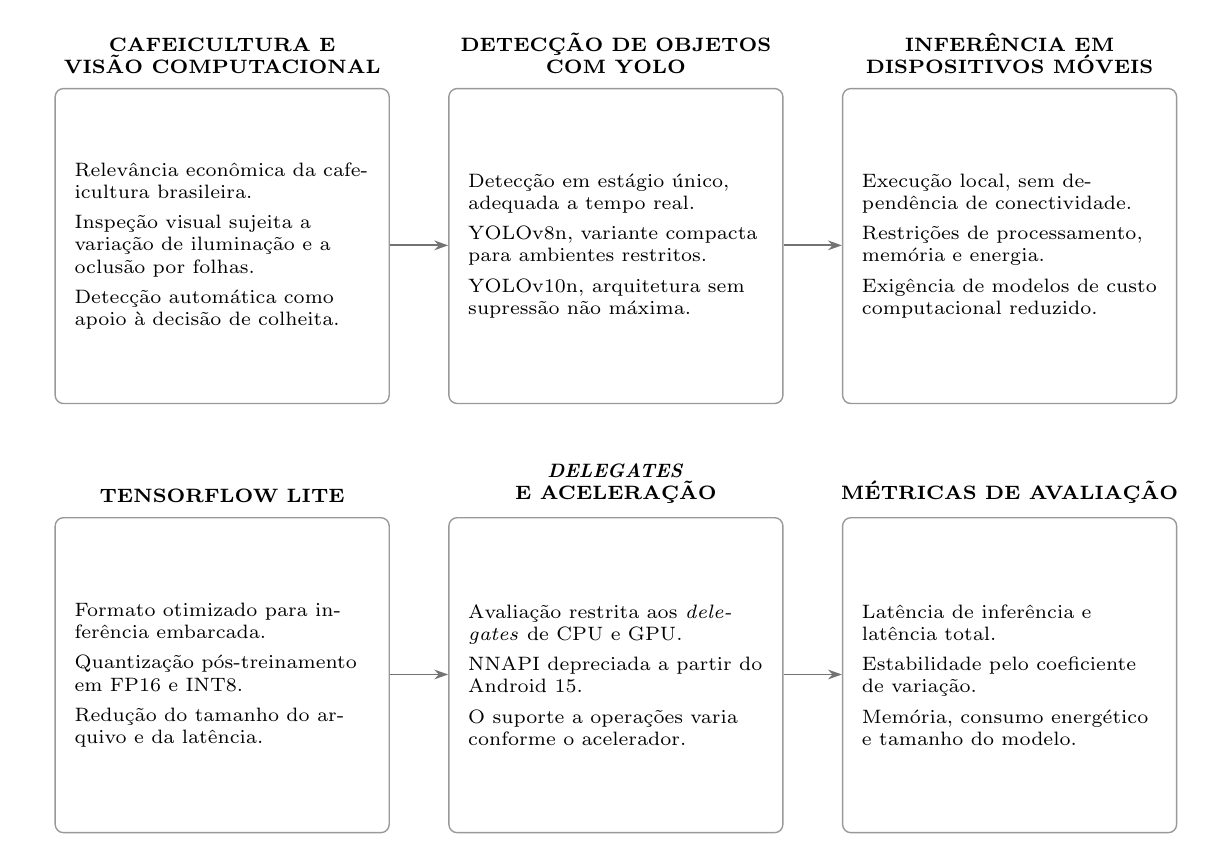
\begin{tikzpicture}[
        painel/.style={
            rectangle, rounded corners=3pt, draw=black!40, line width=0.5pt,
            text width=3.75cm, inner sep=7pt, align=left,
            minimum height=4.0cm, anchor=north, font=\scriptsize
        },
        cabeca/.style={
            font=\scriptsize\bfseries, align=center,
            text width=4.80cm, anchor=south, inner sep=2pt,
            % hifenização desligada apenas nos títulos em caixa alta
            execute at begin node={\hyphenpenalty=10000 \exhyphenpenalty=10000 }
        },
        seta/.style={-{Stealth[length=5pt,width=3.5pt]},
                     draw=black!55, line width=0.7pt}
    ]

    \def\lx{5.00}   % passo horizontal entre colunas
    \def\ly{5.45}   % passo vertical entre linhas

    % ---------------------------------------------------------- linha 1
    \node[painel] (p1) at (0,0) {%
        Relevância econômica da cafeicultura brasileira.\par\smallskip
        Inspeção visual sujeita a variação de iluminação e a oclusão por folhas.\par\smallskip
        Detecção automática como apoio à decisão de colheita.\par};
    \node[cabeca, above=3pt of p1.north] {CAFEICULTURA E\\VISÃO COMPUTACIONAL};

    \node[painel] (p2) at (\lx,0) {%
        Detecção em estágio único, adequada a tempo real.\par\smallskip
        YOLOv8n, variante compacta para ambientes restritos.\par\smallskip
        YOLOv10n, arquitetura sem supressão não máxima.\par};
    \node[cabeca, above=3pt of p2.north] {DETECÇÃO DE OBJETOS\\COM YOLO};

    \node[painel] (p3) at (2*\lx,0) {%
        Execução local, sem dependência de conectividade.\par\smallskip
        Restrições de processamento, memória e energia.\par\smallskip
        Exigência de modelos de custo computacional reduzido.\par};
    \node[cabeca, above=3pt of p3.north] {INFERÊNCIA EM\\DISPOSITIVOS MÓVEIS};

    % ---------------------------------------------------------- linha 2
    \node[painel] (p4) at (0,-\ly) {%
        Formato otimizado para inferência embarcada.\par\smallskip
        Quantização pós-treinamento em FP16 e INT8.\par\smallskip
        Redução do tamanho do arquivo e da latência.\par};
    \node[cabeca, above=3pt of p4.north] {TENSORFLOW LITE};

    \node[painel] (p5) at (\lx,-\ly) {%
        Avaliação restrita aos \textit{delegates} de CPU e GPU.\par\smallskip
        NNAPI depreciada a partir do Android~15.\par\smallskip
        O suporte a operações varia conforme o acelerador.\par};
    \node[cabeca, above=3pt of p5.north] {\textit{DELEGATES}\\E ACELERAÇÃO};

    \node[painel] (p6) at (2*\lx,-\ly) {%
        Latência de inferência e latência total.\par\smallskip
        Estabilidade pelo coeficiente de variação.\par\smallskip
        Memória, consumo energético e tamanho do modelo.\par};
    \node[cabeca, above=3pt of p6.north] {MÉTRICAS DE AVALIAÇÃO};

    % ---------------------------------------------------------- ligações
    % altura fixa, para que as setas não se inclinem caso os painéis
    % tenham alturas ligeiramente diferentes
    \draw[seta] ([yshift=-2.0cm]p1.north east) -- ([yshift=-2.0cm]p2.north west);
    \draw[seta] ([yshift=-2.0cm]p2.north east) -- ([yshift=-2.0cm]p3.north west);
    \draw[seta] ([yshift=-2.0cm]p4.north east) -- ([yshift=-2.0cm]p5.north west);
    \draw[seta] ([yshift=-2.0cm]p5.north east) -- ([yshift=-2.0cm]p6.north west);

    \end{tikzpicture}

    \legend{Elaborada pela autora (2026).}
\end{figure}


A Figura~\ref{fig:pipeline_referencial} apresenta a relação conceitual entre os principais temas discutidos neste trabalho. O fluxo inicia na aplicação de visão computacional à cafeicultura, passa pela utilização de arquiteturas \ac{YOLO} para detecção de objetos, pela inferência embarcada em dispositivos móveis e pelo uso do \ac{TFLite} como mecanismo de execução otimizada. Em seguida, são apresentados os \textit{delegates} de aceleração e as métricas utilizadas para avaliação de desempenho em \textit{smartphones} Android.

\FloatBarrier

% ─────────────────────────────────────────────────────────────────────────────
\subsection{Visão Computacional}
% ─────────────────────────────────────────────────────────────────────────────
 
Visão computacional é um campo da inteligência artificial voltado ao desenvolvimento de sistemas capazes de extrair informações de imagens e vídeos digitais. Esses sistemas são aplicados em tarefas como detecção de objetos, segmentação semântica e classificação de padrões visuais. No contexto agrícola, a visão computacional tem sido utilizada em processos de inspeção, como avaliação de maturação de frutos, identificação de pragas e estimativa de produtividade. \textcite{Eron2024Computer} apresentam uma abordagem baseada em visão computacional para monitoramento de frutos de café, utilizando YOLOv7 para detecção, classificação e estimativa de maturação em campo. Os autores discutem aplicações relacionadas à quantificação de frutos, estimativa de produtividade e monitoramento agrícola.
 
% ─────────────────────────────────────────────────────────────────────────────
\subsection{Redes Neurais Convolucionais}
% ─────────────────────────────────────────────────────────────────────────────
 
As redes neurais convolucionais (CNN, do inglês \textit{Convolutional Neural Networks})\acused{CNN} são arquiteturas de aprendizado profundo utilizadas em tarefas de visão computacional. Elas aplicam operações de convolução sobre mapas de características para extrair padrões presentes nas imagens. Camadas iniciais tendem a capturar bordas e texturas, enquanto camadas mais profundas representam padrões semânticos. Essa extração automática reduz a dependência de engenharia manual de \textit{features}. Revisões recentes indicam que essas arquiteturas são amplamente utilizadas em aplicações de classificação e detecção de padrões visuais, embora apresentem desafios relacionados a custo computacional, necessidade de dados anotados e generalização para diferentes cenários \cite{Alzubaidi2021Review}.
 
% ─────────────────────────────────────────────────────────────────────────────
\subsection{Arquitetura YOLO}
% ─────────────────────────────────────────────────────────────────────────────
 
\ac{YOLO} é uma arquitetura de detecção de objetos baseada em estágio único (\textit{single-stage detector}), proposta por \textcite{Redmon2016YOLO}. Diferentemente de métodos de dois estágios como o Faster R-CNN, o \ac{YOLO} realiza detecção e classificação em uma única passagem pela rede neural, o que reduz a latência de inferência. Ao longo de suas versões, a arquitetura incorporou mudanças relacionadas à acurácia, velocidade e detecção em múltiplas escalas. Versões compactas, como o YOLOv3-Tiny e o YOLOv8n, foram desenvolvidas para cenários com restrições computacionais. O YOLOv10 propõe detecção em tempo real de ponta a ponta, com remoção da etapa de supressão não máxima e desenho arquitetural orientado à relação entre eficiência e acurácia \cite{Wang2024YOLOv10}. \textcite{Gope2024Comparative} realizaram uma análise comparativa entre diferentes variantes da arquitetura YOLO para detecção e classificação de defeitos em grãos de café verdes. Os resultados indicaram que modelos baseados em YOLOv8n apresentaram relação entre precisão, velocidade de inferência e custo computacional compatível com aplicações de inspeção automatizada na cafeicultura.
 
% ─────────────────────────────────────────────────────────────────────────────
\subsection{TensorFlow Lite}
% ─────────────────────────────────────────────────────────────────────────────
 
O \ac{TFLite} é um \textit{framework} desenvolvido pela Google para execução de modelos de aprendizado profundo em dispositivos embarcados e móveis. Ele opera sobre modelos convertidos para o formato \texttt{.tflite}, um formato binário compacto que otimiza o grafo computacional para inferência. O processo de conversão permite aplicar técnicas como quantização pós-treinamento e fusão de operadores. O \ac{TFLite} oferece suporte a \textit{delegates} de \textit{hardware}, que permitem redirecionar partes do grafo para aceleradores dedicados disponíveis no dispositivo. \textcite{Zhao2022A} apontam o \ac{TFLite} como uma alternativa adequada para aplicações de aprendizado profundo em dispositivos móveis, especialmente em cenários com restrições de conectividade, devido à possibilidade de execução local e otimização para \textit{hardware} embarcado.
 
% ─────────────────────────────────────────────────────────────────────────────
\subsection{\textit{Delegates} do TFLite}
% ─────────────────────────────────────────────────────────────────────────────
 
Os \textit{delegates} do \ac{TFLite} são mecanismos que permitem delegar a execução de subgrafos do modelo para aceleradores de \textit{hardware} específicos do dispositivo, substituindo a execução padrão realizada pela unidade central de processamento (CPU, do inglês \textit{Central Processing Unit})\acused{CPU}. O \textit{delegate} de unidade de processamento gráfico (GPU, do inglês \textit{Graphics Processing Unit})\acused{GPU} utiliza esse recurso para paralelizar operações matriciais. A API de Redes Neurais do Android (NNAPI, do inglês \textit{Android Neural Networks API})\acused{NNAPI} direciona a inferência para aceleradores dedicados do sistema em chip (SoC, do inglês \textit{System on Chip})\acused{SoC}, como unidades de processamento neural (NPU, do inglês \textit{Neural Processing Unit})\acused{NPU} e processadores digitais de sinais (DSP, do inglês \textit{Digital Signal Processor})\acused{DSP}. O \textit{delegate} otimizado para \ac{CPU}, por sua vez, emprega instruções vetoriais do tipo instrução única e múltiplos dados (SIMD, do inglês \textit{Single Instruction, Multiple Data})\acused{SIMD} e execução multi-\textit{thread} para aproveitar os núcleos disponíveis. A escolha do \textit{delegate} afeta diretamente a latência, o consumo de energia e a estabilidade da inferência. \textcite{Chu2023nnPerf} demonstraram que o comportamento dos \textit{delegates} varia entre diferentes \acp{SoC}, indicando a necessidade de avaliação experimental em dispositivos reais. Registre-se que a \ac{NNAPI} foi depreciada a partir do Android~15, deixando de receber novos recursos e sendo desencorajada para novas aplicações; como o dispositivo utilizado neste trabalho executa Android~16, a avaliação experimental restringiu-se aos \textit{delegates} de \ac{CPU} e \ac{GPU}.
 
% ─────────────────────────────────────────────────────────────────────────────
\subsection{Quantização de Modelos}
% ─────────────────────────────────────────────────────────────────────────────
 
Quantização é uma técnica de compressão que reduz a precisão numérica dos pesos e ativações de uma rede neural. A conversão de ponto flutuante de 32~bits (FP32, do inglês \textit{Floating Point 32-bit})\acused{FP32} para inteiro de 8~bits (INT8, do inglês \textit{Integer 8-bit})\acused{INT8} diminui o tamanho do modelo em memória, o consumo de largura de banda durante a inferência e o custo energético das operações. A quantização pode ser aplicada durante o treinamento (\textit{quantization-aware training}) ou após o treinamento (\textit{post-training quantization}). A segunda abordagem é recorrente no contexto do \ac{TFLite} por não exigir retreinamento. Além do \ac{INT8}, a quantização em ponto flutuante de 16~bits (FP16, do inglês \textit{Floating Point 16-bit})\acused{FP16} representa uma alternativa que mantém maior precisão numérica, com redução de tamanho e latência em parte dos cenários. \textcite{Menghani2023Efficient} destaca que técnicas de quantização \ac{INT8} podem reduzir o custo computacional de modelos de visão computacional, diminuindo o tamanho do modelo e a latência de inferência, com variação de acurácia dependente do modelo e dos dados utilizados.
 
\subsection{Inferência em \textit{Smartphones}}

Inferência em \textit{smartphones} consiste na execução local de modelos de
aprendizado profundo diretamente no dispositivo, sem comunicação com servidores
externos. Essa abordagem, denominada \textit{on-device inference} ou
\textit{edge inference}, permite o funcionamento da aplicação sem conexão de rede
e mantém as imagens no próprio aparelho. A execução de modelos em dispositivos móveis impõe
desafios relacionados às restrições de memória de acesso aleatório (RAM, do inglês \textit{Random Access Memory})\acused{RAM}, capacidade de processamento
do \ac{SoC}, dissipação térmica e autonomia de bateria.
\textcite{Thai2024Coffee} propuseram um sistema em tempo real para
classificação de defeitos em grãos de café utilizando YOLOv8 integrado a
aplicativo móvel e infraestrutura em nuvem, demonstrando que arquiteturas
de detecção podem operar em aplicações móveis contínuas, embora com
dependência de conectividade. \textcite{Hirsch2025Exploring} investigaram a
inferência de modelos de visão computacional em \textit{smartphones} reais
heterogêneos, constatando variações de desempenho e consumo
energético entre dispositivos de diferentes gerações e faixas de preço.
 
% ─────────────────────────────────────────────────────────────────────────────
\subsection{Métricas de Desempenho para Inferência Móvel}
% ─────────────────────────────────────────────────────────────────────────────
 
A avaliação de sistemas de inferência em dispositivos móveis requer métricas além da acurácia do modelo. Entre as principais métricas utilizadas encontram-se a latência de inferência, definida como o tempo entre a entrada da imagem e a obtenção da predição; o \textit{throughput}, expresso em quadros por segundo (FPS, do inglês \textit{Frames Per Second})\acused{FPS}; o uso de \ac{RAM} durante a execução; o consumo de energia por inferência; e a estabilidade de execução, avaliada pela variabilidade da latência ao longo de inferências consecutivas. \textcite{Menghani2023Efficient} enfatiza que a escolha das métricas deve ser guiada pelo perfil da aplicação. \textcite{Hirsch2025Exploring} demonstram que modelos com latência semelhante podem apresentar consumo energético distinto dependendo do \textit{delegate} e do dispositivo utilizado.
 
% ─────────────────────────────────────────────────────────────────────────────
\subsection{Eficiência Energética em Inteligência Artificial de Borda}
% ─────────────────────────────────────────────────────────────────────────────
 
Eficiência energética é um critério central na avaliação de sistemas de inteligência artificial de borda (\textit{Edge AI}), especialmente em dispositivos alimentados por bateria. O consumo de energia durante a inferência depende da complexidade do modelo, das operações realizadas, do \textit{delegate} utilizado e das características do \ac{SoC}. Aceleradores dedicados, como \acp{NPU} e \acp{DSP}, podem apresentar menor consumo energético por operação em comparação à \ac{CPU} de propósito geral. \textcite{Zhao2022A} indicam que a combinação de quantização, poda e uso de aceleradores contribui para equilibrar desempenho e eficiência energética em aplicações de aprendizado profundo móvel.

\subsection{Anotação de Imagens e Formatos de Dados}

A construção de conjuntos de dados para detecção de objetos requer a associação entre imagens e anotações que descrevem a localização e a classe dos objetos de interesse. Em tarefas baseadas em caixas delimitadoras, cada instância anotada é representada por coordenadas espaciais e por um rótulo de classe, permitindo que o modelo aprenda simultaneamente a localizar e classificar objetos na imagem. Ferramentas de anotação, como MakeSense.ai, são utilizadas para criar essas marcações de forma visual e exportá-las em formatos compatíveis com fluxos de treinamento \cite{Makesense2024}.

Entre os formatos empregados em visão computacional está o COCO (do inglês \textit{Common Objects in Context})\acused{COCO}, frequentemente representado em Notação de Objetos JavaScript (JSON, do inglês \textit{JavaScript Object Notation})\acused{JSON}, e o formato utilizado em modelos \ac{YOLO}. O formato \ac{COCO} organiza imagens, categorias e anotações em uma estrutura única, enquanto o formato \ac{YOLO} representa cada anotação em arquivos de texto associados às imagens, com coordenadas normalizadas das caixas delimitadoras. A escolha do formato afeta a compatibilidade com bibliotecas de treinamento, ferramentas de validação e rotinas de conversão dos dados.

\subsection{Curadoria, Redundância Visual e \textit{Perceptual Hashing}}

Em conjuntos de imagens coletadas em campo, é comum que fotografias sucessivas apresentem ângulos, enquadramentos e conteúdo visual semelhantes. Essa redundância pode reduzir a diversidade efetiva do conjunto de treinamento e favorecer vieses durante o ajuste do modelo. Uma estratégia para identificar imagens visualmente semelhantes é o \textit{Perceptual Hashing} (pHash), que gera uma assinatura compacta da imagem e permite comparar pares de amostras por meio de medidas de distância entre os respectivos hashes.

O pHash pode ser implementado a partir da \ac{DCT}, utilizando componentes de baixa frequência para representar características globais da imagem. Diferenças pequenas entre hashes indicam maior similaridade visual, o que permite selecionar amostras redundantes para revisão ou remoção. \textcite{Zauner2010ImplementationAB} discute a implementação e avaliação de funções de hash perceptual, fundamentando o uso desse tipo de técnica na etapa de curadoria dos dados.

\subsection{Transferência de Aprendizado, Aumento de Dados e Treinamento}

O treinamento de modelos de detecção em bases específicas pode se beneficiar da transferência de aprendizado, na qual pesos previamente ajustados em bases amplas são utilizados como ponto de partida para uma nova tarefa. Essa estratégia reduz a necessidade de iniciar o treinamento do zero e pode melhorar a convergência quando o conjunto de dados do problema-alvo é limitado. No contexto de visão computacional, pesos pré-treinados em bases como \ac{COCO} são frequentemente empregados antes do ajuste fino (\textit{fine-tuning}) em dados específicos \cite{Tan2023TransferLearning}.

O aumento artificial de dados (\textit{data augmentation}) é outra estratégia usada para ampliar a variabilidade das amostras apresentadas ao modelo. Transformações como espelhamento, variações de brilho, rotação, translação, alteração de escala e composição por mosaico permitem simular condições visuais distintas sem coletar novas imagens. Revisões sobre aumento de dados indicam que essas técnicas podem reduzir sobreajuste e melhorar a capacidade de generalização de modelos de aprendizado profundo, desde que sejam compatíveis com o domínio da aplicação \cite{Shorten2019,Mumuni2022DataAugmentation}. Em arquiteturas da família \ac{YOLO}, estratégias como o mosaico também foram utilizadas para aumentar a diversidade espacial das amostras durante o treinamento \cite{Bochkovskiy2020YOLOv4}.

\subsection{Aplicações Android e Coleta de Métricas no Dispositivo}

Aplicações Android voltadas à inferência local integram a interface de captura ou seleção de imagens, o pré-processamento, a execução do modelo e a apresentação dos resultados ao usuário. O uso de \textit{frameworks} como Flutter permite desenvolver interfaces móveis e integrar recursos do dispositivo, facilitando a criação de protótipos experimentais para avaliação de modelos em ambiente real de uso \cite{Flutter2024}.

Além de exibir as detecções, a aplicação pode atuar como instrumento de coleta de métricas computacionais. Indicadores como tempo de inferência, taxa de quadros por segundo, consumo de memória, temperatura e consumo energético permitem avaliar a viabilidade prática do modelo no dispositivo. Em sistemas Android, essas medições podem ser obtidas por registros internos da aplicação e por recursos do sistema operacional, como APIs de bateria e ferramentas de monitoramento. Esse tipo de avaliação demonstra que os resultados obtidos em ambiente de desenvolvimento nem sempre refletem o comportamento observado em \textit{smartphones} reais, nos quais há variação de \textit{hardware}, gerenciamento térmico e concorrência por recursos \cite{Chu2023nnPerf,Hirsch2025Exploring}.
 
% ─────────────────────────────────────────────────────────────────────────────
\subsection{Análise Bibliométrica}
% ─────────────────────────────────────────────────────────────────────────────

Foi realizada uma análise bibliométrica a partir de buscas conduzidas na base de dados Scopus, utilizando consultas relacionadas a arquiteturas \ac{YOLO}, inferência móvel, \textit{Edge AI}, \ac{TFLite}, quantização e aplicações de visão computacional na cafeicultura. Os dados foram analisados com auxílio da linguagem Python e das bibliotecas Pandas, Matplotlib e NetworkX, permitindo a construção de visualizações relacionadas à evolução temporal das publicações, concentração temática, frequência de termos nos títulos e relações conceituais entre os tópicos investigados.

A Figura~\ref{fig:crescimento_temporal} apresenta a evolução anual do número de registros entre 2021 e 2025. As publicações que associam \ac{YOLO} à execução em dispositivos móveis passam de 38 em 2021 para 736 em 2025 e multiplicam-se por mais de cinco apenas entre 2023 e 2025. Os registros envolvendo \ac{TFLite} mantêm-se entre 42 e 65 até 2024 e somente em 2025 alcançam 154. A aplicação de \ac{YOLO} na cafeicultura permanece em volume reduzido ao longo de todo o período, de 3 registros em 2021 a 30 em 2025, com expansão perceptível a partir de 2024. O ano de 2026, ainda em curso no momento da consulta, foi excluído da série por não ser comparável aos demais.

\begin{figure}[H]
    \centering
    \caption{Evolução anual do número de registros recuperados por tópico de busca, de 2021 a 2025}
    \figuraHorizontal{figuras/crescimento_temporal.pdf}
    \legend{Elaborada pela autora (2026), com base em dados extraídos da base Scopus.}
    \label{fig:crescimento_temporal}
\end{figure}

A Figura~\ref{fig:topicos} apresenta o número de registros recuperados por tópico de busca. O maior volume corresponde à quantização de modelos, com 1.400 registros, seguida de perto pelas arquiteturas \ac{YOLO} aplicadas a dispositivos móveis, com 1.256; a proximidade entre os dois indica que a otimização numérica acompanha o interesse pelos detectores, e não o sucede. Em patamar inferior situam-se a visão computacional aplicada à agricultura, com 448 registros, e o \ac{TFLite}, com 370. A interseção entre cafeicultura e \ac{YOLO} responde pelo menor volume de todos, 73 registros, cerca de dezenove vezes menor que o do tópico mais frequente, o que evidencia tratar-se de um nicho ainda específico dentro da literatura recente.

\begin{figure}[H]
    \centering
    \caption{Número de registros recuperados por tópico de busca}
    \figuraHorizontal{figuras/topicos_busca.pdf}
    \legend{Elaborada pela autora (2026), com base em dados extraídos da base Scopus.}
    \label{fig:topicos}
\end{figure}

A Figura~\ref{fig:keywords} apresenta os quinze termos mais frequentes nos títulos dos 3.401 registros distintos recuperados pelas cinco consultas, contados pelo número de títulos em que cada termo ocorre. As primeiras posições reproduzem a própria expressão de busca, caso de \textit{detection}, \textit{network}, \textit{deep}, \textit{learning} e \textit{neural}, e por isso pouco informam sobre o conteúdo. Abaixo delas, \textit{lightweight}, em 422 títulos, e \textit{real-time}, em 376, revelam a procura por modelos de menor custo computacional e por execução em tempo real, enquanto \textit{edge}, \textit{mobile} e \textit{embedded}, entre 247 e 268 títulos, situam a tarefa no contexto de execução local em dispositivos com restrição de recursos. Os termos ligados à aplicação agrícola ocupam faixa inferior à das quinze posições exibidas, com \textit{fruit} em 215 títulos, \textit{disease} em 147 e \textit{defect} em 127, ao passo que \textit{ripeness} e \textit{maturity} ocorrem em 88 e em 81. A predominância da detecção de defeitos e de doenças sobre a avaliação do estágio de maturação delimita a lacuna de que trata este trabalho.

\begin{figure}[H]
    \centering
    \caption{Quinze termos mais frequentes nos títulos dos trabalhos recuperados}
    \figuraHorizontal{figuras/termos_titulos.pdf}
    \legend{Elaborada pela autora (2026), com base em dados extraídos da base Scopus.}
    \label{fig:keywords}
\end{figure}

A Figura~\ref{fig:rede_tematica} organiza em forma de rede os conceitos recorrentes no \textit{corpus} bibliográfico e as ligações observadas entre eles. O núcleo é formado pela arquitetura \ac{YOLO} e pelos termos diretamente associados à detecção em tempo real, do qual parte um ramo voltado à execução embarcada que reúne \ac{TFLite}, \ac{GPU}, \ac{NNAPI}, Android e inferência móvel. Os conceitos ligados à cafeicultura e à visão computacional agrícola conectam-se ao núcleo por um único caminho e não se articulam com esse ramo, o que sugere que ainda são poucos os trabalhos a avaliar experimentalmente diferentes \textit{delegates} em cenários agrícolas reais.

% =====================================================================
% Figura 5 — Rede temática do corpus bibliográfico.
%
% Substitui grafico_4_rede_tematica_sem_margem.png. A versão anterior
% deixava um quadrante inteiro vazio e distribuía os nós sem relação com
% a distância conceitual que o texto descreve. Aqui o núcleo técnico
% ocupa o centro, o ramo de execução embarcada desce à direita e o ramo
% agrícola, descrito no texto como periférico, fica à esquerda.
%
% REQUER no preâmbulo (já presentes em artigo.tex):
%   \usepackage{tikz}
%   \usetikzlibrary{positioning, arrows.meta}
% =====================================================================

\begin{figure}[H]
    \centering
    \caption{Rede temática dos conceitos recorrentes no \textit{corpus} bibliográfico}
    \label{fig:rede_tematica}

    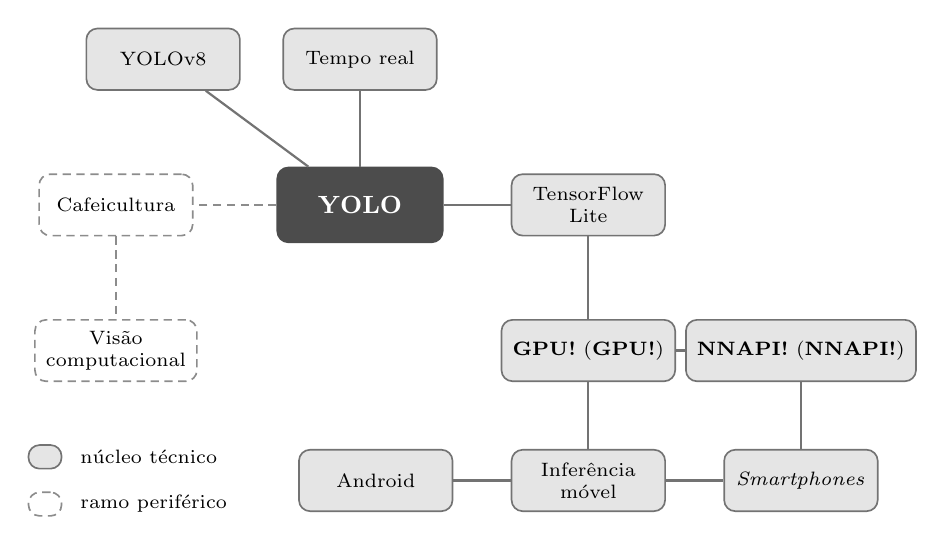
\begin{tikzpicture}[
        every node/.style={font=\scriptsize},
        no/.style={
            rectangle, rounded corners=4pt, draw, line width=0.6pt,
            align=center, inner sep=4pt, minimum height=0.78cm,
            minimum width=1.95cm
        },
        nucleo/.style={no, draw=black!70, fill=black!70, text=white,
                       font=\small\bfseries, minimum width=2.1cm,
                       minimum height=0.95cm},
        tecnico/.style={no, draw=black!55, fill=black!10},
        periferico/.style={no, draw=black!45, fill=white,
                           densely dashed},
        lig/.style={draw=black!55, line width=0.8pt},
        ligp/.style={draw=black!45, line width=0.8pt, densely dashed}
    ]

    % ------------------------------------------------- núcleo
    \node[nucleo] (yolo) at (0,0) {YOLO};

    % ------------------------------------------------- ramo de detecção
    \node[tecnico] (v8)    at (-2.5, 1.85) {YOLOv8};
    \node[tecnico] (tempo) at ( 0.0, 1.85) {Tempo real};
    \node[tecnico] (tfl)   at ( 2.9, 0.00) {TensorFlow\\Lite};

    % --------------------------------------- ramo de execução embarcada
    \node[tecnico] (gpu)   at ( 2.9,-1.85) {\ac{GPU}};
    \node[tecnico] (nnapi) at ( 5.6,-1.85) {\ac{NNAPI}};
    \node[tecnico] (infm)  at ( 2.9,-3.50) {Inferência\\móvel};
    \node[tecnico] (andr)  at ( 0.2,-3.50) {Android};
    \node[tecnico] (smart) at ( 5.6,-3.50) {\textit{Smartphones}};

    % ------------------------------------------------- ramo agrícola
    \node[periferico] (cafe) at (-3.1, 0.00) {Cafeicultura};
    \node[periferico] (visao) at (-3.1,-1.85) {Visão\\computacional};

    % ------------------------------------------------- arestas
    \draw[lig] (yolo) -- (v8);
    \draw[lig] (yolo) -- (tempo);
    \draw[lig] (yolo) -- (tfl);
    \draw[lig] (tfl)  -- (gpu);
    \draw[lig] (gpu)  -- (nnapi);
    \draw[lig] (gpu)  -- (infm);
    \draw[lig] (infm) -- (andr);
    \draw[lig] (infm) -- (smart);
    \draw[lig] (nnapi) -- (smart);
    \draw[ligp] (yolo) -- (cafe);
    \draw[ligp] (cafe) -- (visao);

    % ------------------------------------------------- legenda interna
    \node[tecnico, minimum width=0.42cm, minimum height=0.30cm,
          inner sep=0pt] (lg1) at (-4.0,-3.20) {};
    \node[anchor=west, font=\scriptsize] at ([xshift=3pt]lg1.east)
        {núcleo técnico};
    \node[periferico, minimum width=0.42cm, minimum height=0.30cm,
          inner sep=0pt] (lg2) at (-4.0,-3.80) {};
    \node[anchor=west, font=\scriptsize] at ([xshift=3pt]lg2.east)
        {ramo periférico};

    \end{tikzpicture}

    \legend{Elaborada pela autora (2026).}
\end{figure}


A análise bibliométrica evidencia crescimento recente das pesquisas relacionadas a arquiteturas \ac{YOLO}, inferência móvel e aplicações de \textit{Edge AI}, com atenção crescente ao uso do \ac{TFLite}, à aceleração por \ac{GPU} e à execução em dispositivos Android. As aplicações agrícolas recuperadas, por sua vez, concentram-se na detecção de defeitos e de doenças. Trabalhos que integrem simultaneamente inferência móvel, avaliação de \textit{delegates} e cafeicultura permanecem limitados, o que caracteriza a lacuna explorada pelo presente trabalho.
 
% ─────────────────────────────────────────────────────────────────────────────
\subsection{Trabalhos Relacionados}
% ─────────────────────────────────────────────────────────────────────────────

Os trabalhos relacionados foram analisados considerando três eixos principais, correspondentes a aplicações de visão computacional na cafeicultura, variantes da arquitetura \ac{YOLO} e estratégias de inferência em dispositivos móveis. Essa organização permite comparar métodos, bases utilizadas, métricas reportadas e limitações associadas à execução em ambientes reais.

Em 2021, \textcite{Bazame2021Detection}, a detecção da maturação de frutos de café
foi tratada como uma tarefa de detecção, classificação e mapeamento durante a
colheita. Os autores utilizaram YOLOv3-Tiny com pesos pré-treinados, aumento de
dados, anotações por caixas delimitadoras e três classes de maturação,
correspondentes a frutos verdes, cereja e passa. O conjunto experimental foi composto por 400 imagens
extraídas de vídeos de colheita, sendo 280 destinadas ao treinamento e 120 à
validação. O melhor resultado foi obtido com entrada de 800~$\times$~800~pixels,
alcançando 84,0\% de média da precisão média (mAP, do inglês \textit{mean Average Precision})\acused{mAP}, 83,0\% de precisão, 82,0\% de revocação (\textit{recall}) e 82,0\% de
F1-score. Por classe, as precisões médias foram de aproximadamente 86,0\% para
frutos verdes, 85,0\% para frutos cereja e 80,0\% para frutos passa, indicando
maior dificuldade na separação entre frutos maduros e sobremaduros.

Ainda em 2021, a revisão de \textcite{Alzubaidi2021Review} descreve conceitos, arquiteturas e aplicações de aprendizado profundo, com destaque para o papel das \ac{CNN} em tarefas de visão computacional. O estudo também aponta desafios recorrentes, como demanda por bases de dados representativas, custo computacional, escolha de arquitetura e capacidade de generalização. A detecção de frutos de café em campo envolve variações de iluminação, oclusão e aparência dos objetos, exigindo modelos capazes de extrair características visuais robustas.

Em 2022, \textcite{Zhao2022A} discutem a inferência móvel a partir de
aplicações, oportunidades e desafios de implantação de aprendizado profundo em
dispositivos com restrição de processamento, memória e energia. Os autores
analisam estratégias como compressão de modelos, quantização, aceleração por
\textit{hardware}, execução local e uso de \textit{frameworks} voltados a
plataformas móveis, incluindo o \ac{TFLite}. Embora o trabalho também seja uma
revisão e não reporte uma precisão única, ele evidencia que a avaliação de
modelos móveis deve considerar não apenas acurácia, mas também latência,
consumo energético, compatibilidade com dispositivos e estabilidade de execução.

Em 2023, no estudo de \textcite{Chu2023nnPerf}, a contribuição principal não se concentra na proposição de uma
nova arquitetura de detecção, mas no desenvolvimento de uma ferramenta de \textit{profiling} para
analisar a latência de inferência de redes neurais em plataformas móveis. O
nnPerf foi proposto para medir o tempo de execução em nível de
operadores e \textit{kernels}, permitindo observar gargalos que não aparecem
quando se considera apenas a latência total do modelo. Os autores discutem que o
comportamento da inferência varia conforme o \ac{SoC}, o \textit{delegate} e as
operações usadas pela rede, aspecto que reforça a necessidade de avaliar
modelos em dispositivos reais, e não apenas em ambiente de desenvolvimento.

Em 2023, \textcite{Menghani2023Efficient} discutem técnicas de eficiência
para modelos de aprendizado profundo, como quantização, poda, fatoração de
matrizes, arquiteturas compactas e destilação de conhecimento. Por se tratar de
uma revisão, o estudo não apresenta uma única taxa de precisão ou um único
experimento agrícola, mas organiza evidências de que a redução de tamanho e
latência dos modelos deve ser analisada juntamente com possíveis perdas de
acurácia. A escolha entre representações de oito ou dezesseis bits pode alterar simultaneamente tamanho do arquivo, tempo de inferência e desempenho preditivo.

No contexto específico da cafeicultura, \textcite{Eron2024Computer} apresentam
uma abordagem de monitoramento inteligente baseada em visão computacional para
quantificação, classificação e estimativa de maturação de frutos de café. O
trabalho utiliza imagens coletadas em campo e modelo baseado em YOLOv7 para
identificar frutos e apoiar análises relacionadas à produção sustentável. A
contribuição do estudo está na aplicação de detecção de objetos ao monitoramento
da cultura do café, embora não aprofunde a avaliação de execução local em
\textit{smartphones} Android ou o impacto de estratégias de quantização.

Para \textcite{Gope2024Comparative}, a comparação entre variantes do \ac{YOLO} foi
aplicada à detecção e classificação de defeitos em grãos verdes de café. O
estudo utilizou 4.032 imagens de treinamento e 506 imagens de teste, com
resolução padronizada em 640~$\times$~640~pixels, comparando YOLOv3, YOLOv4,
YOLOv5, YOLOv7, YOLOv8 e versões customizadas. Entre os modelos avaliados, o
custom-YOLOv8n apresentou os melhores resultados, com 0,977 de precisão, 0,990
de revocação, 0,983 de F1-score e 0,995 de mAP. Esses valores indicam desempenho elevado para inspeção de defeitos em grãos; contudo, o estudo foi conduzido fora
do cenário de inferência móvel em dispositivos Android.

Enquanto \textcite{Kazama2024Monitoring} investigaram diretamente a maturação de
frutos de café antes da colheita, o foco esteve na robustez do modelo frente a
diferentes condições de aquisição de imagem. Os autores modificaram o YOLOv8n
com o módulo RFCAConv e avaliaram imagens obtidas sob iluminação natural e
artificial, em diferentes enquadramentos da planta e dos ramos. O modelo
proposto alcançou mAP@0,50 de 74,20\%, superando o YOLOv8n padrão em 1,90 ponto
percentual, com mAP@0,95 de 45,90\%. As precisões médias por classe foram de
73,40\% para frutos verdes, 67,10\% para semimaduros, 74,40\% para maduros e
71,90\% para sobremaduros. Os resultados evidenciam a dificuldade da classificação em
campo, especialmente pela proximidade visual entre estágios de maturação.

Na mesma direção, \textcite{Ye2025ASD} propuseram o ASD-YOLO, construído
sobre o YOLOv7 com a introdução de atenção L-Norm, do módulo SPD-Conv e do
redimensionador DySample, voltado à detecção da maturação de frutos de café
em cenários com oclusão entre folhas e frutos. O trabalho reporta revocação
de 78,4\%, precisão de 69,8\% e \ac{mAP} de 80,1\%, com ganho de 2,1
pontos percentuais sobre o YOLOv7. A avaliação foi conduzida em ambiente de
desenvolvimento, sem medição de execução em \textit{smartphones}, de modo
que o custo da arquitetura proposta em processadores móveis permanece não
verificado.

Já no trabalho de \textcite{Wang2024YOLOv10}, a contribuição está associada à proposição
do YOLOv10 como uma arquitetura de detecção em tempo real de ponta a ponta, com
remoção da etapa de supressão não máxima no pós-processamento. Na avaliação em
COCO, a versão YOLOv10-N apresentou 2,3 milhões de parâmetros, 6,7 bilhões de
operações e precisão média (AP, do inglês \textit{Average Precision}) de 38,5\%, com latência reportada de 1,84~ms; versões maiores,
como YOLOv10-X, chegaram a AP de 54,4\%, com 29,5 milhões de parâmetros e
latência de 10,70~ms. Esses resultados indicam a relação entre escala do modelo,
acurácia e latência, mas não contemplam cafeicultura nem execução em
\textit{smartphones} Android com \ac{TFLite}.

No trabalho de \textcite{Thai2024Coffee}, a classificação automática de defeitos
em grãos de café foi tratada por meio de um sistema em tempo real baseado em
YOLOv8, OpenCV (\textit{Open Source Computer Vision Library})\acused{OpenCV}, aplicativo móvel e infraestrutura em nuvem. O sistema foi
proposto para classificar nove variedades ou categorias associadas à qualidade
dos grãos, com tempo de resposta reportado entre 1 e 3 segundos. Embora a
integração com aplicação móvel relacione o estudo a um cenário aplicado, a
solução depende de infraestrutura em nuvem, diferentemente da execução
local no dispositivo considerada no presente trabalho.

Por fim, em \textcite{Hirsch2025Exploring}, a inferência de modelos de visão
computacional foi avaliada em \textit{smartphones} reais heterogêneos, com foco
em latência acumulada, consumo de energia e viabilidade de execução em
ambientes de borda. O estudo utiliza ambientes de teste reais e discute como
diferenças entre dispositivos, carga de trabalho e organização da execução podem
afetar o desempenho observado. Apesar de não se concentrar em modelos \ac{YOLO}
nem em imagens agrícolas, o trabalho é relevante por indicar que métricas como
energia, estabilidade e latência em dispositivos reais são necessárias à
avaliação da viabilidade prática de aplicações móveis de visão computacional. O Quadro~\ref{quad:survey} sintetiza os trabalhos apresentados em ordem
cronológica, destacando a abordagem utilizada, os principais resultados,
as limitações observadas e a relação de cada estudo com a proposta deste
trabalho.

\FloatBarrier

\begin{board}[H]
\centering
\caption{Síntese dos trabalhos relacionados}
\label{quad:survey}
\scriptsize
\setlength{\tabcolsep}{2pt}
\renewcommand{\arraystretch}{1.02}
\makebox[\textwidth][c]{%
\resizebox{0.94\textwidth}{!}{%
\begin{tabular}{c p{3.0cm} p{3.6cm} p{4.0cm} p{4.3cm}}
\toprule
\textbf{Ano} & \textbf{Autores} & \textbf{Abordagem} & \textbf{Resultados e limitações} &
\textbf{Relação com este trabalho} \\
\midrule
2021 & \textcite{Bazame2021Detection} & YOLOv3-Tiny para detectar, classificar e mapear
frutos de café em 400 imagens de campo. & Obteve mAP de 84,0\%, precisão de
83,0\%, revocação de 82,0\% e F1-score de 82,0\%; não avaliou inferência móvel,
energia ou estabilidade. & Mostra a viabilidade de modelos \ac{YOLO} para
classes de maturação em lavouras de café. \\
\midrule
2021 & \textcite{Alzubaidi2021Review} & Revisão sobre aprendizado profundo, arquiteturas de \ac{CNN}, desafios e aplicações. & Discute conceitos fundamentais, aplicações e limitações de modelos profundos, incluindo custo computacional e generalização. & Fundamenta o uso de \ac{CNN} e modelos de visão computacional no referencial teórico. \\
\midrule
2022 & \textcite{Zhao2022A} & Revisão sobre inferência de aprendizado profundo
em dispositivos móveis. & Analisa acurácia, latência, energia, memória e
compatibilidade; não foca em \ac{YOLO} aplicado à cafeicultura. & Apoia a
discussão sobre implantação de modelos em \textit{smartphones}. \\
\midrule
2023 & \textcite{Chu2023nnPerf} & nnPerf para \textit{profiling} de
inferência com \ac{TFLite} em plataformas móveis. & Mede latência por operador,
\textit{kernel} e \ac{SoC}; não aborda cafeicultura nem maturação de frutos. &
Evidencia variação de desempenho entre \textit{delegates} e dispositivos. \\
\midrule
2023 & \textcite{Menghani2023Efficient} & Revisão sobre quantização, poda, compressão e
destilação em aprendizado profundo. & Discute redução de tamanho, latência e
custo computacional; não apresenta experimento agrícola ou em dispositivos
reais. & Fundamenta a escolha de quantização e métricas de eficiência. \\
\midrule
2024 & \textcite{Eron2024Computer} & Monitoramento inteligente do café com visão computacional e modelo baseado em YOLOv7. & Avalia detecção, quantificação e estimativa de maturação em imagens de campo; não avalia execução em \textit{smartphones}. & Contextualiza o uso de visão computacional no café. \\
\midrule
2024 & \textcite{Gope2024Comparative} & Comparação entre YOLOv3, YOLOv4, YOLOv5, YOLOv7,
YOLOv8 e custom-YOLOv8n para defeitos em grãos verdes. & Obteve precisão de
0,977, revocação de 0,990, F1-score de 0,983 e mAP de 0,995; não avaliou
inferência móvel. & Indica potencial de variantes compactas de \ac{YOLO} para
inspeção do café. \\
\midrule
2024 & \textcite{Kazama2024Monitoring} & YOLOv8n com RFCAConv para classificação de
estágios de maturação de frutos de café em campo. & Obteve mAP@0,50 de 74,20\%
e mAP@0,95 de 45,90\%; não avaliou \textit{smartphones} nem consumo energético.
& Reforça a maturação de frutos como tarefa relevante de detecção. \\
\midrule
2024 & \textcite{Wang2024YOLOv10} & YOLOv10 para detecção em tempo real de
ponta a ponta, sem supressão não máxima. & YOLOv10-N obteve AP de 38,5\% e latência de
1,84~ms; não aborda cafeicultura ou \ac{TFLite} Android. & Justifica a inclusão
do YOLOv10 na comparação experimental. \\
\midrule
2024 & \textcite{Thai2024Coffee} & YOLOv8, OpenCV, aplicativo móvel e nuvem para
classificação de defeitos em grãos de café. & Tempo de resposta entre 1 e 3
segundos; depende de conectividade e processamento em nuvem. & Motiva a
execução local para reduzir dependência de rede. \\
\midrule
2025 & \textcite{Ye2025ASD} & ASD-YOLO, sobre o YOLOv7, com atenção
L-Norm, SPD-Conv e DySample, para detecção da maturação de frutos de café sob
oclusão. & Obteve \ac{mAP} de 80,1\%, precisão de 69,8\% e revocação de
78,4\%; não avaliou execução em \textit{smartphones}. & Indica que a
classificação de maturação parte de detectores ajustados a esse fim. \\
\midrule
2025 & \textcite{Hirsch2025Exploring} & Avaliação de inferência de visão computacional em
\textit{smartphones} reais heterogêneos. & Mede latência, energia e viabilidade
de execução; não foca em \ac{YOLO} ou cafeicultura. & Fundamenta avaliação em
dispositivos reais e métricas de estabilidade. \\
\midrule
2026 & \textbf{Este trabalho} & \textbf{YOLOv8n e YOLOv10n convertidos para
\ac{TFLite}, aplicados a um conjunto próprio de 2.168 imagens
coletadas em Bambuí.} & \textbf{Alcançou \ac{mAP}@0,50 de 0,6455 e 0,6419 no
conjunto de teste; \ac{GPU} acelera o YOLOv8n em 4,7$\times$ e não
acelera o YOLOv10n, cuja variante \ac{INT8} não é executável nesse
\textit{delegate}.} &
\textbf{Compara quantização \ac{INT8}/\ac{FP16} e \textit{delegates}
\ac{CPU}/\ac{GPU} em dispositivos Android reais.} \\
\bottomrule
\end{tabular}%
}%
}
\legend{Elaborada pela autora (2026).}
\end{board}

\FloatBarrier

A análise dos trabalhos relacionados indica avanços na
aplicação de modelos \ac{YOLO} à cafeicultura e na execução de redes neurais
em dispositivos móveis. No entanto, ainda são limitados os estudos que combinam
esses dois eixos com foco em comparação de \textit{delegates}
do \ac{TFLite} em \textit{smartphones} reais aplicados à detecção de maturação
de frutos de café.

O presente trabalho se distingue dos estudos anteriores por quatro aspectos. O
primeiro é o uso de um conjunto de dados próprio, composto por aproximadamente
5.000 imagens coletadas em lavouras de campo aberto na região de Bambuí, Minas Gerais, entre novembro de 2023 e fevereiro de 2024, período correspondente ao ciclo de maturação dos frutos de café na região. Os
trabalhos analisados não reportam dados coletados nessa região ou com esse
contexto de produção. O segundo é a orientação prática da classificação, cujo
objetivo é fornecer ao produtor rural uma indicação sobre o momento adequado
para a colheita, com base em estágios de maturação a serem definidos a partir de
critérios agronômicos específicos para a região. O terceiro é a avaliação de
duas estratégias de quantização pós-treinamento, \ac{INT8} e \ac{FP16},
a serem aplicadas aos modelos YOLOv8n e YOLOv10n, permitindo comparar o impacto de cada abordagem
sobre acurácia, tamanho do modelo e latência de inferência. O quarto é a
comparação sistemática dos \textit{delegates} de \ac{CPU} e \ac{GPU} do
\ac{TFLite} em \textit{smartphones} Android reais de diferentes gerações e
faixas de preço, medindo latência, estabilidade de execução e consumo
energético. Enquanto \textcite{Hirsch2025Exploring} avaliam inferência móvel
sem uso de \ac{YOLO} e \textcite{Chu2023nnPerf} investigam
\textit{profiling} sem aplicação à cafeicultura, o presente trabalho integra
essas duas dimensões em um único experimento aplicado ao contexto real da
cafeicultura brasileira.

\FloatBarrier

\section{METODOLOGIA}
\label{sec:metodologia}

Esta pesquisa caracteriza-se como aplicada, de abordagem quantitativa e natureza experimental, tendo como objetivo avaliar o desempenho de modelos de detecção de objetos executados localmente em dispositivos móveis Android. O procedimento metodológico foi estruturado com base na literatura sobre visão computacional aplicada à cafeicultura, inferência embarcada e otimização de modelos para dispositivos com recursos computacionais limitados, permitindo definir as etapas experimentais adotadas ao longo do desenvolvimento da pesquisa.

De forma geral, o estudo compreende a construção e organização do conjunto de dados, o treinamento de modelos da família YOLO, a conversão para o formato TensorFlow Lite, a integração em uma aplicação Android e a avaliação experimental considerando diferentes estratégias de quantização e mecanismos de aceleração por \textit{hardware}. As análises contemplam tanto métricas relacionadas à qualidade da detecção quanto indicadores associados ao desempenho computacional durante a inferência em \textit{smartphones}. A Figura~\ref{fig:fluxo_metodologia} apresenta uma visão geral das etapas que compõem o procedimento metodológico adotado nesta pesquisa, desde a aquisição das imagens até a comparação das configurações experimentais avaliadas.

\begin{figure}[H]
\centering
\caption{Fluxo metodológico do trabalho}
\label{fig:fluxo_metodologia}

\makebox[\textwidth][c]{%
\begin{adjustbox}{max width=\textwidth,max totalheight=0.88\textheight,center}
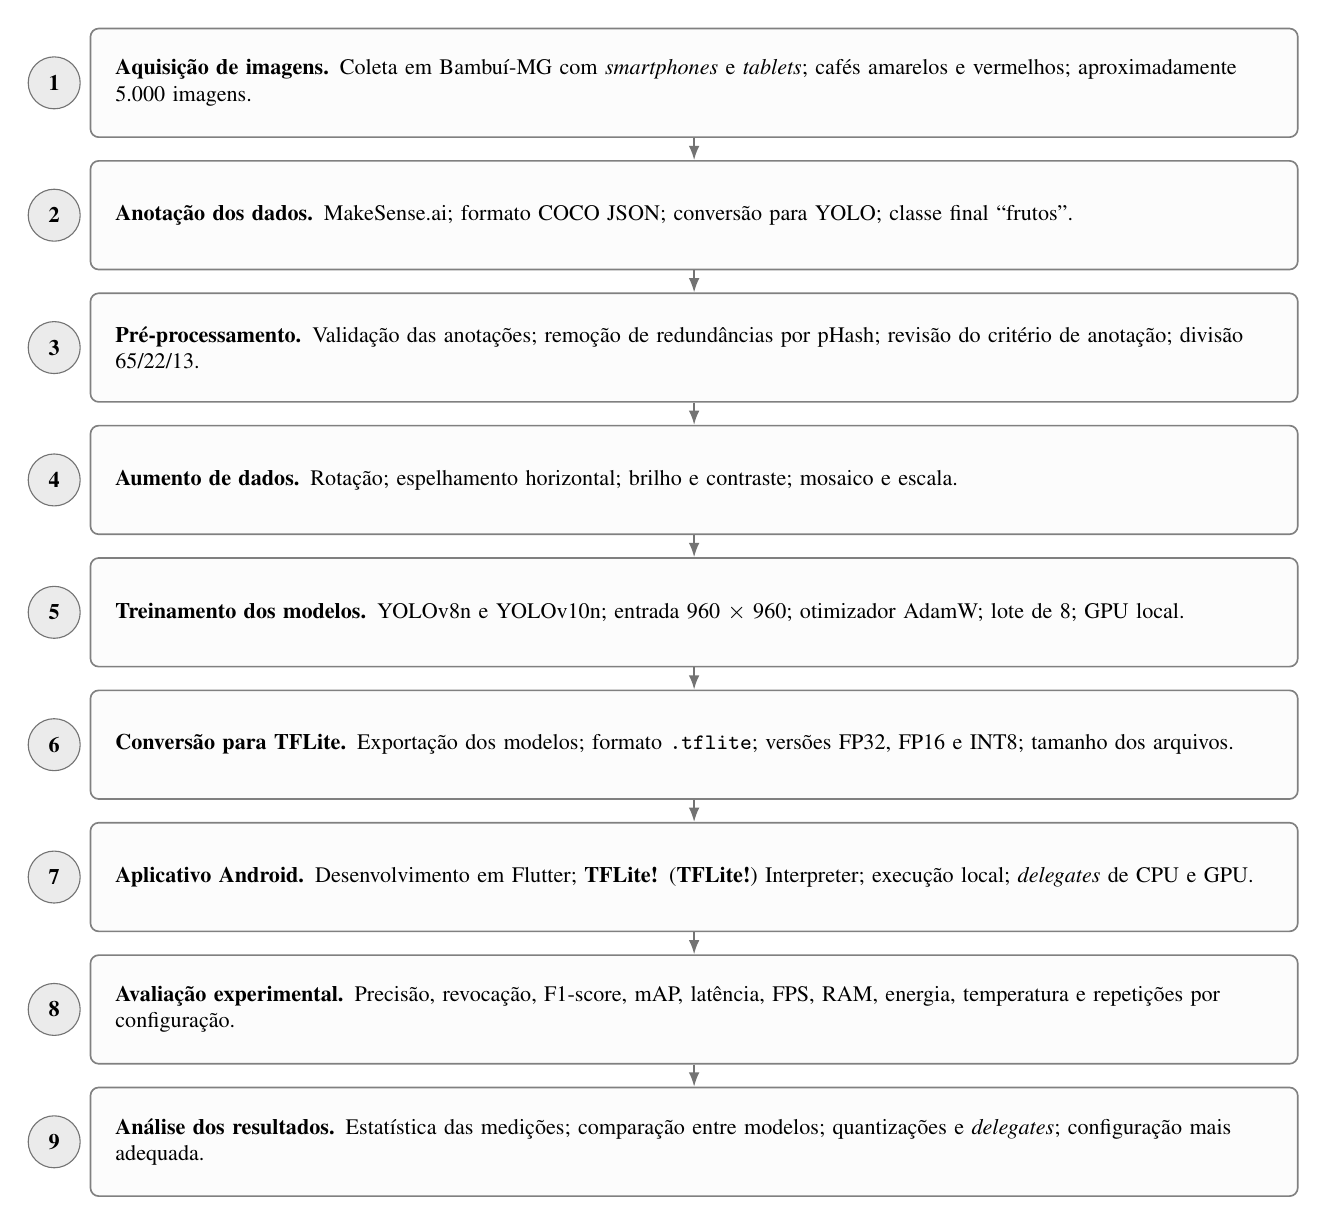
\begin{tikzpicture}[
    font=\fontfamily{ptm}\selectfont\footnotesize,
    etapa/.style={
        rectangle,
        rounded corners=3pt,
        draw=black!50,
        fill=black!1,
        line width=0.6pt,
        text width=14.7cm,
        minimum height=1.38cm,
        align=left,
        inner xsep=9pt,
        inner ysep=7pt
    },
    numero/.style={
        circle,
        draw=black!55,
        fill=black!8,
        minimum size=6.6mm,
        inner sep=0pt,
        font=\fontfamily{ptm}\selectfont\bfseries\footnotesize
    },
    seta/.style={-{Latex[length=1.8mm]}, line width=0.6pt, draw=black!55}
]

\node[etapa] (e1) at (0,0) {\textbf{Aquisição de imagens.} Coleta em Bambuí-MG com \textit{smartphones} e \textit{tablets}; cafés amarelos e vermelhos; aproximadamente 5.000 imagens.};
\node[numero] at ([xshift=-4.5mm]e1.west) {1};

\node[etapa, below=0.28cm of e1] (e2) {\textbf{Anotação dos dados.} MakeSense.ai; formato COCO JSON; conversão para YOLO; classe final ``frutos''.};
\node[numero] at ([xshift=-4.5mm]e2.west) {2};

\node[etapa, below=0.28cm of e2] (e3) {\textbf{Pré-processamento.} Validação das anotações; remoção de redundâncias por pHash; revisão do critério de anotação; divisão 65/22/13.};
\node[numero] at ([xshift=-4.5mm]e3.west) {3};

\node[etapa, below=0.28cm of e3] (e4) {\textbf{Aumento de dados.} Rotação; espelhamento horizontal; brilho e contraste; mosaico e escala.};
\node[numero] at ([xshift=-4.5mm]e4.west) {4};

\node[etapa, below=0.28cm of e4] (e5) {\textbf{Treinamento dos modelos.} YOLOv8n e YOLOv10n; entrada 960~$\times$~960; otimizador AdamW; lote de 8; GPU local.};
\node[numero] at ([xshift=-4.5mm]e5.west) {5};

\node[etapa, below=0.28cm of e5] (e6) {\textbf{Conversão para TFLite.} Exportação dos modelos; formato \texttt{.tflite}; versões FP32, FP16 e INT8; tamanho dos arquivos.};
\node[numero] at ([xshift=-4.5mm]e6.west) {6};

\node[etapa, below=0.28cm of e6] (e7) {\textbf{Aplicativo Android.} Desenvolvimento em Flutter; \ac{TFLite} Interpreter; execução local; \textit{delegates} de CPU e GPU.};
\node[numero] at ([xshift=-4.5mm]e7.west) {7};

\node[etapa, below=0.28cm of e7] (e8) {\textbf{Avaliação experimental.} Precisão, revocação, F1-score, mAP, latência, FPS, RAM, energia, temperatura e repetições por configuração.};
\node[numero] at ([xshift=-4.5mm]e8.west) {8};

\node[etapa, below=0.28cm of e8] (e9) {\textbf{Análise dos resultados.} Estatística das medições; comparação entre modelos; quantizações e \textit{delegates}; configuração mais adequada.};
\node[numero] at ([xshift=-4.5mm]e9.west) {9};

\draw[seta] (e1.south) -- (e2.north);
\draw[seta] (e2.south) -- (e3.north);
\draw[seta] (e3.south) -- (e4.north);
\draw[seta] (e4.south) -- (e5.north);
\draw[seta] (e5.south) -- (e6.north);
\draw[seta] (e6.south) -- (e7.north);
\draw[seta] (e7.south) -- (e8.north);
\draw[seta] (e8.south) -- (e9.north);

\end{tikzpicture}
\end{adjustbox}%
}

\legend{Elaborada pela autora (2026).}
\end{figure}

\FloatBarrier

\subsection{Coleta e Construção do Conjunto de Dados}

A construção de um conjunto de dados representativo constitui uma das etapas mais importantes para o desenvolvimento de modelos de visão computacional, uma vez que a capacidade de generalização está diretamente relacionada à diversidade das amostras utilizadas durante o treinamento. Dessa forma, foi construído um conjunto de imagens próprio no âmbito de um projeto de Iniciação Científica financiado pelo Conselho Nacional de Desenvolvimento Científico e Tecnológico (CNPq) e desenvolvido no Instituto Federal de Minas Gerais (IFMG), \textit{Campus} Bambuí.

A aquisição das imagens foi realizada entre novembro de 2023 e fevereiro de 2024 em lavouras cafeeiras localizadas no município de Bambuí, Minas Gerais. As fotografias foram obtidas diretamente em campo utilizando diferentes dispositivos móveis, incluindo \textit{smartphones} Android, \textit{smartphones} Apple e \textit{tablets}. Durante essa etapa buscou-se representar as condições normalmente encontradas em ambientes reais de cultivo, contemplando diferentes níveis de iluminação natural, ângulos de captura, distâncias entre câmera e planta, densidade de frutos e oclusões provocadas por folhas e galhos. A Figura~\ref{fig:mapa_bambui} apresenta a localização da região onde foi realizada a aquisição.

% =====================================================================
% Figura 8 — Localização da área de coleta.
%
% Substitui mapa_bambui.png (764x547 px, cerca de 129 dpi na largura de
% texto). A imagem de satélite foi recortada e teve os rótulos de baixa
% resolução removidos; a rotulagem é refeita aqui em vetor, de modo que
% os nomes dos sítios permanecem nítidos em qualquer ampliação.
%
% REQUER no preâmbulo (já presentes em artigo.tex):
%   \usepackage{tikz}
%   \usetikzlibrary{positioning, arrows.meta}
% =====================================================================

\begin{figure}[H]
    \centering
    \caption{Localização geográfica da região de coleta das imagens em
             Bambuí, Minas Gerais: (a) posição das duas propriedades em
             relação à sede do município; (b) entrada da Fazenda Trevo;
             (c) talhão de café em produção}
    \label{fig:mapa_bambui}

    \begin{tikzpicture}[
        placa/.style={
            fill=white, fill opacity=0.88, text opacity=1,
            rounded corners=1.5pt, inner xsep=3pt, inner ysep=2.2pt,
            font=\scriptsize, text=black, anchor=center
        },
        marca/.style={draw=white, line width=0.6pt, fill=black!80},
        letra/.style={
            fill=black, fill opacity=0.65, text opacity=1, text=white,
            font=\scriptsize\bfseries, inner sep=2pt,
            rounded corners=1pt, anchor=north west
        }
    ]

    % ------------------------------------------------- (a) recorte aéreo
    \node[anchor=south west, inner sep=0] (mapa) at (0,0)
        {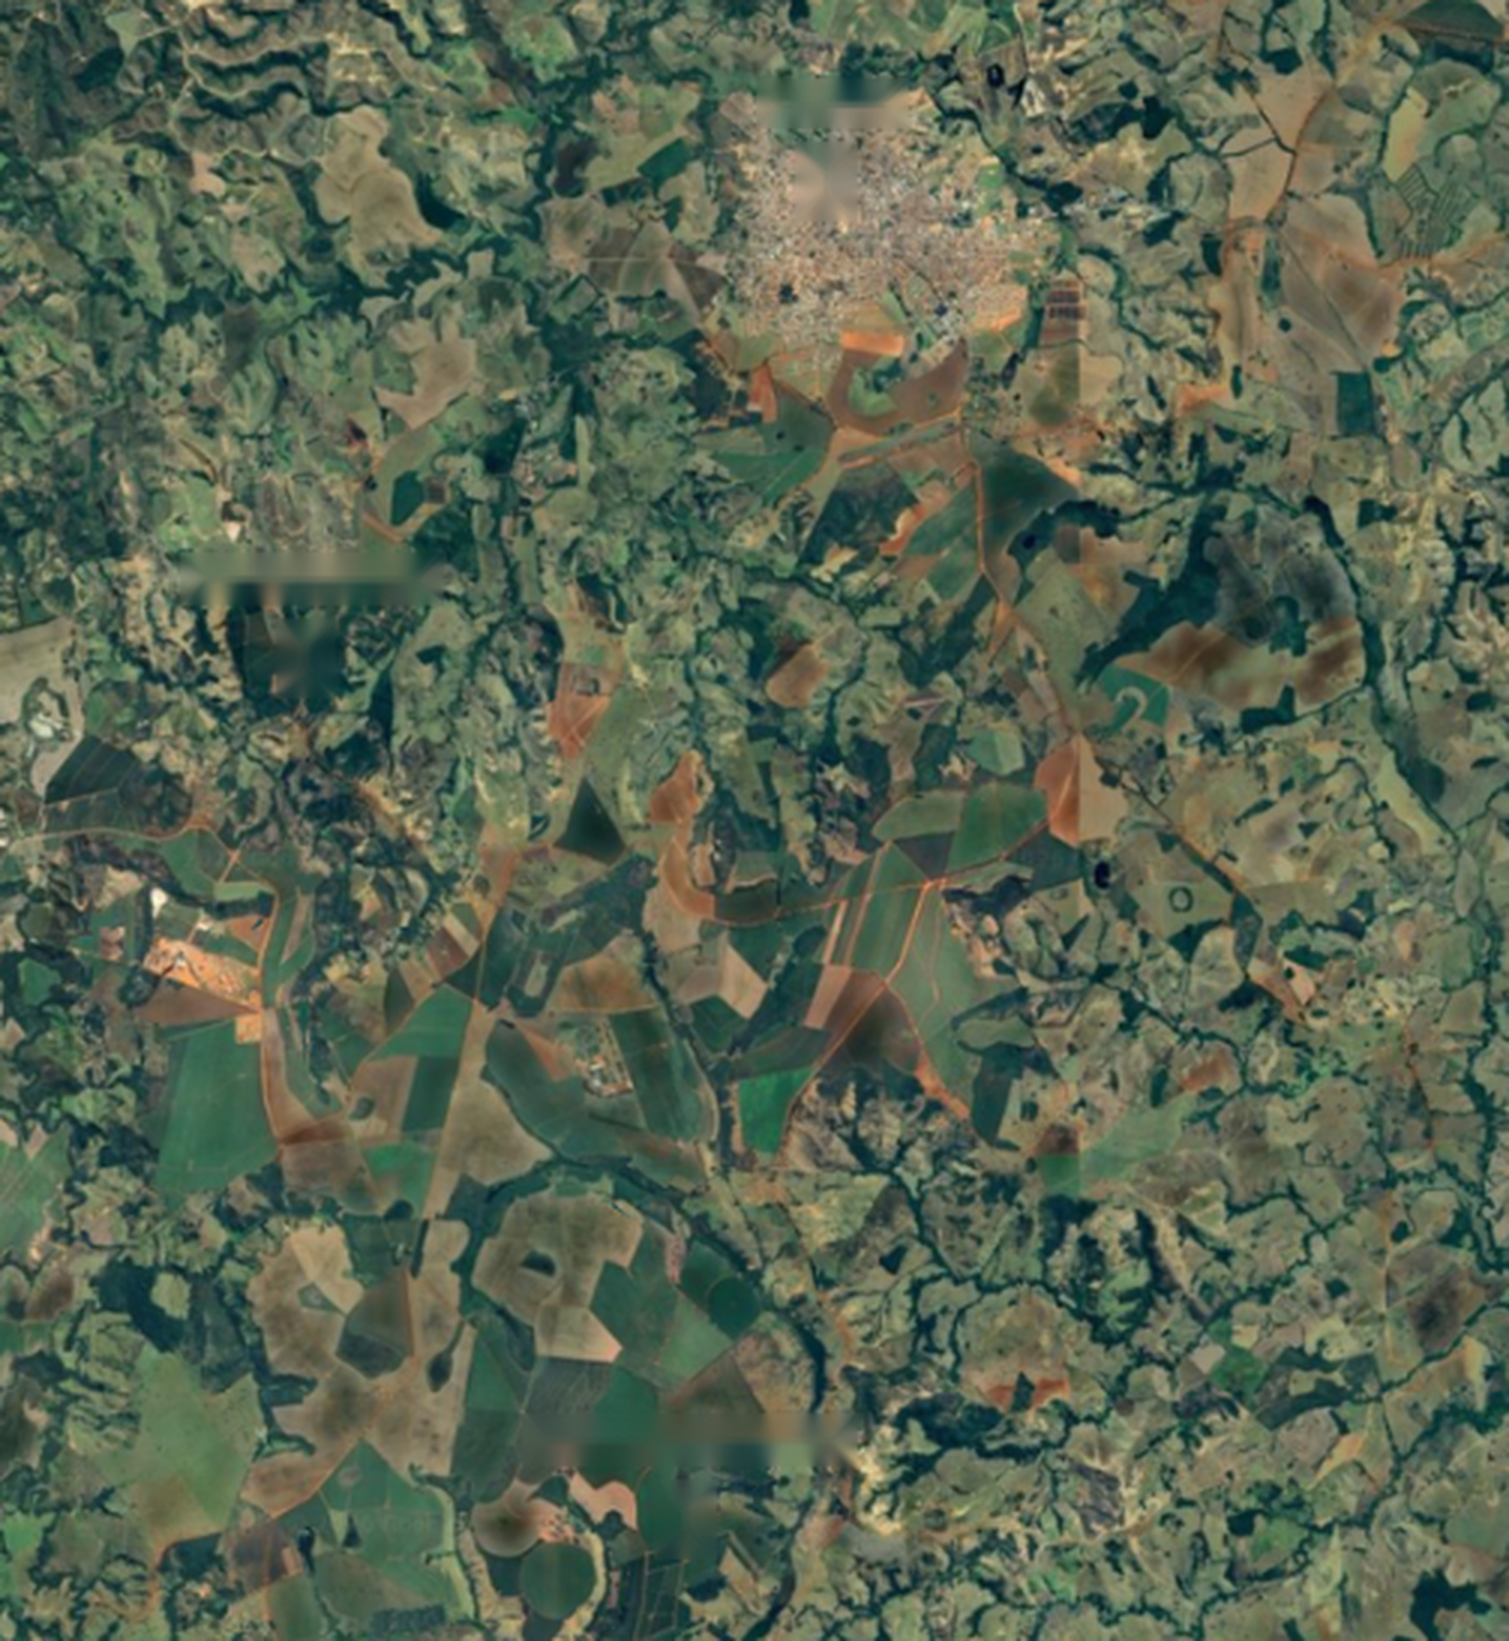
\includegraphics[width=8.40cm]{figuras/mapa/mapa_limpo.png}};

    % alfinetes: disco sobre o ponto, com haste apontando a posição exata
    \foreach \px/\py in {4.601/7.899, 1.703/5.244, 3.816/0.451}{%
        \fill[marca] (\px,\py) -- ++(-0.105,0.27) -- ++(0.21,0) -- cycle;
        \filldraw[marca] (\px,{\py+0.29}) circle (0.16);
        \fill[white] (\px,{\py+0.29}) circle (0.055);
    }

    % rótulos dos sítios
    \node[placa] at (4.634,8.559) {Bambuí};
    \node[placa] at (1.737,5.912) {Fazenda Trevo};
    \node[placa] at (3.841,1.119) {Fazenda do Lazinho};

    \node[letra] at (0.10,9.03) {a};

    % ------------------------------------------------ (b) e (c) fotos
    \node[anchor=north west, inner sep=0] (fb) at (8.62,9.135)
        {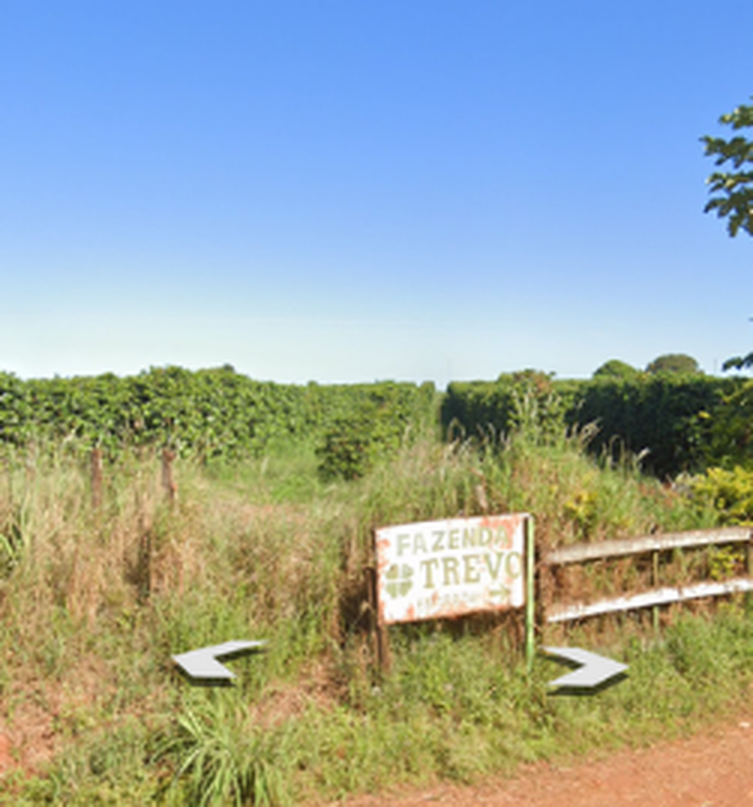
\includegraphics[width=4.18cm]{figuras/mapa/foto_placa.png}};
    \node[anchor=north west, inner sep=0] (fc) at (8.62,4.49)
        {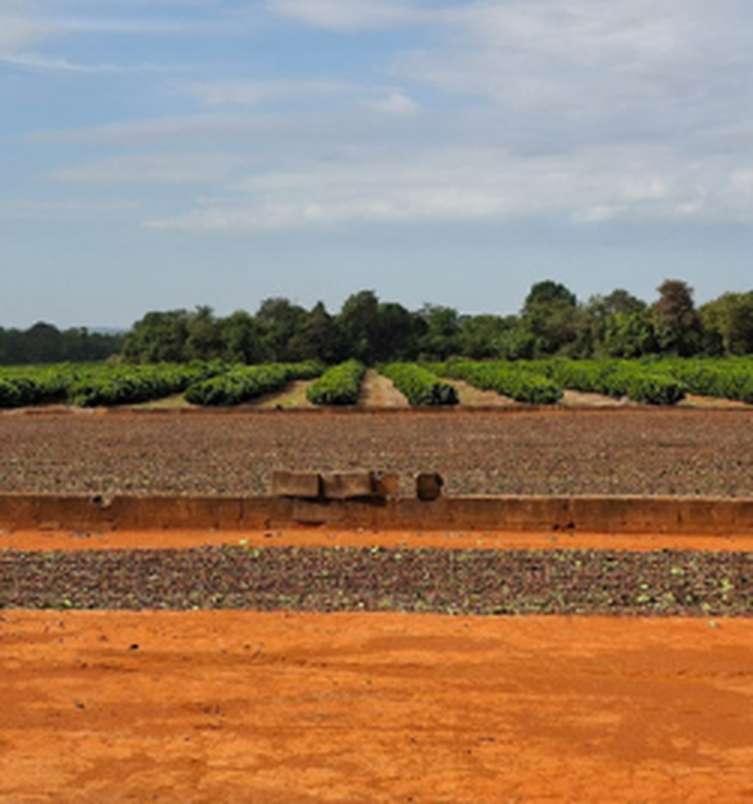
\includegraphics[width=4.18cm]{figuras/mapa/foto_lavoura.png}};

    \node[letra] at ([shift={(0.07,-0.07)}]fb.north west) {b};
    \node[letra] at ([shift={(0.07,-0.07)}]fc.north west) {c};

    \end{tikzpicture}

    \legend{Elaborada pela autora (2026), sobre imagem de satélite do
            Google Earth.}
\end{figure}


O conjunto bruto foi composto por aproximadamente 5.000 imagens contendo frutos das cultivares vermelha e amarela. Após as etapas de anotação, validação estrutural e curadoria das imagens, o conjunto passou por um processo de eliminação de amostras redundantes utilizando o algoritmo \textit{Perceptual Hashing} (pHash), resultando em um conjunto final composto por 2.168 imagens únicas destinadas às etapas experimentais da pesquisa.

Posteriormente, as imagens foram organizadas em subconjuntos destinados ao treinamento, validação e teste dos modelos, mantendo uma divisão fixa ao longo de todos os experimentos realizados neste trabalho.

\begin{figure}[H]
    \centering
    \caption{Exemplos de imagens utilizadas na construção do conjunto de dados, obtidas em diferentes lavouras cafeeiras e condições de aquisição}
    \label{fig:dataset_bruto}
    \figuraMedia{figuras/exemplos_dataset_mosaico_sem_legendas.png}
    \legend{Elaborada pela autora (2026).}
\end{figure}

A Figura~\ref{fig:dataset_bruto} apresenta exemplos representativos das imagens obtidas durante a etapa de aquisição. As amostras ilustram diferentes cenários encontrados em lavouras cafeeiras, incluindo variações na densidade de frutos, condições de iluminação, níveis de oclusão e estágios de maturação. Essa diversidade busca aproximar o conjunto de dados das condições observadas em aplicações reais, contribuindo para o desenvolvimento de modelos com maior capacidade de generalização.

\subsection{Anotação e Organização dos Dados}
\label{sec:anotacao}

Concluída a etapa de aquisição, as imagens foram organizadas e submetidas ao processo de anotação manual, etapa responsável por definir as regiões de interesse utilizadas durante o treinamento supervisionado dos modelos de detecção.

As anotações foram realizadas utilizando a plataforma MakeSense.ai \cite{Makesense2024}. Inicialmente, os rótulos foram produzidos no formato COCO JSON, adotado durante as primeiras etapas do projeto de iniciação científica. Posteriormente, todo o conjunto foi convertido para o formato YOLO, utilizado pela biblioteca Ultralytics e empregado nos experimentos desenvolvidos neste trabalho.

Durante o processo de construção do conjunto de dados foram consideradas duas estratégias de anotação. A primeira utilizou duas classes distintas, correspondentes aos frutos vermelhos e amarelos. Na segunda estratégia, adotada para os experimentos de detecção, todos os frutos passaram a ser representados por uma única classe denominada ``frutos''. Essa abordagem permite concentrar o modelo na localização dos frutos, deixando a classificação do estágio de maturação para uma etapa posterior da pesquisa. A Figura~\ref{fig:anotacao} apresenta um exemplo de imagem do conjunto com as caixas resultantes da anotação manual, e a Figura~\ref{fig:comparacao_classes} compara as duas estratégias.

\begin{figure}[H]
    \centering
    \caption{Exemplo de imagem do conjunto com as caixas delimitadoras anotadas}
    \label{fig:anotacao}
    \figuraVertical{figuras/exemplo_anotacao.jpg}
    \legend{Elaborada pela autora (2026), a partir da imagem \texttt{train\_1048} do subconjunto de treinamento.}
\end{figure}

\begin{figure}[H]
    \centering
    \caption{Comparação entre as estratégias de anotação utilizadas no conjunto de dados}
    \label{fig:comparacao_classes}
    \figuraHorizontal{figuras/comparacao_classes.png}
    \legend{Elaborada pela autora (2026).}
\end{figure}

Após a conclusão das anotações, foi realizada uma etapa de validação automática desenvolvida em Python com o objetivo de verificar a consistência estrutural do conjunto de dados. Os \textit{scripts} implementados permitiram identificar imagens sem arquivos de anotação correspondentes, arquivos vazios, inconsistências no formato YOLO e possíveis incompatibilidades entre imagens e rótulos.

Concluída essa etapa, o conjunto passou por uma curadoria baseada no algoritmo pHash, responsável pela identificação de imagens visualmente semelhantes. Como resultado, foram removidas amostras redundantes preservando apenas uma representação de cada grupo de imagens similares.

Após a curadoria por similaridade visual, o conjunto foi ainda submetido a um
procedimento de revisão do critério de anotação, detalhado na
Subseção~\ref{sec:preprocessamento}. Os valores apresentados a seguir
correspondem à versão consolidada do conjunto de dados, posterior a esse
procedimento. A Tabela~\ref{tab:distribuicao_dataset} apresenta a distribuição final das imagens entre os subconjuntos de treinamento, validação e teste após todas as etapas de validação e curadoria.

\begin{table}[H]
\centering
\caption{Distribuição das imagens e dos arquivos de rótulo entre os subconjuntos após a curadoria e a reanotação}
\label{tab:distribuicao_dataset}
\begin{tabular}{lccc}
\toprule
\textbf{Subconjunto} & \textbf{Imagens} & \textbf{Rótulos} & \textbf{Percentual} \\
\midrule
Treinamento & 1.410 & 1.410 & 65,04\% \\
Validação   & 473   & 473   & 21,82\% \\
Teste       & 285   & 285   & 13,15\% \\
\midrule
Total       & 2.168 & 2.168 & 100,00\% \\
\bottomrule
\end{tabular}
\legend{Elaborada pela autora (2026).}
\end{table}

Após a redistribuição do conjunto de dados, foi realizada uma nova verificação utilizando o algoritmo pHash, com o objetivo de identificar imagens visualmente semelhantes entre os subconjuntos de treinamento, validação e teste. A verificação percorreu as três combinações possíveis, comparando cada uma das 1.410 imagens de treinamento com as 473 de validação e as 285 de teste, e estas últimas entre si, o que totaliza 1.203.585 comparações sob o mesmo limiar de 90\% adotado na curadoria. Nenhum par atingiu o limiar, o que afasta a ocorrência de vazamento de dados (\textit{data leakage}) por imagens visualmente semelhantes em partições distintas.

\begin{figure}[H]
    \centering
    \caption{Distribuição das imagens entre os conjuntos de treinamento, validação e teste}
    \label{fig:distribuicao_particoes}
    \figuraHorizontal{figuras/distribuicao_particoes.pdf}
    \legend{Elaborada pela autora (2026).}
\end{figure}

A Tabela~\ref{tab:distribuicao_dataset} e a Figura~\ref{fig:distribuicao_particoes}
apresentam a distribuição final das imagens e dos arquivos de rótulo entre os
conjuntos de treinamento, validação e teste, após as etapas de curadoria por
pHash e de reanotação descritas na Subseção~\ref{sec:preprocessamento}. O
conjunto final foi composto por 2.168 imagens e 2.168 arquivos de rótulo,
distribuídos nas proporções de aproximadamente 65\%, 22\% e 13\%. O conjunto de
treinamento concentrou 1.410 imagens e 1.410 arquivos de rótulo, enquanto os
conjuntos de validação e teste foram compostos por 473 e 285 imagens e
respectivos arquivos de rótulo. Essa divisão foi mantida fixa durante todos os
experimentos realizados. Para a etapa de detecção de objetos, foi adotada uma
única classe, cuja finalidade é localizar automaticamente os frutos
presentes nas imagens. A classificação do estágio de maturação dos frutos
detectados não integra o escopo deste trabalho e é retomada entre as possibilidades
de continuidade apresentadas na Seção~\ref{sec:conclusao}.

\subsection{Pré-processamento dos Dados}
\label{sec:preprocessamento}

Antes do treinamento dos modelos, foi realizado um conjunto de procedimentos de pré-processamento com o objetivo de garantir a consistência estrutural do conjunto de dados e reduzir fatores que poderiam comprometer a qualidade do treinamento e da avaliação experimental. Essa etapa compreendeu a validação automática das anotações, a reorganização do conjunto de dados, a identificação de imagens redundantes por meio do algoritmo \textit{Perceptual Hashing} (pHash) e a definição das estratégias de aumento artificial de dados empregadas durante o treinamento.

Inicialmente, foram desenvolvidos \textit{scripts} em linguagem Python para verificar automaticamente a integridade das imagens e dos respectivos arquivos de anotação. Esse procedimento permitiu identificar imagens sem arquivos de rótulo correspondentes, arquivos vazios, inconsistências na estrutura das anotações e incompatibilidades entre imagens e respectivos arquivos de anotação. Também foram verificadas as coordenadas normalizadas das caixas delimitadoras, assegurando que todos os valores permanecessem dentro do intervalo estabelecido pelo formato YOLO. As amostras que apresentaram inconsistências foram removidas do conjunto principal e armazenadas separadamente para fins de rastreabilidade e auditoria do processo de construção do conjunto de dados.

Concluída a validação, o conjunto de dados foi reorganizado por meio de uma nova
divisão entre os subconjuntos de treinamento, validação e teste. Durante essa
reorganização foram realizadas verificações para assegurar que uma mesma imagem
não estivesse presente em mais de um subconjunto, preservando a independência
entre as partições utilizadas ao longo dos experimentos.

Além da validação estrutural, foi realizada uma etapa de curadoria destinada à identificação de imagens visualmente redundantes. Embora diferentes arquivos possam possuir nomes distintos, imagens adquiridas em sequência frequentemente representam a mesma cena, reduzindo a variabilidade efetiva do conjunto de treinamento e favorecendo a ocorrência de sobreajuste dos modelos.

Para minimizar esse problema, foi empregado o algoritmo \textit{Perceptual Hashing} (pHash), capaz de representar cada imagem por meio de uma assinatura perceptual baseada em suas características visuais. Inicialmente, as imagens foram convertidas para escala de cinza e redimensionadas para uma resolução padronizada. Em seguida, foi aplicada a \ac{DCT}, utilizando-se as componentes de baixa frequência para a geração do \textit{hash} perceptual. A similaridade entre as imagens foi então determinada por meio da distância de Hamming entre os respectivos \textit{hashes}. A Figura~\ref{fig:fluxo_phash} resume o fluxo adotado para identificação de imagens redundantes utilizando o algoritmo pHash.

\begin{figure}[H]
\centering
\caption{Fluxo de processamento utilizado para cálculo do pHash e identificação de imagens redundantes}
\label{fig:fluxo_phash}

\resizebox{0.94\textwidth}{!}{%
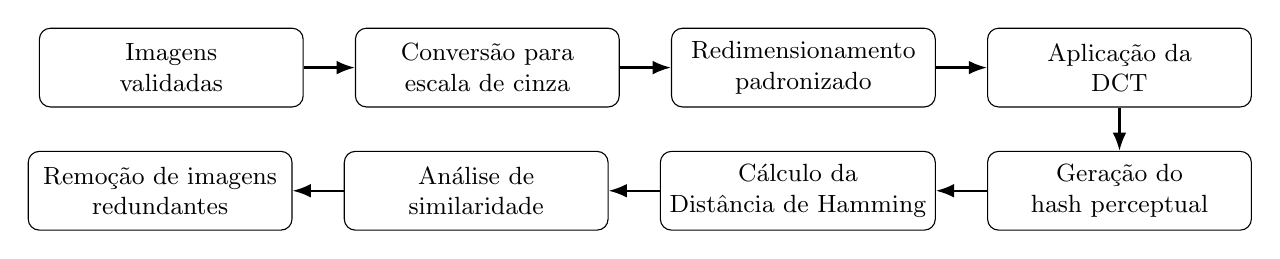
\begin{tikzpicture}[
node distance=0.55cm and 0.65cm,
bloco/.style={
rectangle,
draw,
rounded corners,
align=center,
minimum width=3.35cm,
minimum height=1.0cm,
font=\small
},
seta/.style={-Latex, thick}
]

\node[bloco] (entrada) {Imagens\\validadas};
\node[bloco, right=of entrada] (cinza) {Conversão para\\escala de cinza};
\node[bloco, right=of cinza] (resize) {Redimensionamento\\padronizado};
\node[bloco, right=of resize] (dct) {Aplicação da\\DCT};

\node[bloco, below=of dct] (hash) {Geração do\\hash perceptual};
\node[bloco, left=of hash] (hamming) {Cálculo da\\Distância de Hamming};
\node[bloco, left=of hamming] (similaridade) {Análise de\\similaridade};
\node[bloco, left=of similaridade] (remocao) {Remoção de imagens\\redundantes};

\draw[seta] (entrada) -- (cinza);
\draw[seta] (cinza) -- (resize);
\draw[seta] (resize) -- (dct);
\draw[seta] (dct) -- (hash);
\draw[seta] (hash) -- (hamming);
\draw[seta] (hamming) -- (similaridade);
\draw[seta] (similaridade) -- (remocao);

\end{tikzpicture}%
}

\legend{Elaborada pela autora (2026).}
\end{figure}

A análise de redundância incidiu sobre as 2.511 imagens que haviam sido anotadas e aprovadas na validação estrutural, e não sobre o conjunto bruto. Para a identificação de imagens redundantes foi adotado um limiar de similaridade de 90\%. Os pares cuja similaridade atingiu ou ultrapassou esse valor foram considerados candidatos à redundância e submetidos à inspeção visual antes da remoção definitiva do conjunto de dados.

O procedimento registrou 426 pares acima do limiar, envolvendo 614 imagens distintas, organizadas em 271 grupos de redundância. Em 412 desses pares a similaridade atingiu 100\%, o que corresponde a assinaturas perceptuais idênticas; os 14 restantes situam-se em 96,88\%, 93,75\% e 90,62\%, valores que decorrem da natureza discreta da distância de Hamming sobre um \textit{hash} de 64~bits. A preservação de uma imagem por grupo corresponde às 343 remoções apresentadas na Tabela~\ref{tab:phash}.

\begin{figure}[H]
\centering
\caption{Distribuição dos pares redundantes segundo as partições de origem das duas imagens}
\label{fig:redundancia_phash}
\figuraHorizontal{figuras/redundancia_phash.pdf}
\legend{Elaborada pela autora (2026).}
\end{figure}

A Figura~\ref{fig:redundancia_phash} distribui esses pares segundo as partições a que pertenciam as duas imagens. Quase metade deles, 195 de 426, associa imagens alocadas em partições distintas, com predomínio da combinação entre treinamento e validação. Como a redundância não se restringia ao interior de cada partição, a remoção das amostras foi acompanhada da redistribuição do conjunto, cuja verificação, apresentada na Subseção~\ref{sec:anotacao}, não identificou similaridade remanescente entre as partições.

\begin{table}[H]
\centering
\caption{Resultado da análise de redundância utilizando pHash}
\label{tab:phash}
\begin{tabular}{lc}
\toprule
\textbf{Descrição} & \textbf{Valor} \\
\midrule
Imagens analisadas & 2.511 \\
Pares duplicados identificados & 426 \\
Imagens removidas & 343 \\
Percentual removido & 13,66\% \\
Imagens mantidas & 2.168 \\
\bottomrule
\end{tabular}
\legend{Elaborada pela autora (2026).}
\end{table}

Os resultados obtidos são apresentados na Tabela~\ref{tab:phash}. Ao todo, foram analisadas 2.511 imagens, sendo identificados 426 pares com elevada similaridade visual. Após inspeção manual, 343 imagens redundantes foram removidas, resultando em um conjunto final composto por 2.168 imagens destinadas às etapas experimentais desta pesquisa.

Concluída a etapa de curadoria, foram definidas as estratégias de aumento artificial de dados empregadas durante o treinamento dos modelos. Diferentemente da geração permanente de novas imagens, as transformações são aplicadas dinamicamente pela biblioteca Ultralytics, ampliando a variabilidade das amostras apresentadas ao modelo sem modificar fisicamente o conjunto de dados.

Entre as transformações consideradas encontram-se ajustes de brilho, saturação e matiz, espelhamento horizontal, pequenas rotações, translações e composição por mosaico (\textit{mosaic augmentation}). Essas operações contribuem para aumentar a capacidade de generalização dos modelos e reduzir efeitos associados ao sobreajuste (\textit{overfitting}) \cite{Shorten2019,Mumuni2022DataAugmentation}.

\subsubsection{Identificação de inconsistências no critério de anotação}

Após a conclusão da curadoria por pHash, foi conduzida uma análise da
distribuição de tamanho das caixas delimitadoras presentes no conjunto de
dados, com o objetivo de verificar a consistência do critério de anotação
adotado. Para cada anotação foi calculada a área normalizada da caixa,
obtida pelo produto entre largura e altura relativas às dimensões da
imagem. A análise considerou 13.310 caixas distribuídas entre as 2.168
imagens do conjunto.

A distribuição obtida apresentou comportamento bimodal, com um grupo
predominante de caixas de área reduzida, com mediana de 0,0109, e um
segundo grupo de caixas de área superior, incluindo registros com
área igual a 1,00, ou seja, correspondentes à totalidade da imagem. O
percentil 99 da distribuição alcançou 0,593 e o desvio padrão observado
foi de 0,1044.

A inspeção visual de amostras estratificadas ao longo das faixas de área
identificou a origem dessa bimodalidade. Verificou-se que o conjunto
reunia duas convenções distintas de anotação, decorrentes das diferentes
etapas em que os rótulos foram produzidos ao longo do projeto de iniciação
científica. Na primeira convenção, cada fruto foi delimitado
individualmente. Na segunda, agrupamentos de frutos localizados em um
mesmo ramo foram delimitados por uma única caixa, abrangendo o conjunto
como um objeto único. Em parte das imagens ambas as convenções coexistiam.

A presença simultânea dessas convenções é inadequada ao treinamento
supervisionado de modelos de detecção com classe única, uma vez que
fornece sinais conflitantes quanto à escala e à extensão espacial
esperadas para o objeto de interesse, comprometendo o ajuste da regressão
das caixas delimitadoras. A triagem automatizada identificou 836 arquivos
de anotação contendo ao menos uma caixa incompatível com a convenção de
delimitação individual.

\subsubsection{Reanotação semi-automática}

Considerando o volume de arquivos afetados, optou-se por uma estratégia de
reanotação assistida por modelo, em substituição à reanotação manual
integral. O procedimento foi estruturado em três etapas.

Na primeira etapa, foi organizado um subconjunto composto exclusivamente
pelos arquivos cuja anotação seguia a convenção de delimitação individual,
preservando a divisão original entre treinamento, validação e teste. Na
segunda etapa, esse subconjunto foi utilizado para treinar um modelo
YOLOv8n auxiliar, empregado posteriormente como mecanismo de sugestão de
anotações. Na terceira etapa, o modelo auxiliar foi aplicado às imagens
sinalizadas, gerando propostas de caixas delimitadoras individuais.

Durante a geração das propostas, as caixas originais compatíveis com a
convenção individual foram preservadas, sendo removidas apenas as
sinalizadas como inconsistentes. Propostas do modelo que apresentaram
sobreposição superior a 0,40 de interseção sobre união em relação a caixas
preservadas foram descartadas, evitando duplicidade de anotação. O
procedimento resultou na preservação de 2.324 caixas originais e na
inclusão de 4.231 caixas propostas pelo modelo auxiliar, distribuídas
entre os 836 arquivos processados. Apenas um arquivo não recebeu qualquer
caixa e foi encaminhado para anotação manual integral.

As anotações resultantes foram submetidas a inspeção visual por amostragem
antes de sua incorporação definitiva ao conjunto de dados. A distribuição
de tamanho das caixas foi então recalculada, conforme apresentado na
Tabela~\ref{tab:distribuicao_bbox}, evidenciando a eliminação dos casos
extremos e a redução da dispersão observada anteriormente.

\begin{table}[H]
\centering
\caption{Distribuição de tamanho das caixas delimitadoras antes e após a reanotação semi-automática}
\label{tab:distribuicao_bbox}
\begin{tabular}{lcc}
\toprule
\textbf{Indicador} & \textbf{Antes} & \textbf{Depois} \\
\midrule
Caixas delimitadoras & 13.310 & 17.659 \\
Mediana da área normalizada & 0,0109 & 0,0124 \\
Desvio padrão & 0,1044 & 0,0465 \\
Percentil 99 & 0,5931 & 0,2033 \\
Área máxima observada & 1,0000 & 0,3928 \\
\bottomrule
\end{tabular}
\legend{Elaborada pela autora (2026).}
\end{table}

Observa-se redução do desvio padrão a aproximadamente 44\% do valor
original e eliminação das caixas correspondentes à totalidade da imagem. O
acréscimo no número total de caixas decorre da substituição de
delimitações agrupadas por delimitações individuais dos frutos que as
compunham. Registra-se como limitação do procedimento a permanência de
casos residuais em que frutos adjacentes ou parcialmente sobrepostos
permaneceram delimitados por uma única caixa, situação em que o modelo
auxiliar não realizou a separação e que não foi corrigida manualmente.

Ao final do pré-processamento, o conjunto de dados encontrava-se validado,
organizado, livre de imagens redundantes e com critério de anotação
uniformizado, estando apto à etapa de treinamento dos modelos de detecção. Os
subconjuntos de treinamento, validação e teste foram mantidos fixos durante
todos os experimentos, assegurando a comparabilidade dos resultados obtidos
entre as diferentes arquiteturas e configurações avaliadas.

\subsection{Ambiente Computacional}

Os experimentos desta pesquisa foram conduzidos em ambiente computacional local, configurado para atender às etapas de pré-processamento do conjunto de dados, treinamento dos modelos, validação, conversão para dispositivos móveis e desenvolvimento da aplicação Android. A utilização de uma infraestrutura dedicada permitiu executar de forma integrada todas as fases do fluxo experimental, reduzindo o tempo de processamento e garantindo maior controle sobre a configuração dos experimentos.

As implementações foram desenvolvidas em linguagem Python, utilizando bibliotecas voltadas para visão computacional, aprendizado profundo e manipulação de dados. O treinamento dos modelos foi realizado com a biblioteca Ultralytics, enquanto a conversão para dispositivos móveis empregou o TensorFlow Lite. Para o desenvolvimento da aplicação Android foi utilizado o \textit{framework} Flutter \cite{Flutter2024}, responsável pela integração dos modelos treinados e pela execução dos experimentos em \textit{smartphones}.

A configuração do ambiente computacional utilizado durante o desenvolvimento desta pesquisa é apresentada no Quadro~\ref{quad:ambiente_computacional}.

\begin{board}[H]
\centering
\caption{Configuração do ambiente computacional utilizado no desenvolvimento do trabalho}
\label{quad:ambiente_computacional}
\begin{tabular}{ll}
\toprule
\textbf{Componente} & \textbf{Especificação} \\
\midrule
Processador & AMD Ryzen 5 5500 (6 núcleos, 12 threads) \\
Memória RAM & 16~GB DDR4 \\
Placa gráfica & NVIDIA GeForce RTX 3060 (8~GB GDDR6) \\
Sistema operacional & Windows 11 Pro 64~bits \\
CUDA & 12.x \\
PyTorch & 2.5.1 \\
Ultralytics \ac{YOLO} & 8.4.36 \\
TensorFlow & 2.19.1 \\
Python & 3.11 \\
Conversão Mobile & \ac{TFLite} \\
Aplicação Android & Flutter \\
\bottomrule
\end{tabular}
\legend{Elaborada pela autora (2026).}
\end{board}

Os experimentos foram executados utilizando uma GPU NVIDIA GeForce RTX 3060 com 8~GB de memória dedicada, responsável por acelerar as etapas de treinamento e validação dos modelos. Essa configuração reduziu o tempo necessário para a realização dos experimentos e possibilitou a avaliação de diferentes combinações de hiperparâmetros durante o processo de desenvolvimento.

Além do treinamento, o ambiente computacional foi empregado na conversão dos modelos para o formato TensorFlow Lite e na geração dos artefatos posteriormente integrados à aplicação Android utilizada na avaliação experimental.

\subsection{Treinamento dos Modelos}

Concluído o pré-processamento do conjunto de dados, iniciou-se a etapa de treinamento dos modelos de detecção de objetos empregados nesta pesquisa. Foram selecionadas duas arquiteturas da família YOLO, YOLOv8n e YOLOv10n, por apresentarem um equilíbrio entre desempenho de detecção e custo computacional, característica relevante para aplicações executadas em dispositivos móveis.

Os modelos foram inicializados a partir de pesos pré-treinados no conjunto de dados \ac{COCO}, empregando a estratégia de \textit{transfer learning} por meio de \textit{fine-tuning} \cite{Tan2023TransferLearning}. Durante o treinamento foi considerada uma única classe denominada ``frutos'', permitindo que os modelos concentrassem o aprendizado na localização dos frutos presentes nas imagens.

Os treinamentos foram conduzidos utilizando a biblioteca Ultralytics YOLO.
Foram adotados tamanho de entrada de 960~$\times$~960~pixels, otimizador
AdamW e taxa de aprendizado inicial de 0,003. O tamanho de lote foi
definido em 8 imagens, em decorrência da capacidade de memória dedicada da
placa gráfica utilizada. Testes preliminares com lotes de 16 imagens
resultaram em esgotamento da memória disponível na unidade de
processamento gráfico durante a etapa de validação, inviabilizando a
execução do treinamento nessa configuração.

Adicionalmente, foram desabilitados o treinamento em precisão mista e o
carregamento paralelo de dados, ajustes necessários para contornar
incompatibilidades observadas entre a biblioteca de aceleração por
hardware e o sistema operacional utilizado. O armazenamento em memória do
conjunto de imagens também foi desabilitado, considerando a capacidade de
memória principal disponível e a resolução das imagens processadas.

As estratégias de aumento artificial de dados descritas na
Subseção~\ref{sec:preprocessamento} foram aplicadas dinamicamente
durante o treinamento, contemplando variações de matiz, saturação e
brilho, espelhamento horizontal, rotações de até cinco graus, translações
de até 10\%, variações de escala e composição por mosaico.

O treinamento do modelo YOLOv10n foi conduzido por 80 épocas. Para o
modelo YOLOv8n, a execução foi encerrada na época 74, uma vez que as
métricas de validação apresentaram estabilização a partir da época 45,
sem tendência de melhoria nas épocas subsequentes. Os pesos
correspondentes ao melhor desempenho no conjunto de validação foram
preservados em ambos os casos, adotando-se a métrica mAP@0,50 como
critério principal de seleção.

\begin{board}[H]
\centering
\caption{Configuração de treinamento adotada nos experimentos}
\label{quad:config_treinamento}
\begin{tabular}{ll}
\toprule
\textbf{Parâmetro} & \textbf{Valor} \\
\midrule
Tamanho de entrada & 960~$\times$~960~pixels \\
Otimizador & AdamW \\
Taxa de aprendizado inicial & 0,003 \\
Fator da taxa final & 0,01, com decaimento linear \\
Decaimento de pesos & 0,0005 \\
Momento & 0,937 \\
Épocas de aquecimento & 3 \\
Tamanho do lote & 8 \\
Épocas configuradas & 120 (YOLOv8n) e 80 (YOLOv10n) \\
Épocas executadas & 74 (YOLOv8n) e 80 (YOLOv10n) \\
Paciência da parada antecipada & 30 épocas \\
Semente & 0, em modo determinístico \\
Pesos iniciais & Pré-treinados em COCO \\
Precisão mista & Desabilitada \\
Classe & ``frutos'' \\
Critério de seleção & mAP@0,50 (validação) \\
\bottomrule
\end{tabular}
\legend{Elaborada pela autora (2026).}
\end{board}

\subsection{Conversão dos Modelos para TFLite}
\label{sec:conversao_tflite}

Concluído o treinamento, os modelos selecionados foram convertidos para o formato \ac{TFLite}. Essa etapa tem como objetivo reduzir os requisitos computacionais necessários para a inferência, possibilitando a execução local dos modelos em \textit{smartphones} Android sem dependência de conexão com serviços externos.

A conversão foi conduzida por meio da biblioteca Ultralytics, que realiza a exportação em etapas encadeadas. Os pesos treinados em PyTorch foram inicialmente convertidos para o formato ONNX (do inglês \textit{Open Neural Network Exchange}), utilizando conjunto de operadores na versão 19. Em seguida, o grafo computacional foi convertido para o formato SavedModel do TensorFlow e, por fim, para o formato \texttt{.tflite}. A resolução de entrada foi mantida em 960~$\times$~960~pixels, correspondente à utilizada durante o treinamento.

Foram geradas três variantes de cada modelo. A versão em \ac{FP32} preserva a precisão numérica original e foi adotada como referência. A versão em \ac{FP16} reduz pela metade a largura de representação dos pesos. A versão em \ac{INT8} aplica quantização pós-treinamento, convertendo pesos e ativações para representação inteira de oito bits. Essas estratégias permitem reduzir o tamanho final dos modelos e, em determinados cenários, melhorar o tempo de inferência e a eficiência energética dos dispositivos móveis \cite{Menghani2023Efficient}.

A quantização \ac{INT8} requer uma etapa adicional de calibração, na qual um conjunto representativo de imagens é processado pelo conversor para determinar as faixas de valores assumidas pelas ativações em cada camada da rede. Para essa finalidade foram utilizadas as 473 imagens do subconjunto de validação, preservando o subconjunto de teste para a avaliação posterior das variantes convertidas.

Os modelos convertidos foram submetidos a testes de integridade funcional, verificando a consistência das predições em relação aos modelos originais treinados no ambiente de desenvolvimento. Para essa finalidade foi utilizado o conjunto de teste, permitindo comparar os resultados produzidos pelas versões originais e convertidas.

Registra-se que os modelos apresentam formatos de saída distintos em decorrência de suas arquiteturas. O YOLOv8n produz um tensor de dimensões (1, 5, 18900), correspondente a candidatos que demandam filtragem por supressão não máxima na aplicação. O YOLOv10n produz um tensor de dimensões (1, 300, 6), contendo até 300 detecções já filtradas, no formato composto por coordenadas da caixa delimitadora, confiança e classe. Essa diferença implica implementações distintas de pós-processamento na aplicação móvel. A Figura~\ref{fig:fluxo_tflite} apresenta o fluxo adotado para conversão, otimização e validação dos modelos destinados à execução em dispositivos Android.

\begin{figure}[H]
\centering
\caption{Fluxo de conversão e otimização dos modelos para TensorFlow Lite}
\label{fig:fluxo_tflite}
\resizebox{0.86\textwidth}{!}{%
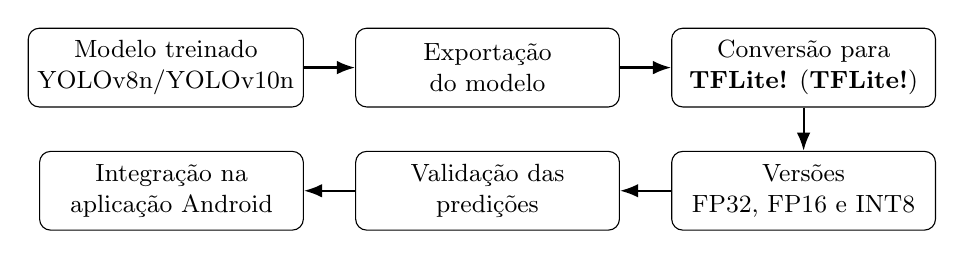
\begin{tikzpicture}[
node distance=0.55cm and 0.65cm,
bloco/.style={
draw,
rounded corners,
align=center,
minimum width=3.35cm,
minimum height=1.0cm,
font=\small
},
seta/.style={-Latex, thick}
]

\node[bloco] (yolo) {Modelo treinado\\YOLOv8n/YOLOv10n};
\node[bloco, right=of yolo] (export) {Exportação\\do modelo};
\node[bloco, right=of export] (convert) {Conversão para\\\ac{TFLite}};

\node[bloco, below=of convert] (quant) {Versões\\FP32, FP16 e INT8};
\node[bloco, left=of quant] (valid) {Validação das\\predições};
\node[bloco, left=of valid] (android) {Integração na\\aplicação Android};

\draw[seta] (yolo) -- (export);
\draw[seta] (export) -- (convert);
\draw[seta] (convert) -- (quant);
\draw[seta] (quant) -- (valid);
\draw[seta] (valid) -- (android);

\end{tikzpicture}%
}
\legend{Elaborada pela autora (2026).}
\end{figure}

\subsection{Aplicação Android}
\label{sec:aplicacao_android}
 
Com o objetivo de avaliar a execução dos modelos em ambiente real de uso, foi
desenvolvida uma aplicação móvel para dispositivos Android utilizando o
\textit{framework} Flutter \cite{Flutter2024}. A aplicação, denominada
CaféScan, realiza o carregamento local dos modelos convertidos para o formato
\ac{TFLite}, executa as inferências diretamente no dispositivo e apresenta
visualmente os resultados da detecção. Todo o processamento ocorre localmente
no \textit{smartphone}, sem dependência de conexão com serviços externos ou
infraestrutura em nuvem.
 
A integração entre a aplicação e os modelos foi realizada por meio da
biblioteca tflite\_flutter, que expõe o interpretador do \ac{TFLite}
ao ambiente de execução do Flutter. As seis variantes geradas na etapa de
conversão foram incorporadas à aplicação, podendo ser selecionadas durante a
execução sem necessidade de reinstalação. A escolha do \textit{delegate} é
igualmente realizada em tempo de execução, no momento da construção do
interpretador, o que permite alternar entre as configurações experimentais de
forma direta.
 
\subsubsection{Preparação das imagens}
 
O pré-processamento reproduz o procedimento adotado durante o treinamento. As
imagens são redimensionadas para 960~$\times$~960~pixels preservando a
proporção original, sendo as margens remanescentes preenchidas com valor
uniforme. Os valores dos canais são normalizados para o intervalo entre zero e
um e organizados em um vetor contíguo de ponto flutuante.
 
A adoção de estrutura contígua para o tensor de entrada mostrou-se necessária
por razões de desempenho. Implementações baseadas em listas aninhadas exigem a
alocação de aproximadamente 2,7 milhões de objetos por imagem na resolução
adotada, o que domina o tempo de processamento em dispositivos móveis. Medições
preliminares indicaram redução superior a 60\% no tempo de preparação após a
substituição da estrutura de dados.
 
\subsubsection{Interpretação das saídas}
 
O tratamento das predições difere conforme a arquitetura, em decorrência dos
formatos de saída descritos na Subseção~\ref{sec:conversao_tflite}.
 
Para o YOLOv8n, cujo tensor de saída contém 18.900 candidatos descritos por
coordenadas e confiança, a aplicação implementa a supressão não máxima. O
procedimento ordena os candidatos por confiança decrescente e descarta aqueles
cuja interseção sobre união com uma detecção previamente aceita excede o limiar
estabelecido. Foram adotados os mesmos limiares empregados na validação em
ambiente de desenvolvimento, assegurando a comparabilidade entre as medições.
 
Para o YOLOv10n, cujo tensor contém até 300 detecções já filtradas pelo próprio
modelo, a aplicação realiza apenas a filtragem por confiança mínima,
dispensando o procedimento de supressão.
 
\subsubsection{Funcionalidades}
 
A aplicação organiza-se em quatro funcionalidades principais, cujas telas constam da Figura~\ref{fig:telas_aplicacao}.
 
A primeira permite selecionar a configuração experimental, combinando uma das
seis variantes de modelo com um dos dois \textit{delegates} disponíveis. A
troca de configuração provoca o recarregamento do interpretador, sendo o estado
apresentado ao usuário por meio de indicador visual.
 
A segunda executa a detecção sobre uma imagem individual, capturada pela câmera
ou selecionada na galeria. Os resultados são apresentados por meio de caixas
delimitadoras sobrepostas à imagem, acompanhadas das respectivas confianças e
da decomposição do tempo de processamento.
 
A terceira realiza a execução em lote sobre um conjunto de imagens, constituindo
o instrumento de coleta das medições experimentais. As primeiras inferências são
executadas sem registro, uma vez que a alocação inicial de recursos pelo
interpretador eleva a latência das primeiras execuções. O
número de inferências descartadas é configurável na própria aplicação.
 
A quarta apresenta as métricas agregadas das execuções realizadas, permitindo a
comparação entre as configurações avaliadas e a exportação dos dados em formato
de valores separados por vírgula, com registro individual por imagem
processada.
 
\begin{figure}[H]
    \centering
    \caption{Telas da aplicação: (a) escolha da configuração experimental;
    (b) detecção sobre imagem individual; (c) execução em lote; (d) métricas
    agregadas das execuções}
    \label{fig:telas_aplicacao}
    \figuraHorizontal{figuras/telas_aplicacao.jpg}
    \legend{Elaborada pela autora (2026), a partir de capturas de tela do
    aparelho descrito na Subseção~\ref{sec:dispositivo}.}
\end{figure}

\subsubsection{Métricas coletadas}
 
Durante a execução em lote, a aplicação registra, para cada imagem, o tempo de
preparação da imagem, o tempo de inferência, o tempo de interpretação das
saídas, o número de detecções obtidas e o consumo de memória residente do
processo. O nível de carga da bateria é registrado no início e ao final de cada
execução.
 
A decomposição do tempo em três etapas permite distinguir o custo atribuível ao
modelo daquele decorrente das operações auxiliares realizadas pela aplicação.
Uma vez que a preparação das imagens é idêntica em todas as configurações
avaliadas, o tempo de inferência constitui a medida adequada para a comparação
entre modelos, estratégias de quantização e \textit{delegates}.
 
A partir dos registros individuais são calculadas a média, o desvio padrão
amostral e o coeficiente de variação da latência. Este último foi adotado por
permitir comparar a estabilidade entre configurações com latências médias
distintas, situação em que o desvio padrão absoluto tende a acompanhar a
magnitude da medida.
 
Registra-se que a temperatura do dispositivo não pôde ser incorporada ao
conjunto de métricas coletadas automaticamente. As interfaces de acesso a
sensores térmicos no sistema Android requerem permissões de nível privilegiado,
não disponíveis a aplicações comuns, e não são expostas pelo \textit{framework}
utilizado.
 
\subsection{Dispositivo de Avaliação}
\label{sec:dispositivo}
 
As medições foram conduzidas em um aparelho Samsung Galaxy S24
(SM-S921B), equipado com o \ac{SoC} Exynos 2400, de fabricação
própria da Samsung, unidade gráfica Xclipse 940, baseada na
arquitetura RDNA da AMD, 8~GB de memória principal e sistema
operacional Android~16. A identificação do fornecedor da unidade
gráfica é relevante para a leitura dos resultados, uma vez que o
suporte a operações do \textit{delegate} \ac{GPU} do \ac{TFLite}
é implementado por fornecedor.
 
A escolha do aparelho não decorreu de amostragem, mas de
disponibilidade, uma vez que se trata do dispositivo pessoal da
autora, único disponível durante a janela de coleta. Essa circunstância constitui
limitação relevante e condiciona a leitura dos resultados.
 
O Galaxy S24 situa-se no segmento superior do mercado, ao passo que a
aplicação proposta destina-se ao uso em campo por produtores, contexto em
que predominam aparelhos de entrada e intermediários. As latências aqui
reportadas devem, portanto, ser interpretadas como limite inferior do que
se observaria naquele contexto. Mais importante, a disponibilidade e o
comportamento dos \textit{delegates} variam conforme o fornecedor do
\textit{chipset} e a versão do \textit{driver} gráfico, de modo que os resultados
relativos entre \textit{delegates} não são diretamente transferíveis a outras
plataformas de \textit{hardware}.
 
Essa limitação é retomada na Subseção~\ref{sec:limitacoes}, onde se discute
sua extensão, e orienta a proposta de ampliação da avaliação a
dispositivos adicionais, registrada entre os trabalhos futuros.

\subsection{Avaliação Experimental}
\label{sec:avaliacao_experimental}

A etapa de avaliação experimental foi concebida para analisar o comportamento dos modelos de detecção em condições próximas às encontradas em aplicações reais. Diferentemente da avaliação realizada apenas em ambiente de treinamento, os experimentos desta pesquisa buscam investigar o impacto conjunto da arquitetura do modelo, da estratégia de quantização e do mecanismo de aceleração por \textit{hardware} sobre o desempenho da inferência em dispositivos Android.

Para essa finalidade, foram avaliadas as arquiteturas YOLOv8n e YOLOv10n convertidas para o formato \ac{TFLite}, considerando diferentes configurações de quantização (\ac{FP32}, \ac{FP16} e \ac{INT8}) e os \textit{delegates} de \ac{CPU} e \ac{GPU} disponibilizados pela plataforma. Essa combinação permite analisar o equilíbrio entre qualidade da detecção e custo computacional em diferentes cenários de execução.

Os experimentos foram conduzidos no dispositivo descrito na Subseção~\ref{sec:dispositivo}. Antes de cada execução o aparelho foi configurado com brilho fixo da tela, modo de economia de energia desativado e aplicações em segundo plano encerradas. O nível de carga no início das execuções variou entre 49\% e 94\%, não tendo sido mantido acima de um limiar fixo; essa variação constitui limitação do protocolo, registrada na Subseção~\ref{sec:limitacoes}. A avaliação em dispositivos de diferentes faixas de desempenho permanece como possibilidade de continuidade.

Para cada combinação de modelo, estratégia de quantização e \textit{delegate},
foram realizadas inferências sobre as 285 imagens pertencentes ao conjunto de
teste, precedidas de dez inferências de aquecimento descartadas da apuração.
Cada configuração foi executada uma única vez. A ausência de repetições impede
separar a variabilidade atribuível ao sistema operacional daquela própria da
configuração avaliada, e está registrada entre as limitações do estudo.

As métricas analisadas foram organizadas em dois grupos complementares. O primeiro grupo contempla indicadores relacionados à qualidade da detecção, incluindo \ac{mAP}@0,50, precisão e revocação. O segundo grupo reúne métricas voltadas ao desempenho computacional da inferência móvel, incluindo tempo médio de inferência, \ac{FPS}, consumo de memória \ac{RAM} e consumo energético.

A coleta dessas métricas foi realizada diretamente pela aplicação Android desenvolvida nesta pesquisa. Informações relacionadas ao consumo energético e à utilização de recursos computacionais foram obtidas por meio das APIs disponibilizadas pelo sistema operacional Android, incluindo a interface BatteryManager.

Os resultados obtidos foram organizados em tabelas e gráficos comparativos, de modo a permitir a análise simultânea do desempenho da detecção e do custo computacional associado a cada configuração experimental, e a identificação da combinação que oferece o melhor equilíbrio entre qualidade da detecção, latência e estabilidade de execução em dispositivos móveis.

\begin{board}[H]
\centering
\caption{Configurações avaliadas experimentalmente}
\label{quad:configuracoes_experimentos}
\begin{tabular}{cccc}
\toprule
Modelo & Quantização & \textit{Delegate} & Situação \\
\midrule
YOLOv8n & FP32 & CPU & Executada \\
YOLOv8n & FP16 & CPU & Executada \\
YOLOv8n & INT8 & CPU & Executada \\
YOLOv8n & FP32 & GPU & Executada \\
YOLOv8n & FP16 & GPU & Executada \\
YOLOv8n & INT8 & GPU & Executada \\
YOLOv10n & FP32 & CPU & Executada \\
YOLOv10n & FP16 & CPU & Executada \\
YOLOv10n & INT8 & CPU & Executada \\
YOLOv10n & FP32 & GPU & Executada \\
YOLOv10n & FP16 & GPU & Executada \\
YOLOv10n & INT8 & GPU & Não executável \\
\bottomrule
\end{tabular}
\legend{Elaborada pela autora (2026).}
\end{board}

O Quadro~\ref{quad:configuracoes_experimentos} resume todas as combinações de arquitetura, estratégia de quantização e \textit{delegate} consideradas na avaliação experimental. A combinação YOLOv10n/\ac{INT8}/\ac{GPU} não é executável, pois as operações exigidas pela arquitetura não são suportadas pelo \textit{delegate} \ac{GPU}, conforme discutido na Subseção~\ref{sec:v10n_gpu}. A comparação entre as demais permite identificar o impacto individual e combinado de cada fator sobre o desempenho dos modelos executados em \textit{smartphones} Android.

\subsection{Coleta em Múltiplos Dispositivos}
\label{sec:coleta_multidispositivo}

A disponibilidade e o comportamento dos \textit{delegates} dependem do
fornecedor do \ac{SoC} e da versão do \textit{driver} gráfico, de modo que
medições obtidas em um único aparelho não se transferem a outras plataformas
sem verificação. Para examinar se as diferenças observadas entre configurações
se mantêm fora do aparelho descrito na Subseção~\ref{sec:dispositivo}, a
aplicação foi distribuída a voluntários e executada em aparelhos de
fabricantes, faixas de preço e versões de sistema distintas.

O arquivo de instalação é o mesmo em todos os aparelhos, inclusive no de
referência, de modo que nenhuma diferença entre as medições decorre da versão
da aplicação. Os modelos convertidos acompanham esse arquivo e não são obtidos
pela rede, o que mantém idênticos também os pesos executados.

Medir as 285 imagens da partição de teste em doze configurações exigiria de
cada voluntário tempo incompatível com uma contribuição espontânea. Foi
definido um subconjunto de 30 imagens da mesma partição, que abrange de 1,2 a
16,1~megapixels e de 1 a 45 caixas anotadas, perfazendo 271 instâncias, e que
preserva a faixa de resolução e de densidade de anotação do conjunto completo.
As mesmas 30 imagens, nos arquivos originais, foram distribuídas junto com a
aplicação.

O protocolo entregue aos voluntários requer carga acima de 80\% e fora do
carregador, aparelho em repouso térmico, aplicações em segundo plano
encerradas e aplicação em primeiro plano durante toda a execução. Cada
configuração é precedida de dez inferências de aquecimento descartadas da
apuração, como na avaliação do aparelho de referência.

A aplicação executa as doze configurações em sequência, sem intervenção entre
elas, e grava ao final um arquivo por configuração. Cada arquivo registra o
fabricante, o modelo, o identificador do \textit{hardware}, a versão do
Android, o nível de carga no início e no fim da execução e as medições
individuais por imagem, o que permite verificar o cumprimento do protocolo a
partir dos próprios dados, sem depender do relato de quem executou.

No aparelho de referência a varredura foi repetida em três sessões realizadas
na mesma noite, com intervalos de 40 e 46~minutos entre elas e carga entre
99\% e 83\%, com a finalidade de estimar a variação entre execuções de uma
mesma configuração.

\subsection{Métricas de Avaliação}

A comparação entre as diferentes configurações dos modelos foi realizada por meio de métricas relacionadas à qualidade da detecção e ao desempenho computacional durante a execução em dispositivos móveis. A utilização desses dois grupos de indicadores permite avaliar não apenas a capacidade dos modelos em detectar corretamente os frutos de café, mas também sua viabilidade para aplicações embarcadas em \textit{smartphones} Android. O Quadro~\ref{quad:metricas_avaliacao} apresenta um resumo das métricas consideradas nesta pesquisa, bem como suas respectivas unidades de medida e finalidade na avaliação experimental.

\begin{board}[H]
\centering
\caption{Métricas utilizadas na avaliação experimental}
\label{quad:metricas_avaliacao}
\small
\begin{tabularx}{\textwidth}{p{2.6cm}p{3.0cm}p{2.2cm}X}
\toprule
\textbf{Grupo} & \textbf{Métrica} & \textbf{Unidade} & \textbf{Objetivo} \\
\midrule
Detecção & \ac{mAP}@0,50 & \% & Avaliar o desempenho geral da detecção \\
Detecção & Precisão & \% & Quantificar a proporção de detecções corretas \\
Detecção & Revocação & \% & Medir a capacidade de localizar os objetos presentes \\
Computacional & Tempo de inferência & ms & Avaliar a latência da inferência \\
Computacional & \ac{FPS} & quadros/s & Medir a taxa de processamento das imagens \\
Computacional & Memória \ac{RAM} & MB & Quantificar o consumo de memória \\
Computacional & Consumo energético & \% & Avaliar o impacto energético da inferência \\
Computacional & Estabilidade & \% & Avaliar a consistência entre inferências consecutivas, pelo coeficiente de variação \\
\bottomrule
\end{tabularx}
\legend{Elaborada pela autora (2026).}
\end{board}

As métricas de qualidade da detecção compreendem o \ac{mAP}@0,50, a precisão e a revocação, calculadas a partir do conjunto de teste. O \ac{mAP}@0,50 foi adotado como principal indicador de desempenho, por sintetizar simultaneamente a capacidade de localização e classificação dos objetos detectados. As métricas de precisão e revocação foram utilizadas de forma complementar para analisar, respectivamente, a proporção de detecções corretas e a capacidade do modelo em localizar os frutos presentes nas imagens.

As métricas relacionadas ao desempenho computacional incluem o tempo médio de inferência, a taxa de processamento em quadros por segundo (\ac{FPS}), o consumo de memória \ac{RAM}, o consumo energético e a estabilidade da execução. Esses indicadores permitem caracterizar o custo computacional imposto por cada configuração avaliada e analisar sua adequação para execução em dispositivos móveis.

A estabilidade foi avaliada por meio da variabilidade observada entre inferências consecutivas realizadas sob as mesmas condições experimentais. Adotou-se o coeficiente de variação, razão entre o desvio padrão e a média, por permitir a comparação entre configurações cujas latências médias diferem em uma ordem de grandeza, situação em que o desvio padrão absoluto acompanha a magnitude da medida. Valores reduzidos indicam maior consistência entre as execuções, ao passo que valores elevados apontam oscilações decorrentes da arquitetura do modelo, da estratégia de quantização ou do mecanismo de aceleração utilizado.

As métricas de precisão e revocação são calculadas a partir das quantidades de verdadeiros positivos (TP, do inglês \textit{True Positives}), falsos positivos (FP, do inglês \textit{False Positives}) e falsos negativos (FN, do inglês \textit{False Negatives}), conforme apresentado nas Equações~\ref{eq:precision} e~\ref{eq:recall}.

\begin{equation}
\label{eq:precision}
P=\frac{TP}{TP+FP}
\end{equation}

em que $TP$ representa o número de verdadeiros positivos e $FP$ o número de falsos positivos.

\begin{equation}
\label{eq:recall}
R=\frac{TP}{TP+FN}
\end{equation}

em que $FN$ representa o número de falsos negativos.

O \ac{mAP}@0,50 corresponde à média das precisões médias calculadas considerando um limiar de interseção sobre união (IoU, do inglês \textit{Intersection over Union}) igual a 0,50. Essa métrica sintetiza simultaneamente a capacidade de localização e classificação dos objetos detectados, sendo utilizada como principal critério para comparação entre os modelos avaliados.

A taxa de processamento em quadros por segundo (\ac{FPS}) é obtida a partir da latência total por imagem, que compreende o pré-processamento, a inferência e o pós-processamento, conforme apresentado na Equação~\ref{eq:fps}. Adota-se a latência total, e não a de inferência isolada, por corresponder à taxa efetivamente percebida pelo usuário da aplicação.

\begin{equation}
\label{eq:fps}
FPS=\frac{1000}{T_{\mathrm{total}}}
\end{equation}

em que $T_{\mathrm{total}}$ representa a latência total média por imagem, expressa em milissegundos. Valores mais elevados de \ac{FPS} indicam maior capacidade de processamento em tempo real.

O desvio padrão amostral das medições, base do coeficiente de variação, foi calculado de acordo com a Equação~\ref{eq:desvio}.

\begin{equation}
\label{eq:desvio}
\sigma=\sqrt{\frac{\sum_{i=1}^{n}(x_i-\bar{x})^2}{n-1}}
\end{equation}

em que $x_i$ representa cada medição individual, $\bar{x}$ corresponde à média das medições e $n$ representa o número total de observações. Valores reduzidos de $\sigma$ indicam maior estabilidade entre inferências consecutivas.

Em conjunto, essas métricas permitirão analisar simultaneamente a qualidade da detecção, o desempenho computacional e a estabilidade dos modelos executados em dispositivos Android, possibilitando identificar as configurações que apresentam o melhor equilíbrio entre acurácia, velocidade de inferência e eficiência computacional.

\section{RESULTADOS}
\label{sec:resultados}

Esta seção apresenta os resultados obtidos, contemplando a caracterização do
conjunto de dados construído, os procedimentos de anotação e curadoria, o
desempenho dos modelos de detecção treinados, a conversão para \ac{TFLite} e a
avaliação experimental em dispositivo Android.

\subsection{Caracterização do Conjunto de Dados}

A etapa de aquisição resultou em um conjunto bruto de aproximadamente 5.000
imagens obtidas em lavouras cafeeiras localizadas no município de Bambuí, Minas
Gerais. As imagens foram capturadas em condições reais de campo, contemplando
diferentes condições de iluminação, níveis de oclusão dos frutos, densidades de
vegetação e perspectivas de aquisição. A Figura~\ref{fig:mapa_bambui} apresenta
a localização da área utilizada para a coleta e a
Figura~\ref{fig:dataset_bruto} apresenta exemplos representativos das imagens
obtidas.

Do conjunto bruto, 2.511 imagens foram anotadas e submetidas à validação
estrutural. A curadoria por pHash identificou e removeu 343 imagens
redundantes, resultando em 2.168 imagens únicas destinadas aos experimentos.
Registra-se que aproximadamente metade do conjunto bruto permanece sem
anotação, constituindo possibilidade de ampliação futura da base. A Tabela~\ref{tab:estatisticas_dataset} apresenta um resumo das características
do conjunto de dados efetivamente utilizado nos experimentos.

\begin{table}[H]
\centering
\caption{Resumo das características do conjunto de dados utilizado nos experimentos}
\label{tab:estatisticas_dataset}
\begin{tabular}{lc}
\toprule
\textbf{Característica} & \textbf{Valor} \\
\midrule
Imagens coletadas (conjunto bruto) & $\approx$ 5.000 \\
Imagens anotadas e validadas & 2.511 \\
Imagens removidas por pHash & 343 \\
Imagens finais & 2.168 \\
Imagens de treinamento & 1.410 \\
Imagens de validação & 473 \\
Imagens de teste & 285 \\
Instâncias anotadas (total) & 17.659 \\
Instâncias anotadas (treinamento) & 11.288 \\
Instâncias anotadas (validação) & 3.972 \\
Instâncias anotadas (teste) & 2.399 \\
Classes & 1 \\
Classe utilizada & ``frutos'' \\
\bottomrule
\end{tabular}
\legend{Elaborada pela autora (2026).}
\end{table}

\subsection{Processo de Anotação e Curadoria}

A anotação foi realizada manualmente na plataforma MakeSense.ai. Inicialmente,
os frutos foram rotulados em duas classes distintas, correspondentes aos frutos
vermelhos e amarelos. Posteriormente, as anotações foram convertidas para uma
única classe denominada ``frutos'', concentrando o treinamento na
localização dos frutos e transferindo a determinação do estágio de maturação
para etapa subsequente da pesquisa. A Figura~\ref{fig:anotacao} apresenta um exemplo
de imagem anotada e a Figura~\ref{fig:comparacao_classes} ilustra as duas
estratégias consideradas.

A análise da distribuição de tamanho das caixas delimitadoras, descrita na
Subseção~\ref{sec:preprocessamento}, identificou a coexistência de duas
convenções de anotação no conjunto. O procedimento de reanotação
semi-automática resultou na revisão de 836 arquivos, com preservação de 2.324
caixas originais e inclusão de 4.231 caixas propostas pelo modelo auxiliar. Ao
final, o conjunto passou a totalizar 17.659 caixas delimitadoras, com redução do
desvio padrão da área normalizada de 0,1044 para 0,0465 e eliminação das caixas
correspondentes à totalidade da imagem, conforme apresentado na
Tabela~\ref{tab:distribuicao_bbox}.

\subsection{Desempenho dos Modelos de Detecção}
\label{sec:desempenho_deteccao}

Os modelos YOLOv8n e YOLOv10n foram treinados sobre o conjunto consolidado,
utilizando a configuração apresentada no Quadro~\ref{quad:config_treinamento}. A
avaliação foi conduzida sobre o conjunto de teste, composto por 285 imagens e
2.399 instâncias anotadas, não utilizadas em nenhuma etapa do treinamento ou da
validação. A Tabela~\ref{tab:resultados_deteccao} apresenta as métricas obtidas por cada
modelo, acompanhadas dos respectivos indicadores de custo computacional medidos
em ambiente de desenvolvimento.

\begin{table}[H]
\centering
\caption{Desempenho dos modelos de detecção no conjunto de teste}
\label{tab:resultados_deteccao}
\begin{tabular}{lcc}
\toprule
\textbf{Indicador} & \textbf{YOLOv8n} & \textbf{YOLOv10n} \\
\midrule
\ac{mAP}@0,50 & 0,6455 & 0,6419 \\
\ac{mAP}@0,50--0,95 & 0,3610 & 0,3736 \\
Precisão & 0,6340 & 0,6306 \\ 
Revocação & 0,6132 & 0,6215 \\
\midrule
Parâmetros (milhões) & 3,01 & 2,27 \\
GFLOPs & 8,1 & 6,5 \\
Tempo de inferência (ms) & 8,32 & 10,20 \\
Tempo de pós-processamento (ms) & 1,95 & 0,48 \\
\bottomrule
\end{tabular}
\legend{Elaborada pela autora (2026). Os indicadores de detecção foram
medidos sobre as 285 imagens do conjunto de teste, com entrada quadrada de
960~pixels, limiar de confiança de 0,001 e limiar de interseção sobre união
de 0,700, conforme registro em
\texttt{resultados/csv/metricas\_teste.csv}. Os tempos são a média de três
execuções, registradas em \texttt{resultados/csv/tempos\_teste.csv}.}
\end{table}

Os resultados indicam desempenho de detecção equivalente entre as duas
arquiteturas. A diferença observada no \ac{mAP}@0,50 foi de 0,0036 em favor do
YOLOv8n, magnitude insuficiente para caracterizar superioridade de uma
arquitetura sobre a outra, considerando que o treinamento foi conduzido em execução única por modelo. Na métrica \ac{mAP}@0,50--0,95, que considera limiares
progressivos de interseção sobre união, o YOLOv10n apresentou valor superior em
0,0126, indicando maior precisão no ajuste das caixas delimitadoras. A precisão e a revocação
distribuem-se de forma complementar entre as arquiteturas, com vantagem de
0,0034 para o YOLOv8n na primeira e de 0,0083 para o YOLOv10n na
segunda, diferenças da mesma ordem das anteriores.

Os indicadores acima foram obtidos com preenchimento das imagens até o
quadrado de 960~pixels, e não com o agrupamento retangular por lote que a
biblioteca de avaliação adota por padrão. A escolha tem duas razões. A
primeira é que as variantes convertidas, avaliadas na
Subseção~\ref{sec:validacao_convertidos}, operam com forma de entrada
fixa, de modo que o agrupamento retangular não se aplica a elas, e medir
ambas as tabelas sob o mesmo preenchimento é o que permite atribuir à
conversão a diferença entre elas. A segunda é que o preenchimento
quadrado reproduz o pré-processamento executado pela aplicação no
aparelho, descrito na Subseção~\ref{sec:decomposicao_latencia}. Sob o
agrupamento retangular, os mesmos pesos sobre o mesmo conjunto de teste
resultam em \ac{mAP}@0,50 de 0,6497 no YOLOv8n e 0,6442 no YOLOv10n,
diferença que decorre do preenchimento e não dos modelos.

No que se refere ao custo computacional, o YOLOv10n apresentou vantagem
nos indicadores derivados da arquitetura e no pós-processamento, e
desvantagem no tempo de inferência. A arquitetura utiliza 24,6\% menos parâmetros e 19,8\%
menos operações de ponto flutuante que o YOLOv8n, mantendo desempenho de
detecção equivalente. A maior diferença entre as
vantagens foi observada no tempo de pós-processamento, em média 4,1 vezes
menor no YOLOv10n. Esse
comportamento é consistente com a proposta arquitetural descrita por
\textcite{Wang2024YOLOv10}, na qual a remoção da etapa de supressão não máxima
elimina o processamento associado à filtragem de detecções redundantes.

O tempo de inferência não acompanha essa vantagem. As três execuções
situam-se entre 7,56 e 8,94~ms no YOLOv8n e entre 9,90 e 10,54~ms no
YOLOv10n, de modo que as faixas não se sobrepõem e a diferença entre as
arquiteturas supera a variação entre execuções de cada uma. O resultado
depende do preenchimento adotado, uma vez que sob o agrupamento retangular
da biblioteca a ordem se inverte, com 8,7~ms no YOLOv8n e 7,7~ms no
YOLOv10n. Como a aplicação no aparelho preenche a imagem até o quadrado, a
medição com preenchimento quadrado é a que corresponde ao uso previsto.
Trata-se, de todo modo, de medição em processador gráfico de ambiente de
desenvolvimento, cuja relação com o comportamento em processador móvel
constitui objeto da avaliação experimental.

Considerando que o objetivo deste trabalho envolve a execução dos modelos em
dispositivos com capacidade de processamento reduzida, a diferença observada no
pós-processamento constitui indicativo relevante. Em unidades de processamento
móveis, cuja capacidade é inferior à do ambiente de desenvolvimento utilizado,
havia razão para supor que essa diferença fosse proporcionalmente
maior, hipótese verificada durante a avaliação experimental em
\textit{smartphones}. Essa hipótese é retomada e confrontada com as medições
na Subseção~\ref{sec:decomposicao_latencia}.

A Figura~\ref{fig:curvas_treinamento} apresenta a evolução do treinamento das
duas arquiteturas. A perda de caixa em treinamento decresce ao longo de todo o
período em ambas, com oscilações entre épocas consecutivas. Em validação, a do
YOLOv10n acompanha esse decréscimo até a época 70, ao passo que a do YOLOv8n
atinge o mínimo de 1,4139 na época 41 e passa a oscilar em patamar 2,5\% acima
desse valor, encerrando 3,8\% acima. As métricas de avaliação acompanham essa
leitura, ainda que de forma menos regular do que as perdas. A partir da época
45, a variação média do \ac{mAP}@0,50 entre épocas consecutivas é de 0,015 no
YOLOv8n e de 0,007 no YOLOv10n, de modo que o que cessa no YOLOv8n é a
melhoria, não a oscilação. Pelo critério de seleção de pesos, o melhor
desempenho em validação do YOLOv8n ocorreu na época 44, e o treinamento
prosseguiu por 30 épocas sem superá-lo, o que acionou a parada antecipada na
época 74. No YOLOv10n o melhor desempenho ocorreu na época 79, de 80
executadas, de modo que esse modelo ainda apresentava melhoria quando o
treinamento foi encerrado.
 
\begin{figure}[H]
    \centering
    \caption{Evolução da perda de caixa e das métricas de avaliação ao longo do treinamento}
    \label{fig:curvas_treinamento}
    \figuraHorizontal{figuras/curvas_treinamento.pdf}
    \legend{Elaborada pela autora (2026).}
\end{figure}
 

A Figura~\ref{fig:curvas_pr} apresenta as curvas de precisão e revocação dos
dois modelos no conjunto de teste, traçadas de forma paramétrica no limiar de
confiança. As curvas praticamente se sobrepõem, o que é coerente com a
equivalência de desempenho observada na Tabela~\ref{tab:resultados_deteccao}.
A precisão mantém-se acima de 0,85 até revocação de 0,28 no YOLOv8n e de 0,32
no YOLOv10n, recua para 0,79 e 0,81 em revocação de 0,40 e para 0,64 e 0,66 em
revocação de 0,60. Esse comportamento indica que as detecções de maior confiança
são confiáveis, ao passo que parcela dos frutos presentes nas imagens não é
recuperada. O maior valor de F1 ocorre em limiar de 0,24 no YOLOv8n e de 0,27
no YOLOv10n, o que respalda o limiar de 0,25 adotado na aplicação.
 
\begin{figure}[H]
    \centering
    \caption{Curvas de precisão e revocação dos dois modelos no conjunto de teste}
    \label{fig:curvas_pr}
    \figuraMedia{figuras/curvas_pr.pdf}
    \legend{Elaborada pela autora (2026).}
\end{figure}
 

Os valores de revocação obtidos, próximos a 0,63, indicam que aproximadamente
37\% das instâncias anotadas não foram detectadas. Três fatores contribuem para
esse resultado. O primeiro refere-se às dimensões dos objetos de interesse, uma
vez que a análise da distribuição das anotações indicou concentração de caixas com largura
e altura normalizadas entre 0,05 e 0,10, caracterizando a tarefa como detecção
de objetos pequenos. O segundo refere-se à oclusão parcial dos frutos por folhas
e ramos, condição recorrente em imagens adquiridas em lavouras de campo aberto.
O terceiro refere-se aos casos residuais de anotação agrupada mencionados na
Subseção~\ref{sec:preprocessamento}, nos quais frutos adjacentes permanecem
delimitados por uma única caixa, situação que penaliza a correspondência entre
predições e anotações independentemente da detecção efetiva dos frutos.

Comparativamente, \textcite{Kazama2024Monitoring} reportaram \ac{mAP}@0,50 de
74,20\% na classificação de estágios de maturação de frutos de café em campo,
utilizando arquitetura YOLOv8n modificada com o módulo RFCAConv. A diferença
observada em relação aos resultados deste trabalho deve ser interpretada
considerando as diferenças de tarefa e de conjunto de dados, uma vez que o
referido estudo empregou modificações arquiteturais específicas, ao passo que o
presente trabalho utilizou as arquiteturas em suas configurações originais, dado
que o objetivo central envolve a comparação de estratégias de conversão e execução em
dispositivos móveis, e não a maximização do desempenho de detecção.

Os resultados obtidos indicam que ambos os modelos são adequados às etapas
subsequentes da pesquisa. Considerando o desempenho equivalente de detecção
associado ao menor custo computacional, o YOLOv10n apresenta características
favoráveis à execução embarcada, hipótese a ser verificada experimentalmente nas
etapas de conversão e avaliação em \textit{smartphones}. O resultado dessa
verificação é apresentado na Subseção~\ref{sec:v10n_gpu}.

\subsection{Conversão para TensorFlow Lite}

Os modelos treinados foram convertidos para o formato \ac{TFLite} nas precisões \ac{FP32}, \ac{FP16} e \ac{INT8}, totalizando seis variantes. A Tabela~\ref{tab:tamanhos_tflite} apresenta o tamanho dos arquivos gerados e o tempo demandado por cada conversão.

\begin{table}[H]
\centering
\caption{Tamanho e tempo de conversão das variantes geradas}
\label{tab:tamanhos_tflite}
\begin{tabular}{llcc}
\toprule
\textbf{Modelo} & \textbf{Precisão} & \textbf{Tamanho (MB)} & \textbf{Tempo (s)} \\
\midrule
YOLOv8n  & \ac{FP32} & 11,96 & 154 \\
YOLOv8n  & \ac{FP16} & 6,02  & 13 \\
YOLOv8n  & \ac{INT8} & 3,18  & 2.265 \\
YOLOv10n & \ac{FP32} & 9,17  & 35 \\
YOLOv10n & \ac{FP16} & 4,65  & 25 \\
YOLOv10n & \ac{INT8} & 2,82  & 3.567 \\
\bottomrule
\end{tabular}
\legend{Elaborada pela autora (2026).}
\end{table}

A quantização \ac{FP16} reduziu o tamanho dos arquivos em aproximadamente 50\% em ambas as arquiteturas, proporção coerente com a redução da largura de representação dos pesos. A quantização \ac{INT8} produziu reduções de 73,4\% no YOLOv8n e 69,2\% no YOLOv10n em relação às respectivas versões em \ac{FP32}. Esses valores situam-se abaixo da redução teórica de 75\%, uma vez que parcela do grafo computacional permanece em representação de ponto flutuante.

Em todas as precisões avaliadas, os arquivos do YOLOv10n apresentaram tamanho inferior aos do YOLOv8n, com diferenças entre 11\% e 23\%. A menor variante obtida foi o YOLOv10n em \ac{INT8}, com 2,82~MB, correspondente a aproximadamente 23,6\% do tamanho da maior variante avaliada.

O tempo demandado pelas conversões em \ac{INT8} foi superior ao das demais precisões, em razão da etapa de calibração, na qual as 473 imagens do subconjunto de validação são processadas na resolução de 960~$\times$~960~pixels. Trata-se, entretanto, de custo incorrido uma única vez em ambiente de desenvolvimento, sem impacto sobre a execução no dispositivo móvel.

\subsection{Validação dos Modelos Convertidos}
\label{sec:validacao_convertidos}

Cada variante convertida foi avaliada sobre o subconjunto de teste, composto por 285 imagens e 2.399 instâncias anotadas, permitindo verificar a preservação do desempenho de detecção após a conversão e a quantização. A Tabela~\ref{tab:validacao_tflite} apresenta as métricas obtidas.

\begin{table}[H]
\centering
\caption{Desempenho das variantes convertidas no conjunto de teste}
\label{tab:validacao_tflite}
\begin{tabular}{llcccc}
\toprule
\textbf{Modelo} & \textbf{Variante} & \textbf{\ac{mAP}@0,50} &
\textbf{\ac{mAP}@0,50--0,95} & \textbf{Precisão} & \textbf{Revocação} \\
\midrule
YOLOv8n  & \ac{FP32} & 0,6455 & 0,3609 & 0,6336 & 0,6128 \\
YOLOv8n  & \ac{FP16} & 0,6459 & 0,3609 & 0,6342 & 0,6128 \\
YOLOv8n  & \ac{INT8} & 0,6064 & 0,3299 & 0,6093 & 0,5698 \\
YOLOv10n & \ac{FP32} & 0,6419 & 0,3736 & 0,6319 & 0,6215 \\
YOLOv10n & \ac{FP16} & 0,6414 & 0,3736 & 0,6315 & 0,6211 \\
YOLOv10n & \ac{INT8} & 0,6395 & 0,3706 & 0,6384 & 0,6115 \\
\bottomrule
\end{tabular}
\legend{Elaborada pela autora (2026).}
\end{table}

As variantes em \ac{FP32} reproduziram o desempenho dos modelos originais em PyTorch, medidos sob o mesmo preenchimento, com diferença nula no \ac{mAP}@0,50 nas duas arquiteturas e de 0,0001 no YOLOv8n para o \ac{mAP}@0,50--0,95. A coincidência é compatível com a natureza da conversão em precisão plena, que não altera a representação numérica dos pesos, e indica que a exportação preservou o comportamento dos modelos. A Tabela~\ref{tab:impacto_quantizacao} apresenta a variação de cada estratégia de quantização em relação à variante \ac{FP32} do respectivo modelo, isolando o efeito atribuível à redução de precisão numérica.

\begin{table}[H]
\centering
\caption{Variação do \ac{mAP}@0,50 em relação à variante \ac{FP32} de cada modelo}
\label{tab:impacto_quantizacao}
\begin{tabular}{lcc}
\toprule
\textbf{Modelo} & \textbf{\ac{FP16}} & \textbf{\ac{INT8}} \\
\midrule
YOLOv8n  & $+$0,0004 & $-$0,0391 \\
YOLOv10n & $-$0,0005 & $-$0,0024 \\
\bottomrule
\end{tabular}
\legend{Elaborada pela autora (2026).}
\end{table}

A quantização \ac{FP16} apresentou impacto desprezível sobre o desempenho de detecção em ambas as arquiteturas, com variações inferiores a 0,001 no \ac{mAP}@0,50 e valores idênticos de \ac{mAP}@0,50--0,95 em relação às respectivas versões em \ac{FP32}. Considerando a redução de 50\% no tamanho do arquivo, essa estratégia apresenta relação favorável entre compressão e preservação da qualidade da detecção.

A quantização \ac{INT8} apresentou comportamento distinto entre as arquiteturas. No YOLOv8n, observou-se redução de 0,0391 no \ac{mAP}@0,50, correspondente a 6,1\% do valor obtido em \ac{FP32}. Essa degradação concentrou-se na revocação, que passou de 0,6128 para 0,5698, indicando que a redução de precisão numérica afetou principalmente a detecção de instâncias associadas a menores níveis de confiança. No YOLOv10n, a redução foi de 0,0024, correspondente a 0,4\% do valor de referência, e a revocação passou de 0,6215 para 0,6115, redução de 1,6\% contra os 7,0\% observados no YOLOv8n.

A diferença de sensibilidade entre as arquiteturas constitui achado relevante para o objetivo deste trabalho. Enquanto o YOLOv8n apresentou degradação aproximadamente dezesseis vezes superior sob quantização \ac{INT8}, o YOLOv10n manteve desempenho equivalente ao da versão em ponto flutuante. Considerando que a variante YOLOv10n em \ac{INT8} corresponde ao menor arquivo gerado, com 2,82~MB, essa configuração apresenta relação favorável entre compressão e qualidade de detecção. Registre-se, contudo, que essa avaliação considera exclusivamente o tamanho do arquivo e a qualidade da detecção, enquanto a Subseção~\ref{sec:v10n_gpu} demonstra que essa combinação específica não é executável com \textit{delegate} \ac{GPU}, o que a inviabiliza no cenário de maior interesse prático.

A verificação da hipótese de que essa configuração constitui o melhor equilíbrio entre desempenho e custo computacional depende das medições de latência, estabilidade de execução e consumo de recursos conduzidas em dispositivo Android, apresentadas na Subseção~\ref{sec:resultados_movel}.

\subsection{Desempenho em Dispositivo Móvel}
\label{sec:resultados_movel}

Esta subseção apresenta os resultados da execução dos modelos convertidos no dispositivo descrito na Subseção~\ref{sec:dispositivo}. Cada configuração corresponde ao par formado por um modelo, definido pela arquitetura e pela precisão numérica, e por um \textit{delegate} de execução, perfazendo as doze combinações do Quadro~\ref{quad:configuracoes_experimentos}. Onze foram executadas; a combinação restante não é executável pelo motivo exposto na Subseção~\ref{sec:v10n_gpu}.

Cada execução processou as mesmas 285 imagens da partição de teste, precedida de dez inferências de aquecimento descartadas da apuração. A ordem das imagens foi mantida constante entre execuções.

\subsubsection{Latência de inferência}
\label{sec:latencia_inferencia}

A Tabela~\ref{tab:latencia_inferencia} apresenta a latência de inferência observada em cada configuração. Reporta-se a inferência isoladamente, e não a latência total, porque é sobre essa etapa que o \textit{delegate} atua; a decomposição da latência total é tratada na Subseção~\ref{sec:decomposicao_latencia}.

\begin{table}[H]
\centering
\caption{Latência de inferência por configuração}
\label{tab:latencia_inferencia}
\small
\begin{tabular}{llrrrrrr}
\toprule
\textbf{Modelo} & \textbf{\textit{Delegate}} & \textbf{n} & \textbf{Média} & \textbf{Mediana} & \textbf{DP} & \textbf{p95} & \textbf{CV} \\
 &  &  & (ms) & (ms) & (ms) & (ms) & (\%) \\
\midrule
YOLOv8n \ac{FP32} & \ac{CPU} & 285 & 303,6 & 300,3 & 42,8 & 372,4 & 14,1 \\
YOLOv8n \ac{FP32} & \ac{GPU} & 284 & \textbf{64,5} & 57,6 & 18,4 & 101,8 & 28,5 \\
YOLOv8n \ac{FP16} & \ac{CPU} & 285 & 326,2 & 304,5 & 66,9 & 429,8 & 20,5 \\
YOLOv8n \ac{FP16} & \ac{GPU} & 283 & \textbf{69,2} & 64,0 & 17,9 & 106,4 & 25,8 \\
YOLOv8n \ac{INT8} & \ac{CPU} & 285 & 372,6 & 379,2 & 39,4 & 427,2 & \textbf{10,6} \\
YOLOv8n \ac{INT8} & \ac{GPU} & 281 & 104,0 & 97,9 & 22,1 & 150,5 & 21,2 \\
\midrule
YOLOv10n \ac{FP32} & \ac{CPU} & 285 & 313,9 & 306,8 & 53,0 & 372,7 & 16,9 \\
YOLOv10n \ac{FP32} & \ac{GPU} & 285 & 462,3 & 440,5 & 90,1 & 603,7 & 19,5 \\
YOLOv10n \ac{FP16} & \ac{CPU} & 285 & 382,0 & 393,6 & 67,5 & 485,3 & 17,7 \\
YOLOv10n \ac{FP16} & \ac{GPU} & 285 & 401,5 & 383,0 & 91,0 & 651,0 & 22,7 \\
YOLOv10n \ac{INT8} & \ac{CPU} & 285 & 517,0 & 525,2 & 63,4 & 599,5 & 12,3 \\
YOLOv10n \ac{INT8} & \ac{GPU} & \multicolumn{6}{c}{não executável} \\
\bottomrule
\end{tabular}
\legend{Elaborada pela autora (2026).}
\end{table}

O resultado mais relevante da tabela não é o valor absoluto de nenhuma configuração, mas o contraste entre as duas arquiteturas quanto ao efeito do \textit{delegate} \ac{GPU}, sintetizado na Tabela~\ref{tab:ganho_gpu} e representado na Figura~\ref{fig:latencia_cpu_gpu}.

\begin{table}[H]
\centering
\caption{Efeito do \textit{delegate} GPU sobre a latência de inferência}
\label{tab:ganho_gpu}
\begin{tabular}{llrrr}
\toprule
\textbf{Arquitetura} & \textbf{Precisão} & \textbf{\ac{CPU}} & \textbf{\ac{GPU}} & \textbf{Razão} \\
 &  & (ms) & (ms) &  \\
\midrule
YOLOv8n & \ac{FP32} & 303,6 & 64,5 & 4,71$\times$ \\
YOLOv8n & \ac{FP16} & 326,2 & 69,2 & 4,72$\times$ \\
YOLOv8n & \ac{INT8} & 372,6 & 104,0 & 3,58$\times$ \\
\midrule
YOLOv10n & \ac{FP32} & 313,9 & 462,3 & 0,68$\times$ \\
YOLOv10n & \ac{FP16} & 382,0 & 401,5 & 0,95$\times$ \\
YOLOv10n & \ac{INT8} & 517,0 & \multicolumn{2}{l}{não executável} \\
\bottomrule
\end{tabular}
\legend{Elaborada pela autora (2026).}
\end{table}

\begin{figure}[H]
    \centering
    \caption{Latência de inferência em \ac{CPU} e em \ac{GPU}, por configuração}
    \label{fig:latencia_cpu_gpu}
    \figuraHorizontal{figuras/latencia_cpu_gpu.pdf}
    \legend{Elaborada pela autora (2026).}
\end{figure}

\FloatBarrier

No YOLOv8n o \textit{delegate} \ac{GPU} reduz a latência de inferência por fator entre 3,58 e 4,72, conforme a precisão. No YOLOv10n o mesmo \textit{delegate} não produz ganho, pois em \ac{FP32} a latência aumenta em 47\% e em \ac{FP16} permanece equivalente à obtida em \ac{CPU}. A configuração \ac{INT8} sequer é executável.

O contraste é sistemático e de magnitude incompatível com variação de condições entre execuções. Duas observações o sustentam. A primeira é que as execuções em \ac{GPU} de 10 de setembro incluem configurações das duas arquiteturas medidas com vinte minutos de intervalo, sendo o YOLOv10n \ac{FP32} às 08h50 (462,3~ms) e o YOLOv8n \ac{FP16} às 09h10 (69,2~ms), sob condições térmicas e de carga equivalentes. A segunda é que a diferença entre arquiteturas em \ac{CPU} é pequena (303,6 contra 313,9~ms em \ac{FP32}), de modo que a disparidade emerge exclusivamente quando o \textit{delegate} \ac{GPU} é acionado.

\subsubsection{Incompatibilidade do YOLOv10n com o \textit{delegate} GPU}
\label{sec:v10n_gpu}

A causa do comportamento descrito está na arquitetura do YOLOv10n. A supressão da etapa de \ac{NMS}, que constitui sua principal contribuição \cite{Wang2024YOLOv10}, é obtida por meio de uma seleção de candidatos realizada no próprio grafo computacional, o que introduz as operações \texttt{TOPK\_V2} e \texttt{GATHER\_ND}, além de conversões de tipo para \texttt{INT64}.

Nenhuma dessas operações é suportada pelo \textit{delegate} \ac{GPU} do \ac{TFLite}. O \textit{delegate} particiona então o grafo, de modo que executa em \ac{GPU} os segmentos que suporta e devolve os demais à \ac{CPU}, com transferência de dados entre as duas memórias a cada fronteira. Esse comportamento está previsto na documentação do \textit{delegate}, segundo a qual operações não suportadas levam à execução parcial do grafo e o custo de sincronização entre os dois processadores torna o resultado, com frequência, mais lento do que a execução integral em \ac{CPU} \cite{GoogleAIEdge2026GPU}. O que se observa aqui, portanto, não é particularidade do aparelho, e sim o caso previsto pela própria implementação. No modelo \ac{INT8} a fragmentação é acentuada, com apenas 13 das 345 operações do grafo delegadas, e a execução termina em erro antes de produzir saída, com a mensagem \texttt{Batch size mismatch, expected 1 but got 900}.

Nas precisões \ac{FP32} e \ac{FP16} a execução completa, mas o custo das transferências entre \ac{CPU} e \ac{GPU} anula o ganho obtido nos segmentos delegados, resultando no desempenho igual ou inferior ao da execução integralmente em \ac{CPU}.

A implicação é prática e vai além do caso medido, uma vez que a propriedade que torna o YOLOv10 atraente para inferência móvel, a eliminação da \ac{NMS} e, com ela, do pós-processamento em \ac{CPU}, é obtida ao custo de operações que o acelerador móvel mais disponível não executa. Em um dispositivo cuja única aceleração disponível seja a \ac{GPU}, o YOLOv10n fica restrito à \ac{CPU}, e o YOLOv8n torna-se a escolha mais rápida por margem ampla.

\subsubsection{Efeito da quantização sobre as detecções}
\label{sec:efeito_quantizacao}

A Tabela~\ref{tab:deteccoes_dispositivo} apresenta o número total de detecções produzidas por cada configuração sobre as mesmas 285 imagens. A quantização \ac{FP16} preserva a saída dos modelos. No YOLOv8n em \ac{CPU}, \ac{FP32} e \ac{FP16} produziram exatamente o mesmo total de 2.413 detecções; no YOLOv10n, 2.308 contra 2.309, diferença de uma única detecção em 285 imagens. Considerando que o arquivo \ac{FP16} ocupa metade do espaço do \ac{FP32}, conforme a Tabela~\ref{tab:tamanhos_tflite}, a conversão para meia precisão apresenta-se como escolha sem contrapartida observável neste conjunto.

\begin{table}[H]
\centering
\caption{Detecções acumuladas por configuração}
\label{tab:deteccoes_dispositivo}
\begin{tabular}{llrr}
\toprule
\textbf{Modelo} & \textbf{\textit{Delegate}} & \textbf{Detecções} & \textbf{Por imagem} \\
\midrule
YOLOv8n \ac{FP32} & \ac{CPU} & 2.413 & 8,47 \\
YOLOv8n \ac{FP32} & \ac{GPU} & 2.397 & 8,44 \\
YOLOv8n \ac{FP16} & \ac{CPU} & 2.413 & 8,47 \\
YOLOv8n \ac{FP16} & \ac{GPU} & 2.373 & 8,39 \\
YOLOv8n \ac{INT8} & \ac{CPU} & 2.536 & 8,90 \\
YOLOv8n \ac{INT8} & \ac{GPU} & 2.483 & 8,84 \\
\midrule
YOLOv10n \ac{FP32} & \ac{CPU} & 2.308 & 8,10 \\
YOLOv10n \ac{FP32} & \ac{GPU} & 2.308 & 8,10 \\
YOLOv10n \ac{FP16} & \ac{CPU} & 2.309 & 8,10 \\
YOLOv10n \ac{FP16} & \ac{GPU} & 2.309 & 8,10 \\
YOLOv10n \ac{INT8} & \ac{CPU} & 2.325 & 8,16 \\
\bottomrule
\end{tabular}
\legend{Elaborada pela autora (2026).}
\end{table}

\FloatBarrier

A quantização inteira, em contrapartida, altera a saída. O YOLOv8n \ac{INT8} produziu 2.536 detecções, 5,1\% acima do \ac{FP32}, e o YOLOv10n \ac{INT8} produziu 0,7\% a mais. O acréscimo no número de detecções, desacompanhado de qualquer alteração no conjunto de imagens, sugere a introdução de falsos positivos pelo erro de quantização, o que é compatível com a redução de revocação observada na Tabela~\ref{tab:validacao_tflite} e com o fato de a calibração ter sido realizada sobre o subconjunto de validação. Avaliar essa hipótese exigiria confrontar as detecções com as anotações de referência, o que não foi conduzido neste trabalho.

Registre-se ainda que, dentro de cada precisão, a troca de \textit{delegate} praticamente não altera a saída, pois as diferenças entre \ac{CPU} e \ac{GPU} situam-se entre zero e 1,7\%, atribuíveis à ordem das operações de ponto flutuante. A equivalência numérica entre \textit{delegates} está, portanto, preservada.

\subsubsection{Estabilidade de execução}
\label{sec:estabilidade}

O coeficiente de variação da latência de inferência, apresentado na Tabela~\ref{tab:latencia_inferencia}, revela comportamento inverso ao da latência média, pois as configurações mais rápidas são as menos estáveis.

As execuções em \ac{GPU} apresentaram coeficiente de variação entre 19,5\% e 28,5\%, contra 10,6\% a 20,5\% em \ac{CPU}. A configuração de menor latência, YOLOv8n \ac{FP32} em \ac{GPU}, com 64,5~ms, é também a de maior dispersão relativa (28,5\%), ao passo que a mais estável, YOLOv8n \ac{INT8} em \ac{CPU}, com
10,6\%, figura entre as mais lentas. Essa relação descreve o aparelho de
referência e não se reproduz nos demais, conforme a
Subseção~\ref{sec:dispersao_multidispositivo}.

A análise da deriva ao longo de cada execução, apresentada na Tabela~\ref{tab:deriva} e na Figura~\ref{fig:deriva_execucao}, esclarece a origem dessa dispersão.

\begin{table}[H]
\centering
\caption{Deriva da latência de inferência ao longo da execução}
\label{tab:deriva}
\begin{tabular}{llrrrr}
\toprule
\textbf{Modelo} & \textbf{\textit{Delegate}} & \textbf{1º terço} & \textbf{2º terço} & \textbf{3º terço} & \textbf{Variação} \\
 &  & (ms) & (ms) & (ms) &  \\
\midrule
YOLOv8n \ac{FP32}  & \ac{GPU} & 49,5  & 65,7  & 77,9  & $+$57,3\% \\
YOLOv8n \ac{FP16}  & \ac{GPU} & 52,9  & 76,9  & 77,5  & $+$46,4\% \\
YOLOv10n \ac{FP32} & \ac{GPU} & 381,6 & 462,4 & 543,0 & $+$42,3\% \\
\midrule
YOLOv8n \ac{FP32}  & \ac{CPU} & 321,1 & 289,1 & 300,7 & $-$6,3\% \\
YOLOv8n \ac{INT8}  & \ac{CPU} & 388,4 & 366,2 & 363,4 & $-$6,4\% \\
YOLOv10n \ac{FP32} & \ac{CPU} & 320,0 & 302,2 & 319,5 & $-$0,2\% \\
YOLOv10n \ac{INT8} & \ac{CPU} & 546,7 & 508,0 & 496,4 & $-$9,2\% \\
\bottomrule
\end{tabular}
\legend{Elaborada pela autora (2026).}
\end{table}

\begin{figure}[H]
    \centering
    \caption{Latência média de inferência por terço da execução, por configuração}
    \label{fig:deriva_execucao}
    \makebox[\textwidth][c]{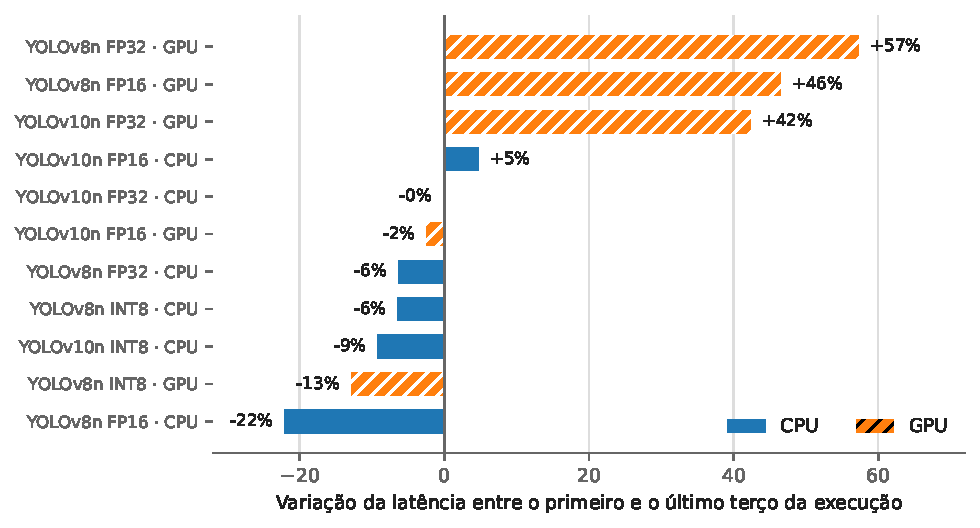
\includegraphics[width=0.82\textwidth,height=0.33\textheight,keepaspectratio]{figuras/deriva_execucao.pdf}}
    \legend{Elaborada pela autora (2026).}
\end{figure}

\FloatBarrier

Três das cinco execuções em \ac{GPU} apresentam degradação progressiva acentuada, com aumento de 42\% a 57\% entre o primeiro e o último terço da sequência. Nenhuma execução em \ac{CPU} apresenta esse comportamento; ao contrário, todas permanecem estáveis ou apresentam leve melhora, atribuível ao término do aquecimento dos \textit{caches}.

O padrão é compatível com limitação térmica da \ac{GPU}, uma vez que a carga sustentada por alguns minutos eleva a temperatura do encapsulamento e o governador de frequência reduz o \textit{clock} do acelerador. Duas execuções em \ac{GPU} não exibiram a degradação, o que indica que o fenômeno depende do estado térmico inicial do dispositivo e não se manifesta invariavelmente. Essa dependência não foi controlada experimentalmente e constitui limitação do protocolo adotado, registrada na Subseção~\ref{sec:limitacoes}.

A consequência prática é que o ganho de 4,7$\times$ do \textit{delegate} \ac{GPU} sobre o YOLOv8n não se sustenta integralmente em uso contínuo. Para captura esporádica, que é o padrão de uso previsto para a aplicação, o ganho é real e imediato. Para processamento em lote prolongado, a vantagem reduz-se à medida que o dispositivo aquece, ainda que permaneça relevante, pois mesmo no último terço a latência em \ac{GPU} (77,9~ms) permanece quase quatro vezes inferior à média em \ac{CPU}.

\subsubsection{Decomposição da latência total}
\label{sec:decomposicao_latencia}

A latência total por imagem, que inclui o pré-processamento, a inferência e o pós-processamento, situou-se entre 1.621 e 2.294~ms em todas as configurações. A inferência responde por parcela minoritária desse total, conforme apresentado na Figura~\ref{fig:composicao_latencia}.

\begin{figure}[H]
    \centering
    \caption{Composição da latência total por etapa de processamento}
    \label{fig:composicao_latencia}
    \figuraMedia{figuras/composicao_latencia.pdf}
    \legend{Elaborada pela autora (2026).}
\end{figure}

\FloatBarrier

O pré-processamento, que compreende a decodificação do arquivo JPEG, o redimensionamento com preservação de proporção e preenchimento do \textit{buffer} de entrada, conforme descrito na Subseção~\ref{sec:aplicacao_android}, consumiu entre 1.429 e 1.885~ms, correspondendo a 77\% a 96\% da latência total conforme a configuração. O pós-processamento, incluindo a \ac{NMS} no YOLOv8n, manteve-se abaixo de 1~ms em todas as execuções, tornando-se desprezível.

Esse resultado qualifica a leitura dos demais. A redução de 303,6 para 64,5~ms na inferência do YOLOv8n, ganho de 4,71$\times$, traduz-se em redução de 1.963 para 1.621~ms na latência total, ganho de apenas 1,21$\times$. Do ponto de vista do usuário, portanto, a escolha do \textit{delegate} altera a experiência de uso em grau inferior ao que a comparação de inferência isolada sugere.

Em consequência, a taxa de processamento, calculada conforme a Equação~\ref{eq:fps} a partir da latência total, permaneceu abaixo de um quadro por segundo em todas as configurações, variando entre 0,44 e 0,62 quadros por segundo. A aplicação, na forma implementada, não opera em tempo real.

A implicação metodológica é que, nas condições medidas, o gargalo da aplicação não está no modelo nem no acelerador, mas na preparação da imagem em código Dart. Otimizações nessa etapa, como a decodificação nativa e o redimensionamento por biblioteca de plataforma, produziriam ganho superior ao obtido pela substituição do \textit{delegate}. Essa constatação não invalida a comparação entre \textit{delegates}, que é o objeto deste trabalho, mas delimita seu alcance.

\subsubsection{Memória e consumo energético}
\label{sec:memoria_energia}

O pico de memória observado variou entre 536 e 750~MB sem relação monotônica com a precisão do modelo ou com o \textit{delegate}. O menor pico foi registrado em YOLOv8n \ac{FP16} com \ac{GPU} (536~MB) e o maior em YOLOv8n \ac{INT8} com \ac{GPU} (750~MB), configurações cujos arquivos de modelo diferem em menos de 3~MB. A medição reflete o uso de memória do processo inteiro, incluindo o \textit{heap} do Dart e os \textit{buffers} de imagem decodificada, e não isola o interpretador do \ac{TFLite}; não permite, portanto, atribuir o consumo ao modelo.

O consumo energético foi de 4\% da carga da bateria nas execuções do YOLOv8n e de 4\% a 5\% nas do YOLOv10n, em sessões de 472 a 661 segundos. A resolução de 1\% do sensor de bateria é insuficiente para discriminar entre configurações, e as leituras não sustentam comparação. Uma medição energética adequada exigiria instrumentação externa, fora do escopo deste trabalho.

\subsubsection{Síntese}
\label{sec:sintese_movel}

Os resultados sustentam quatro conclusões.

A primeira é que o \textit{delegate} \ac{GPU} acelera o YOLOv8n, reduzindo a latência de inferência por fator de 3,6 a 4,7 conforme a precisão.

A segunda é que esse ganho não se estende ao YOLOv10n. As operações que implementam sua arquitetura sem \ac{NMS} não são suportadas pelo \textit{delegate} \ac{GPU}, o que leva à partição do grafo e, na precisão \ac{INT8}, à falha de execução. Em um dispositivo cuja aceleração disponível seja a \ac{GPU}, o YOLOv10n não oferece vantagem sobre o YOLOv8n, e sim desvantagem.

A terceira é que a quantização \ac{FP16} preserva a saída dos modelos pela metade do espaço em disco, enquanto a quantização \ac{INT8} introduz variação no número de detecções, com indício de falsos positivos.

A quarta é que, neste aparelho, as configurações mais rápidas são as menos estáveis, e as execuções em \ac{GPU} apresentaram degradação progressiva ao longo da sessão, com perda de até 57\% de desempenho em poucos minutos. A coleta relatada na Subseção~\ref{sec:dispersao_multidispositivo} mostra que a maior dispersão em \ac{GPU} não se reproduz nos demais aparelhos sobre execuções mais curtas, de modo que essa conclusão permanece circunscrita à plataforma avaliada.

Para a aplicação proposta, a configuração recomendada é \textbf{YOLOv8n \ac{FP16} com \textit{delegate} \ac{GPU}}, que apresentou latência de inferência de 69,2~ms, arquivo de 6,02~MB, saída equivalente à do modelo em precisão plena e o menor pico de memória entre todas as configurações medidas.

\FloatBarrier

\subsection{Desempenho em Múltiplos Dispositivos}
\label{sec:multidispositivo}

A Tabela~\ref{tab:aparelhos} apresenta os sete aparelhos em que foi conduzida
a coleta descrita na Subseção~\ref{sec:coleta_multidispositivo}. O conjunto
abrange os três fornecedores de \ac{SoC} presentes no mercado Android, cobre
da faixa de entrada ao segmento superior e reúne cinco versões do sistema
operacional, do Android~12 ao Android~17. Dois pares de aparelhos compartilham
o mesmo identificador de \textit{hardware} ou o mesmo fornecedor com modelos
distintos, o que permite distinguir o que decorre do fornecedor do que decorre
do aparelho.

\begin{table}[H]
\centering
\caption{Aparelhos empregados na avaliação multidispositivo}
\label{tab:aparelhos}
\begin{tabular}{llccc}
\toprule
\textbf{Aparelho} & \textbf{\ac{SoC}} & \textbf{Android} &
\textbf{Configurações} & \textbf{Sessões} \\
\midrule
Galaxy S24 & Exynos 2400 & 17 & 11 & 3 \\
Redmi Note 9 & MediaTek Helio G85 & 12 & 11 & 1 \\
\bottomrule
\end{tabular}
\legend{Elaborada pela autora (2026).}
\end{table}


A latência média de inferência de cada configuração em cada aparelho consta da
Tabela~\ref{tab:inferencia_dispositivos}. Na mesma configuração, a distância
entre o aparelho mais rápido e o mais lento alcança uma ordem de grandeza, o
que corresponde à diferença entre as plataformas avaliadas.

\begin{table}[H]
\centering
\caption{Latência média de inferência, em milissegundos, por
configuração e aparelho}
\label{tab:inferencia_dispositivos}
\begin{tabular}{llrr}
\toprule
\textbf{Modelo} & \textbf{\textit{Delegate}} & \textbf{S24} & \textbf{Redmi 9} \\
\midrule
YOLOv8n FP32 & \ac{CPU} & 285,4 & 1.076,1 \\
YOLOv8n FP32 & \ac{GPU} & 56,0 & 514,5 \\
YOLOv8n FP16 & \ac{CPU} & 387,5 & 1.119,9 \\
YOLOv8n FP16 & \ac{GPU} & 81,2 & 516,3 \\
YOLOv8n INT8 & \ac{CPU} & 394,4 & 682,7 \\
YOLOv8n INT8 & \ac{GPU} & 109,5 & 559,0 \\
\midrule
YOLOv10n FP32 & \ac{CPU} & 393,3 & 1.652,0 \\
YOLOv10n FP32 & \ac{GPU} & 538,7 & 2.760,7 \\
YOLOv10n FP16 & \ac{CPU} & 404,0 & 1.562,1 \\
YOLOv10n FP16 & \ac{GPU} & 536,8 & 2.701,6 \\
YOLOv10n INT8 & \ac{CPU} & 554,2 & 1.330,5 \\
YOLOv10n INT8 & \ac{GPU} & -- & -- \\
\bottomrule
\end{tabular}
\legend{Elaborada pela autora (2026).}
\end{table}


O resultado de maior interesse não está nos valores absolutos, e sim na razão
entre a execução em \ac{CPU} e em \ac{GPU}, apresentada na
Tabela~\ref{tab:ganho_gpu_dispositivos}. O sentido do efeito do
\textit{delegate} \ac{GPU} é o mesmo nos sete aparelhos. O YOLOv8n é acelerado
em todas as plataformas, por fator entre 1,48 e 7,28, ao passo que no YOLOv10n
o \textit{delegate} não produz ganho em nenhuma delas, com razões entre 0,58 e
0,97. A combinação YOLOv10n/\ac{INT8}/\ac{GPU} não executou em aparelho algum. A Figura~\ref{fig:razao_delegates} dispõe essas razões em escala logarítmica, em que reduzir à metade e dobrar guardam a mesma distância da unidade, e torna visível a separação entre as duas arquiteturas.

\begin{figure}[H]
    \centering
    \caption{Razão entre a inferência em processador e em processador gráfico, por aparelho, arquitetura e precisão}
    \label{fig:razao_delegates}
    \figuraHorizontal{figuras/razao_delegates.pdf}
    \legend{Elaborada pela autora (2026). Os aparelhos aparecem ordenados pela latência de inferência do YOLOv8n \ac{FP32} em \ac{CPU}, do mais lento ao mais rápido. A faixa sombreada reúne as razões inferiores à unidade.}
\end{figure}

\begin{table}[H]
\centering
\caption{Razão entre a inferência em processador e em processador
gráfico, por aparelho}
\label{tab:ganho_gpu_dispositivos}
\begin{tabular}{lcc}
\toprule
\textbf{Configuração} & \textbf{S24} & \textbf{Redmi 9} \\
\midrule
YOLOv8n FP32 & 5,10$\times$ & 2,09$\times$ \\
YOLOv8n FP16 & 4,77$\times$ & 2,17$\times$ \\
YOLOv8n INT8 & 3,60$\times$ & 1,22$\times$ \\
\midrule
YOLOv10n FP32 & 0,73$\times$ & 0,60$\times$ \\
YOLOv10n FP16 & 0,75$\times$ & 0,58$\times$ \\
YOLOv10n INT8 & -- & -- \\
\bottomrule
\end{tabular}
\legend{Elaborada pela autora (2026). Valores acima da unidade indicam
ganho do \textit{delegate} de processador gráfico. O traço assinala
configuração que não executou.}
\end{table}


A única exceção ao ganho do YOLOv8n ocorre no moto~g15 na precisão \ac{INT8},
com razão de 0,87. A magnitude do ganho varia por fator superior a quatro
entre o maior e o menor valor observado e acompanha a faixa de desempenho do
aparelho, de modo que o ganho do \textit{delegate} \ac{GPU} constitui
resultado de plataforma, e não propriedade fixa do modelo. A direção do
efeito, por outro lado, não depende do fornecedor nem da versão do sistema, o
que sustenta a interpretação apresentada na Subseção~\ref{sec:v10n_gpu},
segundo a qual a incompatibilidade do YOLOv10n decorre da cobertura de
operações do \textit{delegate} e não de característica do aparelho de
referência.

\subsubsection{Estabilidade das detecções entre aparelhos}
\label{sec:estabilidade_deteccoes}

A comparação das saídas verifica se o mesmo modelo produz as mesmas detecções
em plataformas distintas. Em dez das onze configurações executáveis, o número
de detecções coincide em todos os aparelhos, imagem por imagem, perfazendo 310
concordâncias em 321 comparações.

A exceção é o YOLOv8n em \ac{INT8} com \textit{delegate} \ac{GPU}, em que 11
das 26 imagens comuns aos sete aparelhos apresentam contagens distintas, com
diferença de uma ou duas detecções. Trata-se da única configuração que reúne
quantização inteira e execução em \ac{GPU}, e a divergência é compatível com a
variação da implementação dos núcleos quantizados entre fornecedores, uma vez
que a mesma quantização executada em \ac{CPU} produz contagens idênticas nos
sete aparelhos.

Registre-se que o total acumulado nessas 26 imagens é de 275 detecções em
todos os sete aparelhos, pois as diferenças individuais se compensam. A
leitura por totais indicaria concordância completa, e apenas a comparação
imagem a imagem revela a divergência, o que recomenda cautela no uso de
indicadores agregados para verificar equivalência de saída.

\subsubsection{Dispersão dentro da execução}
\label{sec:dispersao_multidispositivo}

A Subseção~\ref{sec:estabilidade} registrou, no aparelho de referência,
coeficiente de variação superior nas execuções em \ac{GPU}. A
Figura~\ref{fig:dispersao_execucao} apresenta esse coeficiente em cada
configuração, com um ponto por aparelho, e mostra que a associação não se
repete fora daquela plataforma.

\begin{figure}[H]
    \centering
    \caption{Coeficiente de variação da latência de inferência dentro de cada
    execução, por configuração, com um ponto por aparelho}
    \label{fig:dispersao_execucao}
    \figuraHorizontal{figuras/dispersao_execucao.pdf}
    \legend{Elaborada pela autora (2026).}
\end{figure}

Considerada a mediana das configurações de cada aparelho, a dispersão em
\ac{GPU} supera a observada em \ac{CPU} apenas no aparelho de referência,
com 9,9\% contra 7,8\%. Nos seis demais a relação se inverte, com valores
entre 0,9\% e 4,2\% em \ac{GPU} contra 1,7\% e 8,9\% em \ac{CPU}. A
maior dispersão em \ac{GPU} não constitui, portanto, propriedade do
\textit{delegate}.

Essa comparação não refuta a deriva relatada na
Subseção~\ref{sec:estabilidade}, e sim delimita o que dela se pode
generalizar. As execuções desta coleta percorrem 30 imagens, contra as 285 da
avaliação no aparelho de referência, e a deriva ali documentada se acumula ao
longo da execução, de modo que uma execução dez vezes mais curta oferece menos
oportunidade para que ela se manifeste. Verificar se a deriva ocorre nos demais
aparelhos exigiria execuções de duração comparável, o que não foi solicitado
aos voluntários.

\subsubsection{Variação entre execuções de uma mesma configuração}
\label{sec:repetibilidade}

A variação da latência de inferência entre as três sessões realizadas no
aparelho de referência consta da Tabela~\ref{tab:sessoes}. A amplitude entre a
maior e a menor média obtidas para a mesma configuração corresponde a 18,6\%
da média na mediana das onze configurações e alcança 32,1\% no YOLOv8n em
\ac{INT8} com \textit{delegate} \ac{GPU}.

\begin{table}[H]
\centering
\small
\caption{Variação da latência de inferência entre sessões repetidas do
mesmo aparelho, em milissegundos}
\label{tab:sessoes}
\begin{tabular}{llrrr}
\toprule
\textbf{Modelo} & \textbf{\textit{Delegate}} & \multicolumn{3}{c}{\textbf{S24}} \\
 & & \textbf{Média} & \textbf{Amplitude} & \textbf{\%} \\
\midrule
YOLOv8n FP32 & \ac{CPU} & 294,1 & 44,9 & 15,3 \\
YOLOv8n FP32 & \ac{GPU} & 55,6 & 4,1 & 7,3 \\
YOLOv8n FP16 & \ac{CPU} & 361,1 & 137,2 & 38,0 \\
YOLOv8n FP16 & \ac{GPU} & 84,3 & 22,7 & 26,9 \\
YOLOv8n INT8 & \ac{CPU} & 392,1 & 14,5 & 3,7 \\
YOLOv8n INT8 & \ac{GPU} & 109,9 & 35,1 & 32,0 \\
\midrule
YOLOv10n FP32 & \ac{CPU} & 390,8 & 95,3 & 24,4 \\
YOLOv10n FP32 & \ac{GPU} & 524,7 & 92,8 & 17,7 \\
YOLOv10n FP16 & \ac{CPU} & 403,8 & 75,1 & 18,6 \\
YOLOv10n FP16 & \ac{GPU} & 541,1 & 132,7 & 24,5 \\
YOLOv10n INT8 & \ac{CPU} & 550,0 & 95,2 & 17,3 \\
\bottomrule
\end{tabular}
\legend{Elaborada pela autora (2026). Em S24, 4 sessões sobre Android 17. A amplitude é a diferença
entre a maior e a menor média obtidas para a mesma configuração em
sessões distintas, e a última coluna exprime essa amplitude como
percentual da média.}
\end{table}


As configurações executadas em \ac{CPU} apresentam amplitude entre 2,3\% e
24,2\%, ao passo que as executadas em \ac{GPU} situam-se entre 7,3\% e 32,1\%,
o que é coerente com a menor estabilidade do \textit{delegate} \ac{GPU}
registrada na Subseção~\ref{sec:estabilidade}.

Essa medida define a resolução do experimento. Diferenças de latência
inferiores a cerca de 20\% entre duas configurações não se distinguem da
variação observada em repetições de uma mesma configuração, de modo que as
comparações deste capítulo que recaem nessa faixa devem ser lidas como
equivalência, e não como ordenação. As razões entre \ac{CPU} e \ac{GPU}
discutidas nesta subseção situam-se fora dessa faixa no YOLOv8n, em que a
menor delas corresponde a redução de 32\% da latência. No YOLOv10n as razões
próximas da unidade indicam ausência de ganho, afirmação que não depende de
ordenar configurações dentro da faixa de equivalência.

\subsubsection{Desvios de protocolo e seus efeitos}
\label{sec:desvios_protocolo}

Dois desvios em relação ao protocolo foram identificados nos arquivos
recebidos. O efeito de cada um foi medido antes da decisão de manter os dados
correspondentes.

No Galaxy A15 5G e no Galaxy S23 as execuções foram precedidas de três
inferências de aquecimento, e não de dez. Caso o aquecimento fosse
insuficiente, as primeiras medições de cada execução seriam superiores às
demais. A média das três primeiras medições fica 1,0\% abaixo da média das
restantes nesses dois aparelhos, contra 0,6\% abaixo nos cinco que executaram
dez inferências de aquecimento, valor situado dentro da faixa observada entre
os próprios aparelhos que cumpriram o protocolo. O aquecimento reduzido não
deslocou as médias.

No moto~g15 a coleta iniciou com 54\% de carga, abaixo dos 80\% previstos, e a
carga decresceu até 47\% ao longo da varredura. As três configurações do
YOLOv10n em \ac{CPU}, medidas a 51\%, 49\% e 48\% de carga, apresentaram
1.058,76, 1.061,50 e 1.060,32~ms de inferência, com dispersão de 0,26\% entre
elas. Redução de frequência por nível de carga produziria valores crescentes
ao longo da sessão, comportamento que não se observa.

Ambos os desvios permanecem registrados na Subseção~\ref{sec:limitacoes}, uma
vez que a ausência de efeito mensurável nas medições disponíveis não equivale
a garantia de ausência de efeito.

\FloatBarrier

\subsection{Limitações}
\label{sec:limitacoes}

Os resultados apresentados estão condicionados por um conjunto de limitações de escopo e de protocolo, descritas a seguir.

\subsubsection{Limitações do protocolo experimental}

\textbf{Aparelho único na avaliação sobre o conjunto completo.} A avaliação sobre as 285 imagens da partição de teste foi conduzida em um único aparelho, pelas razões expostas na Subseção~\ref{sec:dispositivo}. A coleta descrita na Subseção~\ref{sec:coleta_multidispositivo} estendeu a avaliação a sete aparelhos, porém sobre o subconjunto de 30 imagens, de modo que os valores absolutos de latência reportados nas tabelas da Subseção~\ref{sec:resultados_movel} permanecem condicionados a uma plataforma. O que a coleta posterior sustenta é o sentido do efeito do \textit{delegate}, verificado nos sete aparelhos, e não a magnitude registrada naquelas tabelas, que varia por fator superior a quatro entre as plataformas avaliadas.

\textbf{Execução única sobre o conjunto completo.} Cada configuração foi executada uma única vez sobre as 285 imagens da partição de teste. A repetição conduzida sobre o subconjunto de 30 imagens, relatada na Subseção~\ref{sec:repetibilidade}, fornece a ordem de grandeza da variação entre execuções de uma mesma configuração, que é de 18,6\% na mediana das onze configurações e alcança 32,1\%. Esse valor foi obtido no aparelho de referência e sobre o subconjunto, e seu transporte para as medições sobre o conjunto completo e para os demais aparelhos constitui suposição, não verificação. Diferenças entre configurações próximas permanecem, portanto, sujeitas a reserva.

\textbf{Estado térmico não controlado.} As execuções foram distribuídas em dois dias e em horários distintos, sem padronização do intervalo de repouso entre elas nem verificação da temperatura inicial do aparelho. A análise de deriva apresentada na Subseção~\ref{sec:estabilidade} indica que o estado térmico afeta o desempenho em \ac{GPU} de forma desigual, uma vez que três execuções apresentaram degradação superior a 40\% e duas não apresentaram degradação alguma. Essa variação não foi controlada e constitui a limitação mais relevante do protocolo quanto às medidas de estabilidade.

\textbf{Nível de carga não padronizado na avaliação principal.} Na avaliação sobre o conjunto completo o nível de bateria no início das execuções variou entre 49\% e 94\%. Sistemas Android podem reduzir a frequência de operação em níveis baixos de carga, ainda que o modo de economia de energia esteja desativado. A influência desse fator sobre essas medições não foi isolada. A coleta em múltiplos dispositivos adotou limiar fixo de 80\%, cumprido em seis dos sete aparelhos.

\textbf{Desvios de protocolo na coleta em múltiplos dispositivos.} Dois aparelhos executaram com três inferências de aquecimento, e não com dez, e um iniciou a coleta com 54\% de carga. Os efeitos foram medidos e estão relatados na Subseção~\ref{sec:desvios_protocolo}, sem que se tenha observado deslocamento das médias em nenhum dos dois casos. A ausência de efeito mensurável nas medições disponíveis não equivale, contudo, a garantia de ausência de efeito, e os aparelhos foram mantidos no conjunto analisado com essa ressalva.

\subsubsection{Limitações das medidas}

\textbf{Memória.} A medida de memória corresponde ao conjunto residente do processo da aplicação, incluindo o \textit{heap} do ambiente de execução Dart e os \textit{buffers} de imagem decodificada. Não isola o consumo do interpretador do \ac{TFLite} e, portanto, não permite atribuir o pico observado ao modelo.

\textbf{Consumo energético.} A resolução de 1\% da interface de bateria do Android é insuficiente para discriminar entre configurações em sessões da duração empregada. Os valores reportados indicam apenas a ordem de grandeza do consumo e não sustentam comparação. Uma avaliação energética adequada exigiria instrumentação externa.

\textbf{Temperatura.} Não foi possível incorporar a temperatura do dispositivo ao conjunto de métricas coletadas automaticamente, conforme registrado na Subseção~\ref{sec:aplicacao_android}. A degradação térmica foi, portanto, inferida indiretamente a partir da deriva da latência, e não medida. Protocolos de avaliação de inferência em dispositivos móveis recorrem à fixação das frequências de operação e ao resfriamento ativo do aparelho para conter esse efeito \cite{Li2024Benchmark}, recursos incompatíveis com uma coleta conduzida por terceiros em aparelhos próprios.

\subsubsection{Limitações do conjunto de dados}

\textbf{Casos residuais de anotação agrupada.} A reanotação semi-automática descrita na Subseção~\ref{sec:preprocessamento} eliminou as delimitações correspondentes a agrupamentos extensos, mas permanecem casos em que frutos adjacentes ou parcialmente sobrepostos continuam delimitados por uma única caixa. Esses casos penalizam a correspondência entre predições e anotações independentemente da detecção efetiva dos frutos, e contribuem para os valores de revocação observados.

\textbf{Conjunto parcialmente anotado.} Das aproximadamente 5.000 imagens adquiridas em campo, 2.168 compõem o conjunto utilizado. A ampliação do conjunto anotado constitui possibilidade de continuidade.

\textbf{Efeito da quantização \ac{INT8} sobre as detecções.} O aumento no número de detecções observado nas variantes \ac{INT8}, descrito na Subseção~\ref{sec:efeito_quantizacao}, é compatível com a introdução de falsos positivos, mas essa interpretação não foi verificada, uma vez que a confrontação das detecções produzidas no dispositivo com as anotações de referência não foi conduzida.

\subsubsection{Limitações de escopo}

\textbf{Pré-processamento não otimizado.} Conforme demonstrado na Subseção~\ref{sec:decomposicao_latencia}, a preparação da imagem responde pela maior parte da latência total. A implementação adotada reproduz o procedimento utilizado no treinamento e não foi objeto de otimização, uma vez que o objeto do trabalho é a comparação entre \textit{delegates}. Os valores de latência total aqui reportados não devem ser lidos como limite da plataforma.

\textbf{\textit{Delegate} NNAPI não avaliado.} A \ac{NNAPI}, que direciona a inferência a aceleradores dedicados do \ac{SoC}, foi depreciada a partir do Android~15, e a própria documentação recomenda a migração para o \ac{TFLite} \cite{Android2026NNAPI}. Como o dispositivo utilizado executa Android~16, a avaliação restringiu-se aos \textit{delegates} de \ac{CPU} e \ac{GPU}. O acesso a unidades de processamento neural em versões recentes do Android depende de bibliotecas específicas de cada fornecedor, cuja avaliação extrapola o escopo deste trabalho.

\textbf{Classificação do estágio de maturação.} A detecção dos frutos foi conduzida com classe única, transferindo a determinação do estágio de maturação para etapa subsequente. A implementação e a avaliação dessa etapa não integram os resultados aqui reportados.

\FloatBarrier

\section{CONCLUSÃO}
\label{sec:conclusao}

Este trabalho comparou configurações dos modelos YOLOv8n e YOLOv10n convertidos para \ac{TFLite} quanto ao desempenho e à estabilidade de execução em \textit{smartphone} Android, no contexto da detecção de frutos de café em lavouras de campo aberto.

Foram conduzidas a construção e a curadoria de um conjunto de 2.168 imagens próprias com 17.659 instâncias anotadas, o treinamento das duas arquiteturas, a conversão para \ac{TFLite} em três precisões numéricas, o desenvolvimento de uma aplicação Android para execução local dos modelos e a medição de onze das doze configurações experimentais previstas.

\subsection{Quanto aos Objetivos}

Os modelos treinados apresentaram desempenho de detecção equivalente, com \ac{mAP}@0,50 de 0,6455 para o YOLOv8n e 0,6419 para o YOLOv10n sobre o conjunto de teste. A conversão preservou esse desempenho, com diferenças inferiores a 0,002 nas variantes em precisão plena.

A comparação entre \textit{delegates}, objetivo central do trabalho, produziu o resultado mais relevante. O \textit{delegate} \ac{GPU} reduziu a latência de inferência do YOLOv8n por fator entre 3,58 e 4,72, conforme a precisão. No YOLOv10n o mesmo \textit{delegate} não produziu ganho, pois em \ac{FP32} a latência aumentou em 47\%, em \ac{FP16} permaneceu equivalente à obtida em \ac{CPU} e na precisão \ac{INT8} a execução não é possível.

A causa está na própria arquitetura. A supressão da etapa de \ac{NMS}, que constitui a contribuição central do YOLOv10, é obtida por meio de operações como \texttt{TOPK\_V2}, \texttt{GATHER\_ND} e conversões para \texttt{INT64}, que o \textit{delegate} \ac{GPU} do \ac{TFLite} não suporta. O grafo é então particionado entre os dois processadores, e o custo das transferências entre suas memórias anula o ganho obtido nos segmentos delegados. Na precisão \ac{INT8} a fragmentação é acentuada, com apenas 13 das 345 operações delegadas, e a execução termina em erro.

Quanto à quantização, as duas estratégias apresentaram comportamento distinto. A precisão \ac{FP16} preservou a saída dos modelos, pois no YOLOv8n em \ac{CPU} as variantes \ac{FP32} e \ac{FP16} produziram exatamente o mesmo número de detecções sobre as 285 imagens, pela metade do tamanho de arquivo. A precisão \ac{INT8} alterou a saída, com acréscimo de 5,1\% no número de detecções do YOLOv8n, compatível com a introdução de falsos positivos.

Quanto à estabilidade, observou-se no aparelho de referência relação inversa à da latência, uma vez que as configurações mais rápidas apresentaram maior dispersão relativa. As execuções em \ac{GPU} apresentaram coeficiente de variação entre 19,5\% e 28,5\%, contra 10,6\% a 20,5\% em \ac{CPU}, e três delas degradaram entre 42\% e 57\% ao longo de uma única sessão, comportamento compatível com limitação térmica e ausente em todas as execuções em \ac{CPU}. Essa relação não se reproduziu nos demais aparelhos sobre execuções mais curtas, conforme a Subseção~\ref{sec:dispersao_multidispositivo}, de modo que permanece circunscrita à plataforma em que foi medida.

\subsection{Quanto às Hipóteses Formuladas}

Duas previsões formuladas a partir dos resultados de treinamento não se confirmaram na execução em dispositivo, e seu exame constitui parte do que o trabalho acrescenta.

A primeira supunha que a vantagem do YOLOv10n no tempo de pós-processamento, de aproximadamente 4,1 vezes em ambiente de desenvolvimento, seria proporcionalmente maior em processadores móveis. A previsão não se verificou. O pós-processamento permaneceu abaixo de 1~ms em todas as onze configurações, inclusive naquelas que executam supressão não máxima, de modo que a vantagem existe, mas incide sobre uma parcela desprezível da latência total e não se traduz em benefício perceptível.

A segunda supunha que o menor custo computacional do YOLOv10n, com 24,6\% menos parâmetros e 19,8\% menos operações de ponto flutuante, o tornaria mais adequado à execução embarcada. O resultado foi o oposto. Na presença de \textit{delegate} \ac{GPU}, o YOLOv10n é a escolha mais lenta por margem ampla, e sua variante de menor arquivo não é executável.

A extensão da avaliação a sete aparelhos, descrita na Subseção~\ref{sec:multidispositivo}, verificou o alcance desse resultado. O sentido do efeito do \textit{delegate} \ac{GPU} repete-se em todos eles, com aceleração do YOLOv8n por fator entre 1,48 e 7,28 e ausência de ganho no YOLOv10n, cuja variante \ac{INT8} não executa em aparelho algum. A magnitude, por outro lado, varia por fator superior a quatro entre as plataformas, de modo que o ganho constitui resultado de plataforma e não propriedade do modelo. Em dez das onze configurações executáveis o número de detecções coincide em todos os aparelhos, imagem por imagem.

O exame conjunto dessas duas previsões sugere uma conclusão de alcance mais geral, segundo a qual os indicadores de custo computacional medidos em ambiente de desenvolvimento, como o número de parâmetros, as operações de ponto flutuante e o tempo de pós-processamento, não predizem o desempenho em dispositivo móvel quando há aceleração por \textit{hardware} envolvida. O fator determinante não é o volume de computação exigido pelo modelo,
mas a compatibilidade entre as operações que ele emprega e aquelas que o
acelerador implementa.

Uma terceira observação, de porte menor, aponta no mesmo sentido e antecede
a saída do modelo do ambiente de treinamento. Conforme a
Subseção~\ref{sec:desempenho_deteccao}, a ordem entre as duas arquiteturas
quanto ao tempo de inferência depende do preenchimento aplicado às imagens.
Sob o agrupamento retangular por lote, o YOLOv10n é mais rápido. Sob o
preenchimento quadrado que a aplicação executa no aparelho, é mais lento, e
as faixas das três execuções de cada arquitetura não se sobrepõem. A
comparação entre arquiteturas não constitui, portanto, propriedade das
arquiteturas tomadas isoladamente, e sim do conjunto formado por elas, pelo
preenchimento da entrada e pelo processador que as executa. É a mesma
dependência que a comparação entre \textit{delegates} evidencia, observável
já dentro do ambiente de desenvolvimento.

\subsection{Recomendação}

Para a aplicação proposta, a configuração recomendada é o \textbf{YOLOv8n em precisão \ac{FP16} com \textit{delegate} \ac{GPU}}, que apresentou latência de inferência de 69,2~ms, arquivo de 6,02~MB, saída equivalente à da variante em precisão plena e o menor pico de memória entre as configurações avaliadas.

Para dispositivos sem \textit{delegate} \ac{GPU} funcional, a recomendação passa ao YOLOv8n em \ac{FP32} com \textit{delegate} de \ac{CPU}, que apresentou a menor latência entre as execuções em processador central.

\subsection{Quanto à Classificação do Estágio de Maturação}
\label{sec:quanto_maturacao}

A detecção foi conduzida com classe única, de modo que o trabalho localiza frutos e não determina o estágio de maturação de cada um. Cabe expor a razão dessa delimitação, uma vez que o problema de origem, enunciado na Seção~\ref{sec:introducao}, é a avaliação da maturação.

A primeira razão está no conjunto de dados. A anotação em duas classes considerada durante a construção do conjunto, descrita na Subseção~\ref{sec:anotacao}, distingue cultivares de fruto vermelho e amarelo, e não estágios de maturação de um mesmo fruto. Classificar maturação exigiria reanotar as 17.659 instâncias segundo estágios, tarefa de natureza distinta da que foi executada e de porte comparável ao da construção do conjunto.

A segunda razão está nos resultados de detecção. A revocação obtida é de 0,6132 no YOLOv8n sobre o conjunto de teste, de modo que aproximadamente 39\% dos frutos anotados não são localizados. Classificar o estágio de frutos que o detector não encontra não melhora a estimativa de maturação do talhão, e a precisão da localização constitui, portanto, a restrição que vincula o resultado final. Trabalhos que classificam maturação de frutos de café em campo partem de detectores ajustados a esse fim \cite{Ye2025ASD, Kazama2024Monitoring}, o que reforça a ordem adotada aqui.

A terceira razão é de escopo. O objeto declarado deste trabalho é a comparação entre \textit{delegates} do \ac{TFLite} quanto a desempenho e estabilidade, e essa comparação não depende do número de classes do modelo. A classe única mantém o problema de detecção estável enquanto variam arquitetura, precisão numérica e mecanismo de aceleração, que são os fatores sob exame.

A arquitetura de duas etapas, com detecção seguida de classificação dos recortes, permanece como caminho preparado. A detecção com classe única produz exatamente a entrada de que a etapa seguinte necessita.

\subsection{Trabalhos Futuros}

A continuidade natural da pesquisa é a classificação do estágio de maturação dos frutos detectados, etapa para a qual a detecção com classe única foi deliberadamente preparada.

A avaliação em outros aparelhos, prevista como continuidade, foi conduzida e integra os resultados. Resta estendê-la em duas direções. A primeira é a medição sobre o conjunto de teste completo nos aparelhos de terceiros, uma vez que as execuções sobre 30 imagens não permitem observar a deriva ao longo da sessão, discutida na Subseção~\ref{sec:dispersao_multidispositivo}. A segunda é a inclusão de aparelhos com unidade de processamento neural acessível por biblioteca do fornecedor, caminho que a depreciação da \ac{NNAPI} tornou o único disponível para esse tipo de acelerador.

A medição direta da temperatura do aparelho, ausente nesta coleta, permitiria substituir por verificação a atribuição da deriva a limitação térmica, hoje apenas compatível com os dados. A instrumentação necessária está descrita em protocolos de avaliação de inferência móvel \cite{Li2024Benchmark}.

A otimização do pré-processamento, responsável pela maior parte da latência total, produziria ganho superior ao obtido pela substituição do \textit{delegate} e constitui a intervenção de maior efeito prático sobre a aplicação.

Por fim, a confrontação das detecções produzidas no dispositivo com as anotações de referência permitiria verificar a hipótese de introdução de falsos positivos pela quantização \ac{INT8}, aqui apenas sugerida pelo acréscimo no número de detecções.

\section*{REFERÊNCIAS}

\printbibliography

\attachment

\end{document}
